\documentclass[12pt,letterpaper]{article}
\usepackage{OSUDissertation}

\begin{document}
%%%%%%%%%%%%%%%%%%%%%%%%%%%%%%%%%%%%%%%
\section{Results}
\label{sec:Results}
This section presents all of the results that were performed utilizing the methods described in Section~\ref{sec:Methods}. In Section~\ref{sec:ResultsXY}, we discuss results from the implementation of the \XY\ geometry spatial discretization described in Section~\ref{sec:HODFEM}. In Section~\ref{sec:ResultsRZ}, we show results from the implementation of the \RZ\ geometry angular and spatial discretizations discussed in Section~\ref{sec:MethodsRZ}. In Section~\ref{sec:ResultsMIP}, we show results from the implementation of the modified interior penalty (MIP) diffusion synthetic acceleration (DSA) discussed in Section~\ref{sec:MIPDSA}.

%%%%%%%%%%%%%%%%%%%%%%%%%%%%%%%%%%%%%%%
\subsection{\XY\ Geometry}
\label{sec:ResultsXY}
In this section, we present additional results in \XY\ geometry to supplement the work done in Woods~\cite{WoodsThesis}. The spatial discretization in this section is discussed in Section~\ref{sec:HODFEM}. We solve a uniform infinite medium problem in Section~\ref{sec:XYuim}. We perform a spatial convergence study in Section~\ref{sec:XYSpatialConv}. In Section~\ref{sec:XYAltInc}, we exercise the methodology on an optically thick and diffusive problem. Finally, we show results that investigate the integration scheme for the surface integrals in Section~\ref{sec:InOutSensitivity}.

%%%%%%%%%%%%%%%%%%%%%%%%%%%%%%%%%%%%%%%
\subsubsection{Uniform Infinite Medium}
\label{sec:XYuim}
We solved a uniform infinite medium problem on a high-order mesh that has sufficient curvature to have incident and outgoing angular fluxes on some mesh surfaces for the same angular direction $\vec{\Omega}$. This solution was obtained using $4^\text{th}$-order finite elements and $S_{12}$ level-symmetric angular quadrature. The homogeneous material has $\sigma_t=1$, $\sigma_a=0.7$, $S_0=0.7$, and has analytic solution $\phi=1$. The mesh is overlaid on top of the solution in Figure~\ref{fig:uim3PointQ4Q3R1p4S12}.
%
\begin{figure}[!htb]
\centering
\includegraphics[scale=0.45,trim={20pt 500pt 20pt 60pt},clip]{../../Research/graphics/uim3PointQ4Q3R1p4S12}
\caption{Uniform infinite medium scalar flux solution.}
\label{fig:uim3PointQ4Q3R1p4S12}
\end{figure}
%
Despite performing numerical integrations of a discontinuous function along some of the surfaces, we still obtain the exact solution for this problem.

%%%%%%%%%%%%%%%%%%%%%%%%%%%%%%%%%%%%%%%
\subsubsection{Spatial convergence on a highly curved mesh}
\label{sec:XYSpatialConv}
We use the manufactured solution
\begin{flalign}
\psi_\text{MMS}(x,y,\mu,\eta) & = (1-\mu^2)(1-\eta^2) \sin(\alpha \pi x) \cos(\beta \pi y)
\label{eq:GleicherMMS}
\end{flalign}

\noindent on a \emph{highly} curved mesh with $\alpha=1$ and $\beta=1/2$. We obtain the analytical source $S_0$ that gives the exact manufactured solution by inserting Equation~\ref{eq:GleicherMMS} into the \XY\ transport equation:
\begin{multline}
\vec{\Omega} \vd \grad \left[(1-\mu^2)(1-\eta^2) \sin(\alpha \pi x) \cos(\beta \pi y) \right] \\
+ \sigma_t \left[(1-\mu^2)(1-\eta^2) \sin(\alpha \pi x) \cos(\beta \pi y) \right] \\
= \frac{1}{4 \pi} \sigma_s\ \phi_\text{MMS} + \frac{1}{4 \pi} S_0,
\end{multline}
%
where
\begin{flalign}
\phi_\text{MMS} & = \int_{4 \pi} \psi_\text{MMS}\ d \Omega, \\
& = \frac{8 \pi}{5} \sin(\alpha \pi x) \cos(\beta \pi y).
\end{flalign}
%
Given,
\begin{multline}
\vec{\Omega} \vd \grad \left[(1-\mu^2)(1-\eta^2) \sin(\alpha \pi x) \cos(\beta \pi y) \right] \\
= \left(1-\mu^2 \right) \left(1-\eta^2 \right) \left[\mu\ \alpha\ \pi \cos(\alpha \pi x) \cos(\beta \pi y) - \eta\ \beta\ \pi \sin(\alpha \pi x) \sin(\beta \pi y) \right]
\end{multline}
%
we obtain the analytical source for the manufactured solution
\begin{multline}
S_0 = 4 \pi \left[\left(1-\mu^2 \right) \left(1-\eta^2 \right) \left(\mu\ \alpha\ \pi \cos(\alpha \pi x) \cos(\beta \pi y) \right. \right. \\
\left. \left. - \eta\ \beta\ \pi \sin(\alpha \pi x) \sin(\beta \pi y) + \sigma_t \sin(\alpha \pi x) \cos(\beta \pi y)  \right) \right. \\
\left. - \frac{8 \pi}{5} \sigma_s\ \sin(\alpha \pi x) \cos(\beta \pi y) \right].
\end{multline}

Reproduced from Woods et al.~\cite{Woods2018HOSnXY}, the solution using $p=4$ and $S_{12}$ level-symmetric angular quadrature is shown in Figure~\ref{fig:Gleicherp4S123Pointv2Q3Q21R} with the coarsest mesh overlaid.
%
\begin{figure}[!htb]
\centering
\includegraphics[scale=0.45,trim={20pt 500pt 20pt 70pt},clip]{../../Research/graphics/Gleicherp4S123Pointv2Q3Q21R}
\caption{MMS solution on a \emph{highly} curved mesh.}
\label{fig:Gleicherp4S123Pointv2Q3Q21R}
\end{figure}
%
Figure~\ref{fig:GleicherS123PointQ3Q2R1Z2p2g-1} shows the errors from a spatial convergence study with select reference lines.
%
\begin{figure}[!htb]
\centering
\begin{tikzpicture}
  \begin{axis}[
    width=0.85\textwidth,
    %height=4.6cm,
    grid=major,
    xlabel={$\sqrt{\text{N}_\text{zones}}$},
    ylabel={L$^2$-error},
  	xmode=log,
  	ymode=log,
  	xmin=3,xmax=1e2,
  	ymin=1e-5,ymax=3,
  	%legend style={at={(1.2,1.1)},anchor=north east},
  	]
\addplot[mark=*, dashed, mark size=2, draw=black, mark options={solid, fill=black}] table [x=un, y=fe1]{../../Research/graphics/GleicherS123PointQ3Q2R1Z2p2g-1.dat};
\addlegendentry{$p=1$}
\addplot[mark=triangle*, dashed, mark size=3, draw=red, mark options={solid, fill=red}] table [x=un, y=fe2]{../../Research/graphics/GleicherS123PointQ3Q2R1Z2p2g-1.dat};
\addlegendentry{$p=2$}
\addplot[mark=square*, dashed, mark size=2, draw=blue, mark options={solid, fill=blue}] table [x=un, y=fe3]{../../Research/graphics/GleicherS123PointQ3Q2R1Z2p2g-1.dat};
\addlegendentry{$p=3$}
\addplot[mark=diamond*, dashed, mark size=3, draw=magenta, mark options={solid, fill=magenta}] table [x=un, y=fe4]{../../Research/graphics/GleicherS123PointQ3Q2R1Z2p2g-1.dat};
\addlegendentry{$p=4$}

\addplot[black] table[row sep=crcr] {
4 1.3 \\
12 .2502 \\};
\node[text=black, anchor=south] at (axis cs:13,0.3) {$O(\frac{3}{2})$};
\addplot[black] table[row sep=crcr] {
25 .04 \\
64 0.0061 \\};
\node[text=black, anchor=west] at (axis cs:40,0.02) {$O(2)$};
\addplot[black] table[row sep=crcr] {
4 0.5 \\
12 .0321 \\};
\node[text=black, anchor=west] at (axis cs:12,0.03) {$O(\frac{5}{2})$};
\addplot[black] table[row sep=crcr] {
12 .02 \\
32 0.0011 \\};
\node[text=black, anchor=west] at (axis cs:8,0.0148){$O(\frac{7}{2})$};
\addplot[black] table[row sep=crcr] {
4 0.1697 \\
8 0.015 \\};
\node[text=black, anchor=west] at (axis cs:25,0.003){$O(3)$};
\addplot[black] table[row sep=crcr] {
8 0.01 \\
16 6.25e-4 \\};
\node[text=black, anchor=west] at (axis cs:13,0.002){$O(4)$};
\addplot[black] table[row sep=crcr] {
4 0.0113 \\
8 5e-4 \\};
\node[text=black, anchor=north east] at (axis cs:5,5e-3){$O(\frac{9}{2})$};
\addplot[black] table[row sep=crcr] {
8 6.4e-4 \\
16 2e-05 \\};
\node[text=black, anchor=east] at (axis cs:15,2e-5){$O(5)$};

  \end{axis}
  
\end{tikzpicture}
\caption{Errors between the manufactured and DFEM solutions. Reference lines depict order of spatial convergence $O(n) \equiv O\left(\left(N_\text{zones} \right)^{n/2} \right)$.}
\label{fig:GleicherS123PointQ3Q2R1Z2p2g-1}
\end{figure}
%
For coarser meshes, we observe degraded convergence rates as low as $O(p+1/2)$. As the mesh is refined, the convergence rates reach $O(p+1)$. This is possibly the effect of the finite element and mesh zone not resolving the solution enough to be in the asymptotic region. Figure~\ref{fig:GleicherS123PointQ3Q2R1Z2p2g-1} reveals that the spatial convergence rates appear to be consistently dependent upon the finite element order.

In this work, we numerically compute all integrals with Gaussian quadrature, which does not accurately integrate functions with discontinuous derivatives. In practice, this mesh would likely be refined and the coarse mesh effects that we observe would be inconsequential.

%%%%%%%%%%%%%%%%%%%%%%%%%%%%%%%%%%%%%%%
\subsubsection{Alternating Incident angular flux Boundary Conditions}
\label{sec:XYAltInc}
This numerical test problem highlights some deficiencies in the DFEM method in the optically thick diffusion limit. The material is homogeneous with no volumetric source, $\sigma_t = 250$, and $\sigma_s = 0.999 \sigma_t$. There are vacuum boundary conditions on all sides except zones with incident boundaries of strength $\psi_\text{inc}=1/\pi$. We use $4^\text{th}$-order finite elements, $S_{12}$ level-symmetric angular quadrature, and the mesh has $4^\text{th}$-order surfaces. Reproduced from Woods et al.~\cite{Woods2018HOSnXY}, the solution is shown in Figure~\ref{fig:AlternatingIncident3Pointv2Q4R1mfp250} with the incident boundaries marked with red bars.

\begin{figure}[!htb]
\centering
\begin{subfigure}{\textwidth}
\centering
\begin{tikzpicture}
\node at (0,0) {\includegraphics[scale=0.45,trim={20pt 500pt 20pt 70pt},clip]{../../Research/graphics/AlternatingIncident3Pointv2Q4R1mfp250}};
\draw[red,line width=2pt] (-2.76,2.47) -- (-1.03,2.47);
\draw[red,line width=2pt] (0.66,2.47) -- (2.28,2.47);
\draw[red,line width=2pt] (3.35,2.47) -- (3.54,2.47);
\draw[red,line width=2pt] (-2.83,2.4) -- (-2.83,2.15);
\draw[red,line width=2pt] (-2.83,1.9) -- (-2.83,1.62);
\draw[red,line width=2pt] (-2.83,1.26) -- (-2.83,0.95);
\end{tikzpicture}
\caption{Scalar flux; red bars denote incident boundary locations.}
\end{subfigure}
\begin{subfigure}{\textwidth}
\centering
\begin{tikzpicture}
\node at (0,0) {\includegraphics[scale=0.45,trim={20pt 500pt 20pt 70pt},clip]{../../Research/graphics/AlternatingIncident3Pointv2Q4R1mfp250log}};
\draw[red,line width=2pt] (-2.76,2.47) -- (-1.03,2.47);
\draw[red,line width=2pt] (0.66,2.47) -- (2.28,2.47);
\draw[red,line width=2pt] (3.35,2.47) -- (3.54,2.47);
\draw[red,line width=2pt] (-2.83,2.4) -- (-2.83,2.15);
\draw[red,line width=2pt] (-2.83,1.9) -- (-2.83,1.62);
\draw[red,line width=2pt] (-2.83,1.26) -- (-2.83,0.95);
\end{tikzpicture}
\caption{Log of the scalar flux; red bars denote incident boundary locations.}
\end{subfigure}
\caption{Scalar flux solution for Test Problem 3.}
\label{fig:AlternatingIncident3Pointv2Q4R1mfp250}
\end{figure}

This problem reveals oscillations in the solution that dip below zero. These negative scalar fluxes have been removed and are depicted by white space. These oscillations are boundary layers generated from the discontinuous boundary conditions that propagated into the problem interior. The left-most zones are very optically thick and exhibit oscillations from the boundary layer being propagated into that space. The most refined mesh zones are in the upper right are substantially thinner and are far enough away from the discontinuous boundary conditions to not exhibit oscillations. The central highly curved zones are optically thick and exhibit oscillations within those zones. From this region, we observe large regions of negative solutions that get propagated radially outward.

Palmer and Adams~\cite{PalmerCurvilinearTransport} and Palmer~\cite{PalmerDissertation} solved a similar discontinuous boundary problem and observed these oscillations in the boundary layers. They also demonstrated that these oscillations can be damped or eliminated by lumping the various matrices to make the solution more local. Lumping may prove to be increasingly important to prevent the propagation of these oscillations into the highly curved central region. Other methods are currently being investigated to eliminate negative solutions~\cite{Maginot2017NonnegativePetrovGalerkin}. In practice this mesh would likely be refined and reduce the large negative bands that emanate from the central region.

\begin{comment}
\begin{figure}[!htb]
\centering
\begin{subfigure}{\textwidth}
\centering
\begin{tikzpicture}
\node at (0,0) {\includegraphics[scale=0.45,trim={20pt 500pt 20pt 70pt},clip]{../../Research/graphics/AlternatingIncident3PointQ4Q3R1}};
\draw[red,line width=2pt] (6.42,2.47) -- (6.6,2.47);
\draw[red,line width=2pt] (6.8,2.47) -- (6.97,2.47);
\draw[red,line width=2pt] (7.16,2.47) -- (7.31,2.47);
\draw[red,line width=2pt] (7.39,2.4) -- (7.39,2.05);
\draw[red,line width=2pt] (7.39,1.67) -- (7.39,1.31);
\draw[red,line width=2pt] (7.39,0.96) -- (7.39,0.61);
\end{tikzpicture}
\caption{Scalar flux; red bars denote incident boundary locations.}
\label{subfig:AlternatingIncident3PointQ4Q3R1}
\end{subfigure}
\begin{subfigure}{\textwidth}
\centering
\begin{tikzpicture}
\node at (0,0) {\includegraphics[scale=0.45,trim={20pt 500pt 20pt 70pt},clip]{../../Research/graphics/AlternatingIncident3PointQ4Q3R1log}};
\draw[red,line width=2pt] (6.42,2.47) -- (6.6,2.47);
\draw[red,line width=2pt] (6.8,2.47) -- (6.97,2.47);
\draw[red,line width=2pt] (7.16,2.47) -- (7.31,2.47);
\draw[red,line width=2pt] (7.39,2.4) -- (7.39,2.05);
\draw[red,line width=2pt] (7.39,1.67) -- (7.39,1.31);
\draw[red,line width=2pt] (7.39,0.96) -- (7.39,0.61);
\end{tikzpicture}
\caption{Log of scalar flux solution; red bars denote incident boundary locations.}
\label{subfig:AlternatingIncident3PointQ4Q3R1log}
\end{subfigure}
\caption{Alternating incident flux problem solution.}
\label{fig:AlternatingIncident3PointQ4Q3R1}
\end{figure}
\end{comment}

%%%%%%%%%%%%%%%%%%%%%%%%%%%%%%%%%%%%%%%
\subsubsection{Sensitivities on a highly curved mesh}
\label{sec:InOutSensitivity}
In this section, we first investigate changing the integration order $\mathcal{Q}$ of the surface integrals. This problem utilizes the MMS with the same manufactured solution in Equation~\ref{eq:GleicherMMS} with $\alpha=1$ and $\beta=1/2$. The material is defined by $\sigma_t=3$, $\sigma_s=0.9 \sigma_t$, and $\sigma_a=\sigma_t-\sigma_s$.We solve for each of $p=\{1,2,3,4 \}$ on the mesh shown in Figure~\ref{fig:InOutMesh}, where it is easy to identify surfaces that will have both outgoing ($\vec{\Omega}_m \vd \hat{n}(\vec{x}) > 0$) and incoming ($\vec{\Omega}_m \vd \hat{n}(\vec{x}) < 0$) angular fluxes.
%
\begin{figure}[!htb]
\centering
\includegraphics[scale=0.4,trim={80pt 160pt 140pt 40pt},clip]{../../Research/graphics/mesh/MMSvortexg4r0}
\caption{$4^\text{th}$-order mesh with surfaces that are both incident and outgoing.}
\label{fig:InOutMesh}
\end{figure}
%
We solve using $S_{12}$ level-symmetric angular quadrature. Reproduced from Woods et al.~\cite{Woods2018HOSnXY}, Figure~\ref{fig:GleicherS12g4r0SurfaceOrder} shows the relative errors for various finite element orders given the quadrature rule for the surface terms.
%
\begin{figure}[!htb]
\centering
\begin{tikzpicture}
  \begin{axis}[
    width=0.85\textwidth,
    height=6cm,
    grid=major,
    xlabel={$p$},
    ylabel={L$^2$-error},
  	%xmode=log,
  	ymode=log,
  	%xmin=1e1,xmax=3e3,
  	%ymin=1e-1,ymax=3,
  	%legend style={at={(0.01,0.01)},anchor=south west},
  	]
\addplot[mark=*, only marks, mark size=2, draw=black, mark options={solid, fill=black}] table [x=p, y=myP]{../../Research/graphics/GleicherS12g4r0SurfaceOrder.dat};
\addlegendentry{$\mathcal{Q}=2p+dg-1$}
\addplot[mark=triangle*, only marks, mark size=3, draw=red, mark options={solid, fill=red}] table [x=p, y=p3e2]{../../Research/graphics/GleicherS12g4r0SurfaceOrder.dat};
\addlegendentry{$\mathcal{Q}=300$}
\addplot[mark=square*, only marks, mark size=2, draw=blue, mark options={solid, fill=blue}] table [x=p, y=p3e4]{../../Research/graphics/GleicherS12g4r0SurfaceOrder.dat};
\addlegendentry{$\mathcal{Q}=30,000$}
  \end{axis}
\end{tikzpicture}
\caption{Error for various surface numerical integration order schemes, where $p$ is the finite element order, $g$ is the mesh order, and $d=2$ is the spatial dimension of the problem.}
\label{fig:GleicherS12g4r0SurfaceOrder}
\end{figure}
%
The value $\mathcal{Q}=2p+dg-1$ is the default scheme for both the volumetric and the surface integrals, where $p$ is the finite element order, $g$ is the mesh order, and $d$ is the spatial dimension of the problem ($d=2$ in this research). Since the errors were all calculated on the same mesh, the quadrature rule is only dependent upon the finite element order $p$. In Figure~\ref{fig:GleicherS12g4r0SurfaceOrder}, we observe that for each finite element order, the integration order only varies the errors of the solutions by a slight amount. The spatial error is the dominating error in these calculations. Therefore, we have used the default integration order for the majority of this work.

We continue this section by investigating changing the $S_N$ order using the same problem just described. Figure~\ref{fig:Gleicherg4r0AngularQuadrature} shows the relative errors for various finite element orders given the $S_N$ order.
%
\begin{figure}[!htb]
\centering
\begin{tikzpicture}
  \begin{axis}[
    width=0.85\textwidth,
    height=6cm,
    grid=major,
    xlabel={$N$},
    ylabel={L$^2$-error},
  	%xmode=log,
  	%ymode=log,
  	%xmin=1e1,xmax=3e3,
  	%ymin=1e-1,ymax=3,
  	legend style={at={(1.2,1)},anchor=north east},
  	]
\addplot[mark=*, dashed, mark size=2, draw=black, mark options={solid, fill=black}] table [x=S, y=fe1]{../../Research/graphics/Gleicherg4r0AngularQuadrature.dat};
\addlegendentry{$p=1$}
\addplot[mark=triangle*, dashed, mark size=3, draw=red, mark options={solid, fill=red}] table [x=S, y=fe2]{../../Research/graphics/Gleicherg4r0AngularQuadrature.dat};
\addlegendentry{$p=2$}
\addplot[mark=square*, dashed, mark size=2, draw=blue, mark options={solid, fill=blue}] table [x=S, y=fe3]{../../Research/graphics/Gleicherg4r0AngularQuadrature.dat};
\addlegendentry{$p=3$}
\addplot[mark=diamond*, dashed, mark size=3, draw=magenta, mark options={solid, fill=magenta}] table [x=S, y=fe4]{../../Research/graphics/Gleicherg4r0AngularQuadrature.dat};
\addlegendentry{$p=4$}
\addplot[mark=star, dashed, mark size=3, draw=orange, mark options={solid, fill=orange}] table [x=S, y=fe8]{../../Research/graphics/Gleicherg4r0AngularQuadrature.dat};
\addlegendentry{$p=8$}
  \end{axis}
\end{tikzpicture}
\caption{Error for various $S_N$ orders.}
\label{fig:Gleicherg4r0AngularQuadrature}
\end{figure}
%
We use the default integration scheme $\mathcal{Q}=2p+dg-1$ for the volume and surfaces. We observe that there are negligible changes in error by increasing the angular quadrature order.

\FloatBarrier

%%%%%%%%%%%%%%%%%%%%%%%%%%%%%%%%%%%%%%%
%%%%%%%%%%%%%%%%%%%%%%%%%%%%%%%%%%%%%%%
%%%%%%%%%%%%%%%%%%%%%%%%%%%%%%%%%%%%%%%
%%%%%%%%%%%%%%%%%%%%%%%%%%%%%%%%%%%%%%%
%%%%%%%%%%%%%%%%%%%%%%%%%%%%%%%%%%%%%%%
\subsection{\RZ\ Geometry}
\label{sec:ResultsRZ}
In this section, we perform studies of the methodology presented above. Section~\ref{sec:RZUniformInfiniteMedium} considers a uniform infinite medium problem. In Section~\ref{sec:RZAngularDependenceStudy}, we use a manufactured solution with an angular dependence. In Section~\ref{sec:RZSpatialConvergenceStudy}, we consider a spatial convergence study to demonstrate $O(p+1)$ spatial convergence rates on a smooth solution. In Section~\ref{sec:RZSphericalSymmetry}, we demonstrate the preservation of 1-D spherical symmetry using \RZ\ geometry. In Section~\ref{sec:RZStrongScatter}, we stress the methodology with an optically thick and diffusive problem. Finally, in Section~\ref{sec:RZMaterialDiscontinuity}, we stress the methodology with a strongly heterogeneous problem.

%%%%%%%%%%%%%%%%%%%%%%%%%%%%%%%%%%%%%%%
\subsubsection{Uniform Infinite Medium}
\label{sec:RZUniformInfiniteMedium}
We first solved a uniform infinite medium problem in \RZ\ geometry with $\sigma_t=1.0$, $\sigma_s=0.3$, and $S_0=0.7$ for $1^\text{st}$-order FEM on a $2^\text{nd}$-order mesh using $S_4$ level-symmetric angular quadrature. The solution, shown in Figure~\ref{fig:RZuimS401R2D2}, demonstrates we get the exact flat solution of $\phi=\S_0 / \sigma_a = 1.0$.
%
\begin{figure}[!htb]
\centering
\includegraphics[scale=0.3]{../../Research/graphics/RZuimS4O1R2D2}
\caption{Uniform infinite medium solution.}
\label{fig:RZuimS401R2D2}
\end{figure}
%
This solution shows that we have particle conservation. We determined it was necessary to integrate the linear form  numerical integrations to the same order as the bilinear form integrals in order to preserve particle conservation.

%%%%%%%%%%%%%%%%%%%%%%%%%%%%%%%%%%%%%%%
\subsubsection{Angular Dependence Study}
\label{sec:RZAngularDependenceStudy}
In this section, we use the method of manufactured solutions (MMS) to perform a spatial convergence study in \RZ\ geometry. We obtain spatial convergence rates that describe the reduction of the error as a function of spatial mesh refinement. We consider two manufactured solutions. First, a smooth manufactured solution just as a function of space. Then, a smooth manufactured solution as a function of space and angle.

First, we defined a smooth manufactured solution as a function of space,
\begin{flalign}
\psi_\text{MMS} & = \frac{2}{5} \sin \left(\frac{\pi}{2}r \right) \cos(\pi z).
\label{eq:MMSGleicherNoAngular}
\end{flalign}

\noindent We obtain the analytical source $S_0$ that gives the exact manufactured solution by inserting Equation~\ref{eq:MMSGleicherNoAngular} into the \RZ\ transport equation:
\begin{multline}
\mu \frac{\partial}{\partial r} \left[\frac{2}{5} \sin \left(\frac{\pi}{2}r \right) \cos(\pi z) \right] + \frac{\mu}{r} \left[\frac{2}{5} \sin \left(\frac{\pi}{2}r \right) \cos(\pi z) \right] + \xi \frac{\partial}{\partial z} \left[\frac{2}{5} \sin \left(\frac{\pi}{2}r \right) \cos(\pi z) \right] \\
- \frac{\mu}{r} \left[\frac{2}{5} \sin \left(\frac{\pi}{2}r \right) \cos(\pi z) \right] - \frac{\eta}{r} \frac{\partial}{\partial \omega} \left[\frac{2}{5} \sin \left(\frac{\pi}{2}r \right) \cos(\pi z) \right] + \sigma_t\ \left[\frac{2}{5} \sin \left(\frac{\pi}{2}r \right) \cos(\pi z) \right] \\
= \sigma_s\ \frac{4 \pi}{5} \sin \left(\frac{\pi}{2}r \right) \cos(\pi z) + \frac{1}{2 \pi} S_0,
\end{multline}

\noindent where
\begin{flalign}
\phi_\text{MMS} & = \int_{2 \pi} \psi_{MMS}\ d \Omega \\
& = \frac{4 \pi}{5} \sin \left(\frac{\pi}{2}r \right) \cos(\pi z).
\end{flalign}

\noindent Given,
\begin{flalign}
\frac{\partial}{\partial r} \left[\frac{2}{5} \sin \left(\frac{\pi}{2}r \right) \cos(\pi z) \right] & = \frac{\pi}{5} \cos \left(\frac{\pi}{2}r \right) \cos(\pi z), \\
\frac{\partial}{\partial z} \left[\frac{2}{5} \sin \left(\frac{\pi}{2}r \right) \cos(\pi z) \right] & = - \frac{2 \pi}{5} \sin \left(\frac{\pi}{2}r \right) \sin(\pi z),
\end{flalign}

\noindent and
\begin{flalign}
\frac{\partial \psi_\text{MMS}}{\partial \omega} & = 0,
\end{flalign}

\noindent we obtain the analytical source for the manufactured solution
\begin{multline}
S_0 = 2 \pi \left[\frac{\mu \pi}{5} \cos \left(\frac{\pi}{2}r \right) \cos(\pi z) - \frac{2 \xi \pi}{5} \sin \left(\frac{\pi}{2}r \right) \sin(\pi z) \right. \\
\left. + \frac{2}{5} \sigma_t \sin \left(\frac{\pi}{2}r \right) \cos(\pi z) - \sigma_s \frac{4 \pi}{5} \sin \left(\frac{\pi}{2}r \right) \cos(\pi z) \right].
\end{multline}

We solve this with $2^\text{nd}$-order finite elements, $S_{12}$ level-symmetric angular quadrature, orthogonal quadrilateral mesh, $\sigma_t~=~1.0$, and $\sigma_s~=~0.3$. Shown in Figure~\ref{fig:RZGleicherNoAngp2S12g0r3}, the L$^2$-error between the DFEM scalar flux and the angular integrated manufactured solution was $8.06 \times 10^{-8}$.
%
\begin{figure}[htb]
\centering
\includegraphics[scale=0.3,trim={50pt 50pt 50pt 50pt},clip]{../../Research/graphics/RZGleicherNoAngp2S12g0r3}
\caption{MMS solution for Equation~\ref{eq:MMSGleicherNoAngular} for $p=2$ and $S_{12}$ level-symmetric angular quadrature.}
\label{fig:RZGleicherNoAngp2S12g0r3}
\end{figure}

Next, we added an angular dependence to the manufactured solution,
\begin{flalign}
\psi_\text{MMS} & = (1-\mu^2)(1-\xi^2) \sin \left(\frac{\pi}{2}r \right) \cos(\pi z).
\label{eq:MMSGleicherwAngular}
\end{flalign}

\noindent We obtain the analytical source $S_0$ that gives the exact manufactured solution by inserting Equation~\ref{eq:MMSGleicherNoAngular} into the \RZ\ transport equation:
\begin{multline}
\mu \frac{\partial}{\partial r} \left[(1-\mu^2)(1-\xi^2) \sin \left(\frac{\pi}{2}r \right) \cos(\pi z) \right] + \frac{\mu}{r} \left[(1-\mu^2)(1-\xi^2) \sin \left(\frac{\pi}{2}r \right) \cos(\pi z) \right] \\
+ \xi \frac{\partial}{\partial z} \left[(1-\mu^2)(1-\xi^2) \sin \left(\frac{\pi}{2}r \right) \cos(\pi z) \right] - \frac{\mu}{r} \left[(1-\mu^2)(1-\xi^2) \sin \left(\frac{\pi}{2}r \right) \cos(\pi z) \right] \\
- \frac{\eta}{r} \frac{\partial}{\partial \omega} \left[(1-\mu^2)(1-\xi^2) \sin \left(\frac{\pi}{2}r \right) \cos(\pi z) \right] + \sigma_t\ \left[(1-\mu^2)(1-\xi^2) \sin \left(\frac{\pi}{2}r \right) \cos(\pi z) \right] \\
= \frac{4 \pi}{5} \sigma_s\ \sin \left(\frac{\pi}{2}r \right) \cos(\pi z) + \frac{1}{2 \pi} S_0,
\end{multline}

\noindent where
\begin{flalign}
\phi_\text{MMS} & = \int_{2 \pi} \psi_{MMS}\ d \Omega \\
& = \frac{4 \pi}{5} \sin \left(\frac{\pi}{2}r \right) \cos(\pi z).
\end{flalign}

\noindent Given,
\begin{multline}
\frac{\partial}{\partial r} \left[(1-\mu^2)(1-\xi^2) \sin \left(\frac{\pi}{2}r \right) \cos(\pi z) \right] \\
= \frac{\pi}{2} (1-\mu^2)(1-\xi^2) \cos \left(\frac{\pi}{2}r \right) \cos(\pi z),
\end{multline}%
\begin{multline}
\frac{\partial}{\partial z} \left[(1-\mu^2)(1-\xi^2) \sin \left(\frac{\pi}{2}r \right) \cos(\pi z) \right] \\
= - \pi (1-\mu^2)(1-\xi^2) \sin \left(\frac{\pi}{2}r \right) \sin(\pi z), \text{ and}
\end{multline}%
\begin{flalign}
\frac{\partial}{\partial \omega} \left[(1-\mu^2)(1-\xi^2) \right. & \left. \sin \left(\frac{\pi}{2}r \right) \cos(\pi z) \right] \nonumber \\
& = \frac{\partial}{\partial \omega} \left[1-\left(1 - \xi^2 \right) \cos^2 (\omega) \right] (1-\xi^2) \sin \left(\frac{\pi}{2}r \right) \cos(\pi z), \\
& = \left[2 \left(1 - \xi^2 \right) \mu\ \eta \right] (1-\xi^2) \sin \left(\frac{\pi}{2}r \right) \cos(\pi z),
\end{flalign}

\noindent we obtain the analytical source for the manufactured solution
\begin{multline}
S_0 = 2 \pi \left[\frac{\mu \pi}{2} (1-\mu^2)(1-\xi^2) \cos \left(\frac{\pi}{2}r \right) \cos(\pi z) \right. \\
\left. - \pi \xi (1-\mu^2)(1-\xi^2) \sin \left(\frac{\pi}{2}r \right) \sin(\pi z) \right. \\
\left. + \left[2 \left(1 - \xi^2 \right) \mu\ \eta \right] (1-\xi^2) \sin \left(\frac{\pi}{2}r \right) \cos(\pi z)\right. \\
\left. + \sigma_t (1-\mu^2)(1-\xi^2) \sin \left(\frac{\pi}{2}r \right) \cos(\pi z) - \frac{4 \pi}{5} \sigma_s \sin \left(\frac{\pi}{2}r \right) \cos(\pi z) \right].
\end{multline}

\noindent We solve this with $2^\text{nd}$-order FEM, orthogonal quadrilateral mesh, $\sigma_t~=~1.0$, $\sigma_s~=~0.3$, and $S_0~=~0.7$. The solution using $S_{12}$ level-symmetric angular quadrature is shown in Figure~\ref{fig:RZGleicherp2S12g0r3}.
%
\begin{figure}[!htb]
\centering
\includegraphics[scale=0.3,trim={50pt 70pt 50pt 90pt},clip]{../../Research/graphics/RZGleicherp2S12g0r3}
\caption{MMS solution for Equation~\ref{eq:MMSGleicherwAngular} using $p=2$ and $S_{12}$ level-symmetric angular quadrature.}
\label{fig:RZGleicherp2S12g0r3}
\end{figure}
%
The L$^2$-error between the DFEM scalar flux and the angular integrated manufactured solution for various $S_N$ orders is shown in Figure~\ref{fig:RZGleicherp2g0r1}.
%
\begin{figure}[!htb]
\centering
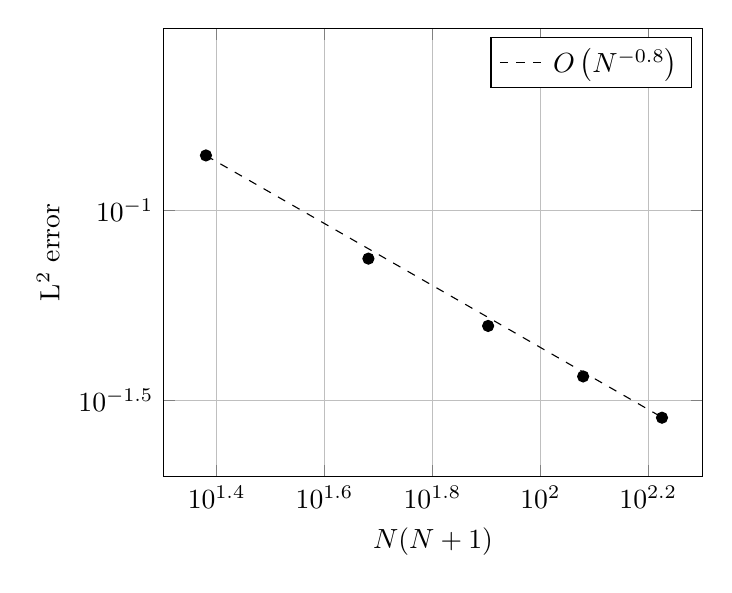
\begin{tikzpicture}
  \begin{axis}[
    %width=0.9\textwidth,
    %height=0.9\textwidth,
    grid=major,
    xlabel={$N(N+1)$},
    ylabel={L$^2$ error},
  	xmode=log,
  	ymode=log,
  	xmin=20,xmax=200,
  	ymin=.02,ymax=0.3,
  	]
\addplot[dashed, black] table[row sep=crcr] {
24 0.139 \\
48 0.0792 \\
80 0.0523 \\
120 0.0376 \\
168 0.0286 \\};
\addlegendentry{$O \left(\text{N}^{-0.8} \right)$}

\addplot[mark=*, mark size=2, draw=black, mark options={solid, fill=black}, only marks] table[row sep=crcr] {
24 0.13912354 \\
48 0.074601074 \\
80 0.049671141 \\
120 0.03661699 \\
168 0.028534338 \\};


  \end{axis}
\end{tikzpicture}
\caption{Accuracy of solutions for the number of directions in a $S_N$ angular quadrature order using $p=2$, on an orthogonal mesh.}
\label{fig:RZGleicherp2g0r1}
\end{figure}
%
It is clear that there is a dependence of the spatial error upon the angular discretization order.


%%%%%%%%%%%%%%%%%%%%%%%%%%%%%%%%%%%%%%%
\subsubsection{Spatial Convergence Studies}
\label{sec:RZSpatialConvergenceStudy}
We perform two spatial convergence studies here, both in \RZ\ geometry. First, we use a smooth manufactured solution to demonstrate optimal convergence rates to compare with the literature in Section~\ref{sec:MMSBailey}. Then, in Section~\ref{sec:DiscontMMS}, we solve a MMS problem that is only a function of space but contains discontinuities in the first-derivative to demonstrate a regularity constrained convergence rate.

%%%%%%%%%%%%%%%%%%%%%%%%%%%%%%%%%%%%%%%
\subsubsubsection{Smooth Manufactured Solution}
\label{sec:MMSBailey}
Bailey et al.~\cite{BaileyDFEMCylindrical} performed this first spatial convergence study and showed $2^\text{nd}$-order convergence using piece-wise linear DFEM (PWLD) and bilinear DFEM (BLD) using the manufactured solution
\begin{flalign}
\psi_\text{MMS}(r,z) & = (\sin(\pi r)+1-r) \sin(\pi z).
\label{eq:MMSBailey}
\end{flalign}

\noindent We obtain the analytical source $S_0$ that gives the exact manufactured solution by inserting Equation~\ref{eq:MMSBailey} into the \RZ\ transport equation
\begin{multline}
\mu \frac{\partial}{\partial r} \left[(\sin(\pi r)+1-r) \sin(\pi z) \right] + \frac{\mu}{r} \left[(\sin(\pi r)+1-r) \sin(\pi z) \right] \\
+ \xi \frac{\partial}{\partial z} \left[(\sin(\pi r)+1-r) \sin(\pi z) \right] - \frac{\mu}{r} \left[(\sin(\pi r)+1-r) \sin(\pi z) \right] \\
- \frac{\eta}{r} \frac{\partial}{\partial \omega} \left[(\sin(\pi r)+1-r) \sin(\pi z) \right] + \sigma_t\ \left[(\sin(\pi r)+1-r) \sin(\pi z) \right] \\
= \sigma_s\ (\sin(\pi r)+1-r) \sin(\pi z) + \frac{1}{2 \pi} S_0,
\end{multline}

\noindent where
\begin{flalign}
\phi_\text{MMS} & = \int_{2 \pi} \psi_{MMS}\ d \Omega \\
& = 2 \pi (\sin(\pi r)+1-r) \sin(\pi z).
\end{flalign}

\noindent Given,
\begin{flalign}
\frac{\partial}{\partial r} \left[(\sin(\pi r)+1-r) \sin(\pi z) \right] & = \pi \cos(\pi r) \sin(\pi z), \\
\frac{\partial}{\partial z} \left[(\sin(\pi r)+1-r) \sin(\pi z) \right] & = \pi (\sin(\pi r)+1-r) \cos(\pi z),
\end{flalign}

\noindent and
\begin{flalign}
\frac{\partial \psi_\text{MMS}}{\partial \omega} & = 0,
\end{flalign}

\noindent we obtain the analytical source for the manufactured solution
\begin{multline}
S_0 = 2 \pi \left[\mu \pi \cos(\pi r) \sin(\pi z) + \xi \pi (\sin(\pi r)+1-r) \cos(\pi z) \right. \\
\left. + \left(\sigma_t - \sigma_s \right) (\sin(\pi r)+1-r) \sin(\pi z) \right].
\end{multline}

We solve this using $\sigma_t = 3 \text{ cm}^{-1}$ and $\sigma_s=0.9999 \sigma_t$. We solved this same problem using $p=\{1,2,4,6,8\}$ on an orthogonal and $2^\text{nd}$-order curved mesh using $S_8$ level-symmetric angular quadrature. We set the incident angular flux to $\psi_\text{MMS}$ of Equation~\ref{eq:MMSBailey}. Figure~\ref{fig:RZBaileyS4O2R2D2} shows the $p=2$ solution on a $2^\text{nd}$-order mesh.

\begin{figure}[!htb]
\centering
\includegraphics[scale=0.3]{../../Research/graphics/RZBaileyS4O2R2D2}
\caption{MMS solution to Equation~\ref{eq:MMSBailey}.}
\label{fig:RZBaileyS4O2R2D2}
\end{figure}

The spatial convergence study performed by Bailey et al.~\cite{BaileyDFEMCylindrical} demonstrated $2^\text{nd}$-order converge for their $1^\text{st}$-order methods. Figures~\ref{fig:RZBaileyS4O2R2D2Ortho} and~\ref{fig:RZBaileyS4O2R2D22Mesh} demonstrate $O(p+1)$ convergence on an orthogonal mesh and $2^\text{nd}$-order mesh, respectively.
%
\begin{figure}[!htb]
\centering
\begin{subfigure}[b]{0.6\textwidth}
\footnotesize
\centering
\begin{tikzpicture}
  \begin{axis}[
    width=0.9\textwidth,
    %height=0.9\textwidth,
    grid=major,
    xlabel={$\sqrt{\text{N}_\text{unknowns}}$},
    ylabel={L$^2$ error},
  	xmode=log,
  	ymode=log,
  	xmin=8,xmax=1e3,
  	ymin=1e-16,ymax=1e1,
  	legend style={at={(1.2,1.0)},anchor=north east},
  	]
\
\addplot[mark=*, only marks, mark size=2, draw=black, mark options={solid, fill=black}] table [x=un1, y=fe1]{../../Research/graphics/RZBaileyMMSS4D0.dat};
\addlegendentry{$p=1$}
\addplot[mark=triangle*, only marks, mark size=3, draw=red, mark options={solid, fill=red}] table [x=un2, y=fe2]{../../Research/graphics/RZBaileyMMSS4D0.dat};
\addlegendentry{$p=2$}
\addplot[mark=square*, only marks, mark size=2, draw=blue, mark options={solid, fill=blue}] table [x=un4, y=fe4]{../../Research/graphics/RZBaileyMMSS4D0.dat};
\addlegendentry{$p=4$}
\addplot[mark=diamond*, only marks, mark size=3, draw=magenta, mark options={solid, fill=magenta}] table [x=un6, y=fe6]{../../Research/graphics/RZBaileyMMSS4D0.dat};
\addlegendentry{$p=6$}
\addplot[mark=star, only marks, mark size=3, draw=orange, mark options={solid, fill=orange}] table [x=un8, y=fe8]{../../Research/graphics/RZBaileyMMSS4D0.dat};
\addlegendentry{$p=8$}

\addplot[black, dashed] table[row sep=crcr] {
8 0.0411 \\
256 1.7075e-06 \\};
\addlegendentry{$O(N^{-2.9})$}
\addplot[red, dashed] table[row sep=crcr] {
12 0.003808954 \\
384 2.0477e-08 \\};
\addlegendentry{$O(N^{-3.5})$}
\addplot[blue, dashed] table[row sep=crcr] {
20	7.90E-06 \\
320	2.1103e-12 \\};
\addlegendentry{$O(N^{-5.5})$}

\addplot[magenta, dashed] table[row sep=crcr] {
28	8.2402E-09 \\
224	1.6475e-15 \\};
\addlegendentry{$O(N^{-7.4})$}

  \end{axis}
\end{tikzpicture}
\caption{Orthogonal quadrilateral mesh.}
\label{fig:RZBaileyS4O2R2D2Ortho}
\end{subfigure}
\begin{subfigure}[b]{0.6\textwidth}
\centering
\footnotesize
\begin{tikzpicture}
  \begin{axis}[
    width=0.9\textwidth,
    %height=0.9\textwidth,
    grid=major,
    xlabel={$\sqrt{\text{N}_\text{unknowns}}$},
    ylabel={L$^2$ error},
  	xmode=log,
  	ymode=log,
  	xmin=8,xmax=1e3,
  	ymin=1e-16,ymax=1e1,
  	legend style={at={(1.2,1.0)},anchor=north east},
  	]
\addplot[mark=*, only marks, mark size=2, draw=black, mark options={solid, fill=black}] table [x=un1, y=fe1]{../../Research/graphics/RZBaileyMMSS4D2.dat};
\addlegendentry{$p=1$}
\addplot[mark=triangle*, only marks, mark size=3, draw=red, mark options={solid, fill=red}] table [x=un2, y=fe2]{../../Research/graphics/RZBaileyMMSS4D2.dat};
\addlegendentry{$p=2$}
\addplot[mark=square*, only marks, mark size=2, draw=blue, mark options={solid, fill=blue}] table [x=un4, y=fe4]{../../Research/graphics/RZBaileyMMSS4D2.dat};
\addlegendentry{$p=4$}
\addplot[mark=diamond*, only marks, mark size=3, draw=magenta, mark options={solid, fill=magenta}] table [x=un6, y=fe6]{../../Research/graphics/RZBaileyMMSS4D2.dat};
\addlegendentry{$p=6$}
\addplot[mark=star, only marks, mark size=3, draw=orange, mark options={solid, fill=orange}] table [x=un8, y=fe8]{../../Research/graphics/RZBaileyMMSS4D2.dat};
\addlegendentry{$p=8$}

\addplot[black, dashed] table[row sep=crcr] {
8 0.097107389 \\
256 8.7077e-06 \\};
\addlegendentry{$O(N^{-2.7})$}
\addplot[red, dashed] table[row sep=crcr] {
12 0.007449226 \\
384 4.5213e-08 \\};
\addlegendentry{$O(N^{-3.5})$}
\addplot[blue, dashed] table[row sep=crcr] {
20	6.91E-05 \\
320	1.5286e-11 \\};
\addlegendentry{$O(N^{-5.5})$}

\addplot[magenta, dashed] table[row sep=crcr] {
28	8.13E-07 \\
224	3.8152e-14 \\};
\addlegendentry{$O(N^{-8.1})$}

\addplot[orange, dashed] table[row sep=crcr] {
36	3.11E-09 \\
144	9.7034e-15 \\};
\addlegendentry{$O(N^{-9.1})$}

  \end{axis}
\end{tikzpicture}
\caption{$2^\text{nd}$-order curved mesh.}
\label{fig:RZBaileyS4O2R2D22Mesh}
\end{subfigure}
\caption{L$^2$-norm of the errors from the manufactured solution and reference lines computed from a least squares fit, where $N_\text{unknowns}~=~N_\text{cells}(p~+~1)^2$.}
\end{figure}
%
Reference lines calculated by a least squares fit are also provided for comparison. These results have been reproduced from Woods and Palmer~\cite{Woods2018RZJCTT}.

Increasing the number of unknowns reduces the error in all cases. For a given finite element order, refining the mesh reduces the error. For a given mesh refinement, the error is smaller for higher-order finite elements. In general, the error values on the curved mesh are larger than corresponding error values on the orthogonal mesh.

\FloatBarrier

%%%%%%%%%%%%%%%%%%%%%%%%%%%%%%%%%%%%%%%
\subsubsubsection{Reduced Regularity Manufactured Solution}
\label{sec:DiscontMMS}
We subsequently looked at the manufactured solution
\begin{flalign}
\psi_\text{MMS} & =
\begin{cases}
1.0 + 4.0 r, & 0 \leq r < 0.33 \\
3.31 - 3.0 r, & 0.33 \leq r < 0.66 \\
2.32 - 1.5 r, & r \leq 1.0
\end{cases},
\label{eq:RZMMSDiscontR}
\end{flalign}

\noindent that is continuous in $\psi(r,z)$, but discontinuous in $\partial_r \psi$. The solution, shown in Figure~\ref{fig:RZMMSDiscontRp2S12g2r3}, was solved using $1^\text{st}$- and $2^\text{nd}$-order finite elements (i.e., $p=1$ and $p=2$, respectively), $S_{12}$ level-symmetric angular quadrature, on a $2^\text{nd}$-order mesh.
%
\begin{figure}[!htb]
\centering
\includegraphics[scale=0.3,trim={50pt 160pt 60pt 50pt},clip]{../../Research/graphics/RZDiscontRp2S12g2r3}
\caption{DGFEM scalar flux solution to Equation~\ref{eq:RZMMSDiscontR}.}
\label{fig:RZMMSDiscontRp2S12g2r3}
\end{figure}
%
We refined the mesh sequentially and plotted the errors as a function of the square root of the number of unknowns in the spatial domain in Figure~\ref{fig:RZMMSDiscontRp2S12g2Errors}.
%
\begin{figure}[!htb]
\centering
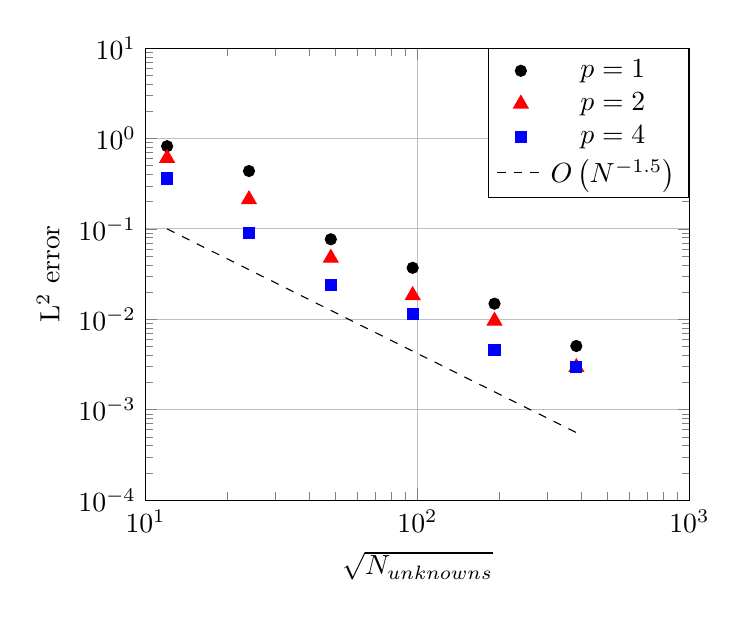
\begin{tikzpicture}
  \begin{axis}[
    width=0.7\textwidth,
    %height=0.9\textwidth,
    grid=major,
    xlabel={$\sqrt{\text{N}_\text{unknowns}}$},
    ylabel={L$^2$ error},
  	xmode=log,
  	ymode=log,
  	xmin=10,xmax=1e3,
  	ymin=1e-4,ymax=1e1,
  	legend style={at={(1.0,1.0)},anchor=north east},
  	]

\addplot[mark=*, only marks, mark size=2, draw=black, mark options={solid, fill=black}] table[row sep=crcr] {
12 0.822493 \\
24 0.43734036 \\
48 0.076831588 \\
96 0.037120875 \\
192 0.014887499 \\
384 0.0050662591 \\};
\addlegendentry{$p=1$}
\addplot[mark=triangle*, mark size=3, only marks, draw=red, mark options={solid, fill=red}] table[row sep=crcr] {
12 0.60652325 \\
24 0.21194424 \\
48 0.047687556 \\
96 0.018428546 \\
192 0.009601399 \\
384 0.0029490701 \\};
\addlegendentry{$p=2$}
\addplot[mark=square*, only marks, mark size=2, draw=blue, mark options={solid, fill=blue}] table[row sep=crcr] {
12 0.36159159 \\
24 0.090767945 \\
48 0.02399935 \\
96 0.011502376 \\
192 0.0045548581 \\
384 0.0029490701 \\};
\addlegendentry{$p=4$}

\addplot[dashed, black] table[row sep=crcr] {
12 0.1 \\
384 5.5820e-04 \\};
\addlegendentry{$O \left(\text{N}^{-1.5} \right)$}

  \end{axis}
\end{tikzpicture}
\caption{L$^2$-norm of the errors from the manufactured solution and reference line, where $N_\text{unknowns}~=~N_\text{cells}(p~+~1)^2$.}
\label{fig:RZMMSDiscontRp2S12g2Errors}
\end{figure}
%
We observe there is a degradation in the spatial convergence rate compared to the smooth (infinitely differentiable) manufactured solution. The analysis by Asadzadeh~\cite{Asadzadeh2DAnalysis} predicts the spatial convergence rate to be as low as $O(1/2)$ or $O(3/2)$ for solutions that have less regularity (i.e., fewer continuous derivatives). We observe the $O(3/2)$ spatial convergence rate for this problem with discontinuous derivatives.

We solved this problem again on an orthogonal mesh with the discontinuities aligned with the mesh surfaces. This restores the spatial convergence rates to the $O(p+1)$ as with a smooth solution. This trivial result is not shown.

\FloatBarrier

%%%%%%%%%%%%%%%%%%%%%%%%%%%%%%%%%%%%%%%
\subsubsection{Spherical Symmetry Preservation}
\label{sec:RZSphericalSymmetry}
Numerically solving the radiation transport equation in \RZ\ geometry for a spherically shaped problem using spherical geometry is a very reasonable idea. However, it is also necessary to solve a spherical problem using cylindrical geometry. One particular application of the transport equation is coupling it to the hydrodynamics equations to solve radiation-hydrodynamics problems. Numerical modeling hydrodynamics problems in cylindrical geometry is common~\cite{DobrevHOAxisymmetric} so we too must demonstrate the ability to model spherical problems using cylindrical geometry.
We want \RZ\ geometry to solve and preserve 1-dimensional spherical solutions. We use MMS to solve a 1-D spherical problem using the \RZ\ geometry spatial discretization.

We evaluate the relative asymmetry by calculating the averages of all nodes at each $\rho=\sqrt{r^2+z^2}$ value and
\begin{flalign}
\phi_\text{asym} (\rho, \theta) & = \frac{\phi_\text{code}(\rho, \theta) - \phi_\text{avg}(\rho)}{\phi_\text{avg}(\rho)},
\label{eq:RelativeAsymmetry}
\end{flalign}
%
\noindent where
\begin{flalign}
\phi_\text{avg}(\rho) & = \frac{1}{N_\text{nodes}(\rho)} \sum_{i=1}^{N_\text{nodes}(\rho)} \phi(\rho,\theta_i)
\end{flalign}
%
\noindent is the average scalar flux at all nodes at the same spherical radius $\rho$.

The three traditional coordinate systems are Cartesian, cylindrical, and spherical. It is straight forward to describe a spatial position using any one of them. However, challenges arise when spatially discretizing. Specifically, angular derivatives arise inside the streaming term in cylindrical and spherical geometries. Cylindrical geometry may be used in lieu of spherical coordinates to describe a spherical problem and is performed this way in some hydrodynamics calculations~\cite{DobrevHOAxisymmetric}. In this section, we demonstrate the use of \RZ\ geometry to preserve a 1-D spherical solution.

Previously, two papers demonstrated spherical modeling of the radiation field using \RZ\ geometry. Brunner et al.~\cite{BrunnerSphericalsymmetry} performed this analysis for the diffusion equation with an incident boundary condition on the outside of the moderately scattering homogeneous sphere with zero source. Their results were mixed whether each discretization method preserved accuracy of their analytical solution and preserved the axisymmetry. Chanland and Sama~\cite{Chaland2016SphericalSymmetry} performed an analysis with the time-dependent transport equation with an initial source at the center of a void. They concluded that the \SN\ method produces ray-effects in the void and their unique angular discretization qualitatively preserved axisymmetry. While there are applications for considering radiation propagation through a voided region, this current work focuses on material problems.

We use the method of manufactured solutions (MMS) with the manufactured solution
\begin{flalign}
\psi_\text{MMS}(r,z) & = \rho = \sqrt{r^2+z^2}.
\label{eq:RZMMSLinearRho}
\end{flalign}
%
This solution is linear in the 1-D spherical coordinate $\rho$. We obtain the analytical source $S_0$ that gives the exact manufactured solution by inserting Equation~\ref{eq:RZMMSLinearRho} into the \RZ\ transport equation
\begin{flalign}
\mu \frac{\partial \rho}{\partial r} + \frac{\mu}{r} \rho + \xi \frac{\partial \rho}{\partial z} - \frac{\mu}{r} \rho - \frac{\eta}{r} \frac{\partial \rho}{\partial \omega} + \sigma_t\ \rho & = \sigma_s\ \rho + \frac{1}{2 \pi} S_0, \\
\mu \frac{\partial \rho}{\partial r} + \xi \frac{\partial \rho}{\partial z} - \frac{\eta}{r} \frac{\partial \rho}{\partial \omega} + \sigma_t\ \rho & = \sigma_s\ \rho + \frac{1}{2 \pi} S_0
\end{flalign}

\noindent where
\begin{flalign}
\phi_\text{MMS} & = \int_{2 \pi} \psi_{MMS}\ d \Omega \\
& = 2 \pi \rho.
\end{flalign}

\noindent Given,
\begin{flalign}
\frac{\partial \rho}{\partial r} & = \frac{r}{\sqrt{r^2+z^2}}, \\
\frac{\partial \rho}{\partial z} & = \frac{z}{\sqrt{r^2+z^2}},
\end{flalign}

\noindent and
\begin{flalign}
\frac{\partial \rho}{\partial \omega} & = 0,
\end{flalign}

\noindent we obtain the analytical source for the manufactured solution
\begin{flalign}
S_0 & = 2 \pi \left(\frac{\mu\ r}{\sqrt{r^2+z^2}} + \frac{\xi\ z}{\sqrt{r^2+z^2}} - \sigma_s\ \sqrt{r^2+z^2} \right).
\end{flalign}

There are numerous discretizations that may impact the solution to this MMS problem, including: angular discretization order, finite element order, spatial mesh refinement, and mesh curvature. We perform numerical tests to investigate the impact of each of these discretizations have on preserving spherical symmetry. Additionally, we perform several cross-correlation tests for a few of these. We solve this MMS problem on a LO mesh and a HO ($2^\text{nd}$-order) mesh in Sections~\ref{subsec:LOMesh}~and~\ref{subsec:HOMesh}, respectively. Within these sections, we solve this MMS problem using $S_N$ level symmetric angular quadrature with $N=\{4,6,8,10,12\}$, for finite element orders $p=\{1,2,4\}$, and various levels of mesh refinement. These discretization approximations (mesh and mesh order, $S_N$ order, and finite element order) contribute to the asymmetry of the solution. We study each one individually to characterize the effects of each on the asymmetry. The problem has physical parameters $\sigma_t=5.0$ and $\sigma_a=2.0$. We summarize all of these results and make some concluding remarks in Section~\ref{sub:AxiSymSummaryDiscussion}.

An example scalar flux solution is shown in Figure~\ref{fig:RZASMMSLinearRhoBrunnerp1S8g2r5PhiNoContour}.
%
\begin{figure}[!htb]
\includegraphics[scale=0.4]{../../Research/graphics/Axisymmetry/RZASMMSLinearRhoBrunner/p1S8g2r5PhiNoContour}
\caption{Example scalar flux solution using $1^\text{st}$-order finite elements, $S_8$ level-symmetric angular quadrature, $2^\text{nd}$-order mesh, and refined  mesh with 8128 mesh zones.}
\label{fig:RZASMMSLinearRhoBrunnerp1S8g2r5PhiNoContour}
\end{figure}
%
The solution appears smooth in all spherical radial directions.

%%%%%%%%%%%%%%%%%%%%%%%%%%%%%%%%%%%%%%%
\subsubsubsection{Low-Order Mesh}
\label{subsec:LOMesh}
In this section, we observe the sensitivity of the scalar flux spherical asymmetry to changing the discrete ordinates order, finite element order, and spatial refinement on a low-order mesh. Specifically, a low-order mesh is one that has linear surfaces. The vertices of the low-order meshes used in this section are located in concentric rings of equal $\rho=\sqrt{r^2+z^2}$. The results in this section are organized as follows: comparing the discrete ordinates order for each of $p=\{1,2,4,8\}$, comparing each of $p=\{1,2,4,8\}$ for $S_8$ level symmetric angular quadrature, and mesh refinement studies for each of $p=\{1,4\}$.

Figure~\ref{fig:RZASMMSLinearRhoBrunnerp1g1r2} shows the $\phi_\text{asym}$ values calculated using Equation~\ref{eq:RelativeAsymmetry} for $1^\text{st}$-order finite elements on a $1^\text{st}$-order mesh with 120 zones for several angular quadrature discretizations. The asymmetry is plotted on a log scale. The scale colors assist in demonstrating the qualitative locations of the asymmetries. The yellow region is the least symmetric, red regions have increased symmetry, and blue regions have the most symmetry. The $\phi_\text{asym}$ solution is plotted using the same finite element shape functions as the scalar flux. There is no perceptible gain in symmetry by increasing the angular discretization order. We confirm this by plotting the asymmetry values as a function of the spherical radius (i.e., $\rho=\sqrt{r^2+z^2}$) in Figure~\ref{fig:RZASMMSLinearRhoBrunnerp1g1r2Nodes}. The spherical radial asymmetry solutions are indistinguishable between discrete ordinate orders. The location of the largest asymmetries are near the polar axis (i.e., $r=0$). We observe groupings along the top profile of this figure. These asymmetry values occur along the $z$-axis where the remaining nodal solutions in the problem interior have smaller asymmetries. Moreover, Figure~\ref{fig:RZASMMSLinearRhoBrunnerp1g1r2Accuracy} demonstrates there is no gain in accuracy by increasing the $S_N$ order.

\begin{sidewaysfigure}[!htb]
\centering
\begin{subfigure}{0.33\textwidth}
\includegraphics[scale=0.3,trim={50pt 70pt 320pt 45pt},clip]{../../Research/graphics/Axisymmetry/RZASMMSLinearRhoBrunner/p1S4g1r2}
\caption{$S_4$.}
\end{subfigure}%
%\begin{subfigure}{0.2\textwidth}
%\includegraphics[scale=0.25,trim={50pt 70pt 320pt 45pt},clip]{../../Research/graphics/Axisymmetry/RZASMMSLinearRhoBrunner/p1S6g1r2}
%\caption{$S_6$.}
%\end{subfigure}%
\begin{subfigure}{0.33\textwidth}
\includegraphics[scale=0.3,trim={50pt 70pt 320pt 45pt},clip]{../../Research/graphics/Axisymmetry/RZASMMSLinearRhoBrunner/p1S8g1r2}
\caption{$S_8$.}
\end{subfigure}%
%\begin{subfigure}{0.2\textwidth}
%\includegraphics[scale=0.25,trim={50pt 70pt 320pt 45pt},clip]{../../Research/graphics/Axisymmetry/RZASMMSLinearRhoBrunner/p1S10g1r2}
%\caption{$S_{10}$.}
%\end{subfigure}%
\begin{subfigure}{0.33\textwidth}
\includegraphics[scale=0.3,trim={50pt 70pt 320pt 45pt},clip]{../../Research/graphics/Axisymmetry/RZASMMSLinearRhoBrunner/p1S12g1r2}
\caption{$S_{12}$.}
\end{subfigure}
\caption{Relative asymmetry for $1^\text{st}$-order finite elements on a $1^\text{st}$-order mesh for given order of level-symmetric angular quadrature.}
\label{fig:RZASMMSLinearRhoBrunnerp1g1r2}
\end{sidewaysfigure}

\begin{figure}[!htb]
\centering
\includegraphics[scale=1]{./graphics/RZASMMSLinearRhoBrunnerp1g1r2.pdf}
\caption{Measure of the asymmetry for each finite element node for the given level-symmetric angular quadrature order for $1^\text{st}$-order DFEM and $1^\text{st}$-order mesh with 120 zones (see Figure~\ref{fig:RZASMMSLinearRhoBrunnerp1g1r2}).}
\label{fig:RZASMMSLinearRhoBrunnerp1g1r2Nodes}
\end{figure}

\begin{figure}[!htb]
\centering
\begin{tikzpicture}
  \begin{axis}[
    %width=0.9\textwidth,
    %height=0.9\textwidth,
    grid=major,
    xlabel={$S_N$},
    ylabel={L$^2$ error},
  	%xmode=log,
  	ymode=log,
  	xmin=4,xmax=12,
  	ymin=1e-3,ymax=1e-2,
  	]
\addplot[mark=*, mark size=2, draw=black, mark options={solid, fill=black}] table[row sep=crcr] {
4 0.0020941929 \\
6 0.0020971511 \\
8 0.0021251254 \\
10 0.0021502437 \\
12 0.0021700218 \\};

  \end{axis}
\end{tikzpicture}
\caption{Accuracy of solutions for given angular quadrature using $p=1$ on a $1^\text{st}$-order mesh with 120 zones.}
\label{fig:RZASMMSLinearRhoBrunnerp1g1r2Accuracy}
\end{figure}

\FloatBarrier

Figure~\ref{fig:RZASMMSLinearRhoBrunnerp2g1r2} shows the $\phi_\text{asym}$ values calculated using Equation~\ref{eq:RelativeAsymmetry} for $2^\text{nd}$-order finite elements on a $1^\text{st}$-order mesh with 120 zones for several angular quadrature discretizations. The asymmetry is plotted on a log scale. The scale colors assist in demonstrating the qualitative locations of the asymmetries. The yellow region is the least symmetric, red regions have increased symmetry, and blue regions have the most symmetry. The $\phi_\text{asym}$ solution is plotted using the same finite element shape functions as the scalar flux. There is a little perceptible gain in symmetry (indicated by more blue area) on the periphery by increasing the angular discretization order. However, plotting the asymmetry values as a function of the spherical radius (i.e., $\rho=\sqrt{r^2+z^2}$) in Figure~\ref{fig:RZASMMSLinearRhoBrunnerp2g1r2Nodes} shows that there may not actually be any symmetry gains --- the spherical radial asymmetry solutions are indistinguishable between discrete ordinate orders. The asymmetries are predominantly located near the origin (i.e., $\rho=\sqrt{r^2+z^2}=0$). Moreover, Figure~\ref{fig:RZASMMSLinearRhoBrunnerp2g1r2Accuracy} demonstrates there is no gain in accuracy by increasing the $S_N$ order.

\begin{sidewaysfigure}[!htb]
\centering
\begin{subfigure}{0.33\textwidth}
\includegraphics[scale=0.3,trim={50pt 70pt 320pt 45pt},clip]{../../Research/graphics/Axisymmetry/RZASMMSLinearRhoBrunner/p2S4g1r2}
\caption{$S_4$.}
\end{subfigure}%
%\begin{subfigure}{0.2\textwidth}
%\includegraphics[scale=0.25,trim={50pt 70pt 320pt 45pt},clip]{../../Research/graphics/Axisymmetry/RZASMMSLinearRhoBrunner/p2S6g1r2}
%\caption{$S_6$.}
%\end{subfigure}%
\begin{subfigure}{0.33\textwidth}
\includegraphics[scale=0.3,trim={50pt 70pt 320pt 45pt},clip]{../../Research/graphics/Axisymmetry/RZASMMSLinearRhoBrunner/p2S8g1r2}
\caption{$S_8$.}
\end{subfigure}%
%\begin{subfigure}{0.2\textwidth}
%\includegraphics[scale=0.25,trim={50pt 70pt 320pt 45pt},clip]{../../Research/graphics/Axisymmetry/RZASMMSLinearRhoBrunner/p2S10g1r2}
%\caption{$S_10$.}
%\end{subfigure}%
\begin{subfigure}{0.33\textwidth}
\includegraphics[scale=0.3,trim={50pt 70pt 320pt 45pt},clip]{../../Research/graphics/Axisymmetry/RZASMMSLinearRhoBrunner/p2S12g1r2}
\caption{$S_{12}$.}
\end{subfigure}
\caption{Relative asymmetry for $2^\text{st}$-order finite elements on a $1^\text{st}$-order mesh for given order of level-symmetric angular quadrature.}
\label{fig:RZASMMSLinearRhoBrunnerp2g1r2}
\end{sidewaysfigure}

\begin{figure}[!htb]
\centering
\includegraphics[scale=1]{./graphics/RZASMMSLinearRhoBrunnerp2g1r2.pdf}
\caption{Measure of the asymmetry for each finite element node for the given level-symmetric angular quadrature order for $2^\text{nd}$-order DFEM and $1^\text{st}$-order mesh with 120 zones (see Figure~\ref{fig:RZASMMSLinearRhoBrunnerp2g1r2}).}
\label{fig:RZASMMSLinearRhoBrunnerp2g1r2Nodes}
\end{figure}

\begin{figure}[!htb]
\centering
\begin{tikzpicture}
  \begin{axis}[
    %width=0.9\textwidth,
    %height=0.9\textwidth,
    grid=major,
    xlabel={$S_N$},
    ylabel={L$^2$ error},
  	%xmode=log,
  	ymode=log,
  	xmin=4,xmax=12,
  	ymin=1e-5,ymax=1e-4,
  	]
\addplot[mark=*, mark size=2, draw=black, mark options={solid, fill=black}] table[row sep=crcr] {
4 4.2240043e-05 \\
6 4.183292e-05 \\
8 4.1616786e-05 \\
10 4.1382778e-05 \\
12 4.1162625e-05 \\};

  \end{axis}
\end{tikzpicture}
\caption{Accuracy of solutions for given angular quadrature using $p=2$ on a $1^\text{st}$-order mesh with 120 zones.}
\label{fig:RZASMMSLinearRhoBrunnerp2g1r2Accuracy}
\end{figure}

\FloatBarrier

Figure~\ref{fig:RZASMMSLinearRhoBrunnerp4g1r2} shows the $\phi_\text{asym}$ values calculated using Equation~\ref{eq:RelativeAsymmetry} for $4^\text{th}$-order finite elements on a $1^\text{st}$-order mesh with 120 zones for several angular quadrature discretizations. The asymmetry is plotted on a log scale. The scale colors assist in demonstrating the qualitative locations of the asymmetries. The yellow region is the least symmetric, red regions have increased symmetry, and blue regions have the most symmetry. The $\phi_\text{asym}$ solution is plotted using the same finite element shape functions as the scalar flux. There is no perceptible gain in symmetry by increasing the angular discretization order. This is confirmed by plotting the asymmetry values as a function of the spherical radius (i.e., $\rho=\sqrt{r^2+z^2}$) in Figure~\ref{fig:RZASMMSLinearRhoBrunnerp4g1r2Nodes}. Unlike Figure~\ref{fig:RZASMMSLinearRhoBrunnerp2g1r2}, the asymmetry of the scalar flux appears to be a function of the spherical radius, $\rho$. Moreover, Figure~\ref{fig:RZASMMSLinearRhoBrunnerp4g1r2Accuracy} demonstrates there is no gain in accuracy by increasing the $S_N$ order.

\begin{sidewaysfigure}[!htb]
\centering
\begin{subfigure}{0.33\textwidth}
\includegraphics[scale=0.3,trim={50pt 70pt 320pt 45pt},clip]{../../Research/graphics/Axisymmetry/RZASMMSLinearRhoBrunner/p4S4g1r2}
\caption{$S_4$.}
\end{subfigure}%
%\begin{subfigure}{0.2\textwidth}
%\includegraphics[scale=0.25,trim={50pt 70pt 320pt 45pt},clip]{../../Research/graphics/Axisymmetry/RZASMMSLinearRhoBrunner/p4S6g1r2}
%\caption{$S_6$.}
%\end{subfigure}%
\begin{subfigure}{0.33\textwidth}
\includegraphics[scale=0.3,trim={50pt 70pt 320pt 45pt},clip]{../../Research/graphics/Axisymmetry/RZASMMSLinearRhoBrunner/p4S8g1r2}
\caption{$S_8$.}
\end{subfigure}%
%\begin{subfigure}{0.2\textwidth}
%\includegraphics[scale=0.25,trim={50pt 70pt 320pt 45pt},clip]{../../Research/graphics/Axisymmetry/RZASMMSLinearRhoBrunner/p4S10g1r2}
%\caption{$S_{10}$.}
%\end{subfigure}%
\begin{subfigure}{0.33\textwidth}
\includegraphics[scale=0.3,trim={50pt 70pt 320pt 45pt},clip]{../../Research/graphics/Axisymmetry/RZASMMSLinearRhoBrunner/p4S12g1r2}
\caption{$S_{12}$.}
\end{subfigure}
\caption{Relative asymmetry for $4^\text{st}$-order finite elements on a $1^\text{st}$-order mesh for given order of level-symmetric angular quadrature.}
\label{fig:RZASMMSLinearRhoBrunnerp4g1r2}
\end{sidewaysfigure}

\begin{figure}[!htb]
\centering
\includegraphics[scale=1]{./graphics/RZASMMSLinearRhoBrunnerp4g1r2.pdf}
\caption{Measure of the asymmetry for each finite element node for the given level-symmetric angular quadrature order for $4^\text{th}$-order DFEM and $1^\text{st}$-order mesh with 120 zones (see Figure~\ref{fig:RZASMMSLinearRhoBrunnerp4g1r2}).}
\label{fig:RZASMMSLinearRhoBrunnerp4g1r2Nodes}
\end{figure}

\begin{figure}[!htb]
\centering
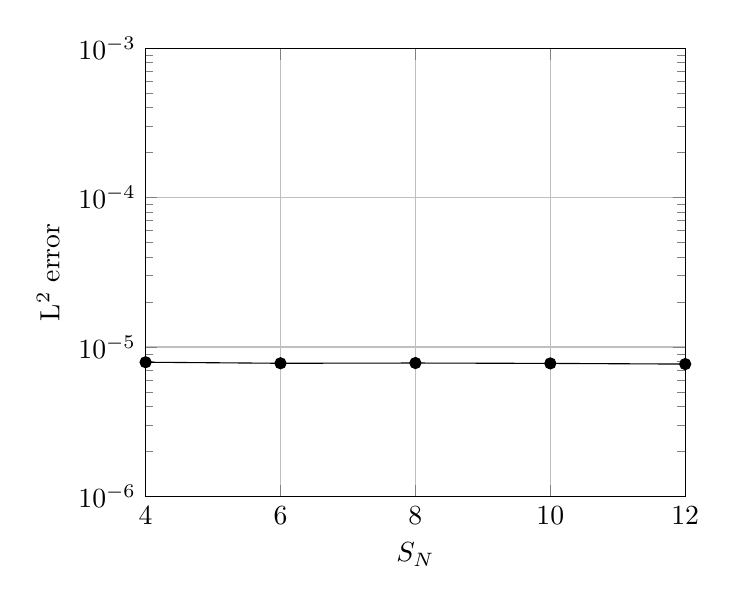
\begin{tikzpicture}
  \begin{axis}[
    %width=0.9\textwidth,
    %height=0.9\textwidth,
    grid=major,
    xlabel={$S_N$},
    ylabel={L$^2$ error},
  	%xmode=log,
  	ymode=log,
  	xmin=4,xmax=12,
  	ymin=1e-6,ymax=1e-3,
  	]
\addplot[mark=*, mark size=2, draw=black, mark options={solid, fill=black}] table[row sep=crcr] {
4 7.9142016e-06 \\
6 7.7873045e-06 \\
8 7.8171296e-06 \\
10 7.7723314e-06 \\
12 7.6917507e-06 \\};

  \end{axis}
\end{tikzpicture}
\caption{Accuracy of solutions for given angular quadrature using $p=4$ on a $1^\text{st}$-order mesh with 120 zones.}
\label{fig:RZASMMSLinearRhoBrunnerp4g1r2Accuracy}
\end{figure}

\FloatBarrier

Figure~\ref{fig:RZASMMSLinearRhoBrunnerp8g1r2} shows the $\phi_\text{asym}$ values calculated using Equation~\ref{eq:RelativeAsymmetry} for $8^\text{th}$-order finite elements on a $1^\text{st}$-order mesh with 120 zones for several angular quadrature discretizations. The asymmetry is plotted on a log scale. The scale colors assist in demonstrating the qualitative locations of the asymmetries. The yellow region is the least symmetric, red regions have increased symmetry, and blue regions have the most symmetry. The $\phi_\text{asym}$ solution is plotted using the same finite element shape functions as the scalar flux. There is no perceptible gain in symmetry by increasing the angular discretization order. However, Figure~\ref{fig:RZASMMSLinearRhoBrunnerp8g1r2Nodes} shows there is a slight increase in symmetry from $S_4$ for $\rho \geq 0.7$. Similar to Figure~\ref{fig:RZASMMSLinearRhoBrunnerp4g1r2}, the asymmetry of the scalar flux appears to be a function of the spherical radius, $\rho$. Moreover, Figure~\ref{fig:RZASMMSLinearRhoBrunnerp8g1r2Accuracy} demonstrates there is an increase in accuracy by increasing the finite element order.

\begin{sidewaysfigure}[!htb]
\centering
\begin{subfigure}{0.33\textwidth}
\includegraphics[scale=0.3,trim={50pt 70pt 320pt 45pt},clip]{../../Research/graphics/Axisymmetry/RZASMMSLinearRhoBrunner/p8S4g1r2}
\caption{$S_4$.}
\end{subfigure}%
%\begin{subfigure}{0.2\textwidth}
%\includegraphics[scale=0.25,trim={50pt 70pt 320pt 45pt},clip]{../../Research/graphics/Axisymmetry/RZASMMSLinearRhoBrunner/p8S6g1r2}
%\caption{$S_6$.}
%\end{subfigure}%
\begin{subfigure}{0.33\textwidth}
\includegraphics[scale=0.3,trim={50pt 70pt 320pt 45pt},clip]{../../Research/graphics/Axisymmetry/RZASMMSLinearRhoBrunner/p8S8g1r2}
\caption{$S_8$.}
\end{subfigure}%
%\begin{subfigure}{0.2\textwidth}
%\includegraphics[scale=0.25,trim={50pt 70pt 320pt 45pt},clip]{../../Research/graphics/Axisymmetry/RZASMMSLinearRhoBrunner/p8S10g1r2}
%\caption{$S_{10}$.}
%\end{subfigure}%
\begin{subfigure}{0.33\textwidth}
\includegraphics[scale=0.3,trim={50pt 70pt 320pt 45pt},clip]{../../Research/graphics/Axisymmetry/RZASMMSLinearRhoBrunner/p8S10g1r2}
\caption{$S_{12}$.}
\end{subfigure}
\caption{Relative asymmetry for $8^\text{st}$-order finite elements on a $1^\text{st}$-order mesh for given order of level-symmetric angular quadrature.}
\label{fig:RZASMMSLinearRhoBrunnerp8g1r2}
\end{sidewaysfigure}

\begin{figure}[!htb]
\centering
\includegraphics[scale=1]{./graphics/RZASMMSLinearRhoBrunnerp8g1r2.pdf}
\caption{Measure of the asymmetry for each finite element node for the given level-symmetric angular quadrature order for $8^\text{th}$-order DFEM and $1^\text{st}$-order mesh with 120 zones (see Figure~\ref{fig:RZASMMSLinearRhoBrunnerp8g1r2}).}
\label{fig:RZASMMSLinearRhoBrunnerp8g1r2Nodes}
\end{figure}

\begin{figure}[!htb]
\centering
\begin{tikzpicture}
  \begin{axis}[
    %width=0.9\textwidth,
    %height=0.9\textwidth,
    grid=major,
    xlabel={$S_N$},
    ylabel={L$^2$ error},
  	%xmode=log,
  	ymode=log,
  	xmin=4,xmax=12,
  	ymin=1e-7,ymax=2e-6,
  	]
\addplot[mark=*, mark size=2, draw=black, mark options={solid, fill=black}] table[row sep=crcr] {
4 1.0005222e-06 \\
6 9.7947455e-07 \\
8 9.8658298e-07 \\
10 9.8200156e-07 \\
12 9.6633416e-07 \\};

  \end{axis}
\end{tikzpicture}
\caption{Accuracy of solutions for given angular quadrature using $p=8$ on a $1^\text{st}$-order mesh with 120 zones.}
\label{fig:RZASMMSLinearRhoBrunnerp8g1r2Accuracy}
\end{figure}

\FloatBarrier

Figure~\ref{fig:RZASMMSLinearRhoBrunnerS8g1r2CompareP} shows the $\phi_\text{asym}$ values calculated using Equation~\ref{eq:RelativeAsymmetry} for $p=\{1,2,4\}$ finite elements on a $2^\text{nd}$-order mesh with 120 zones with $S_8$ level-symmetric angular quadrature repeated from Figures~\ref{fig:RZASMMSLinearRhoBrunnerp1g1r2},~\ref{fig:RZASMMSLinearRhoBrunnerp2g1r2},~and~\ref{fig:RZASMMSLinearRhoBrunnerp4g1r2} and plotted on the same scale. Increasing the finite element order provides significant gains in symmetry shown by the reduction in yellow regions and increase in blue regions. We corroborate these results by plotting the asymmetry values as a function of the spherical radius (i.e., $\rho=\sqrt{r^2+z^2}$) in Figure~\ref{fig:RZASMMSLinearRhoBrunnerS8g1r2Nodes}. It is evident that increasing the finite element order provides gains in spherical symmetry. Moreover, Figure~\ref{fig:RZASMMSLinearRhoBrunnerS8g1r2Accuracy} demonstrates there is an increase in accuracy by increasing the finite element order except for $8^\text{th}$-order finite elements.

\begin{sidewaysfigure}[!htb]
\centering
\begin{subfigure}{0.33\textwidth}
\includegraphics[scale=0.3,trim={50pt 70pt 320pt 45pt},clip]{../../Research/graphics/Axisymmetry/RZASMMSLinearRhoBrunner/p1S8g1r2CompP}
\caption{$p=1$.}
\end{subfigure}%
\begin{subfigure}{0.33\textwidth}
\includegraphics[scale=0.3,trim={50pt 70pt 320pt 45pt},clip]{../../Research/graphics/Axisymmetry/RZASMMSLinearRhoBrunner/p2S8g1r2CompP}
\caption{$p=2$.}
\end{subfigure}%
\begin{subfigure}{0.33\textwidth}
\includegraphics[scale=0.3,trim={50pt 70pt 320pt 45pt},clip]{../../Research/graphics/Axisymmetry/RZASMMSLinearRhoBrunner/p4S8g1r2CompP}
\caption{$p=4$.}
\end{subfigure}
\caption{Relative asymmetry for $p=\{1,2,4\}$ finite elements on a $1^\text{st}$-order mesh with 120 zones for $S_8$ level-symmetric angular quadrature.}
\label{fig:RZASMMSLinearRhoBrunnerS8g1r2CompareP}
\end{sidewaysfigure}

\begin{figure}[!htb]
\centering
\includegraphics[scale=1]{./graphics/RZASMMSLinearRhoBrunnerS8g1r2.pdf}
\caption{Measure of the asymmetry for each finite element node for the given finite element order using $S_8$ level-symmetric angular quadrature on a $1^\text{st}$-order mesh with 120 zones (see Figure~\ref{fig:RZASMMSLinearRhoBrunnerS8g1r2CompareP}).}
\label{fig:RZASMMSLinearRhoBrunnerS8g1r2Nodes}
\end{figure}

\begin{figure}[!htb]
\centering
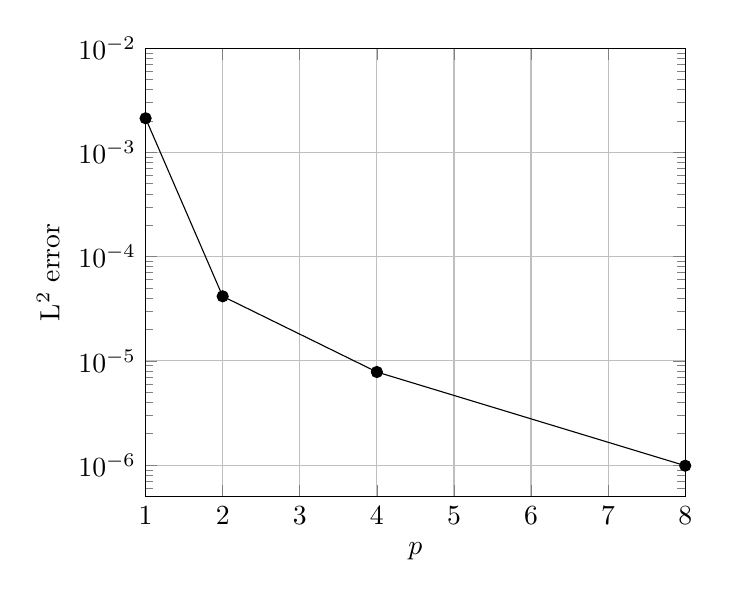
\begin{tikzpicture}
  \begin{axis}[
    %width=0.9\textwidth,
    %height=0.9\textwidth,
    grid=major,
    xlabel={$p$},
    ylabel={L$^2$ error},
  	%xmode=log,
  	ymode=log,
  	xmin=1,xmax=8,
  	ymin=5e-7,ymax=1e-2,
  	]
\addplot[mark=*, mark size=2, draw=black, mark options={solid, fill=black}] table[row sep=crcr] {
1 0.0021251254 \\
2 4.1616786e-05 \\
4 7.8171296e-06 \\
8 9.8658298e-07 \\};

  \end{axis}
\end{tikzpicture}
\caption{Accuracy of solutions for given finite element order using $S_8$ level-symmetric angular quadrature on a $1^\text{st}$-order mesh with 120 zones.}
\label{fig:RZASMMSLinearRhoBrunnerS8g1r2Accuracy}
\end{figure}

\FloatBarrier

We also investigated the symmetry preservation by performing sequential mesh refinements for $p=1$ with $S_8$ level-symmetric angular quadrature. Figures~\ref{fig:RZASMMSLinearRhoBrunnerp1S8g1Part1}~and~\ref{fig:RZASMMSLinearRhoBrunnerp1S8g1Part2} show the first several mesh refinement steps. The asymmetry is plotted on a log scale. The scale colors assist in demonstrating the qualitative locations of the asymmetries. The yellow region is the least symmetric, red regions have increased symmetry, and blue regions have the most symmetry. The $\phi_\text{asym}$ solution is plotted using the same finite element shape functions as the scalar flux. There is some gain (a few orders of magnitude) in symmetry by refining the $1^\text{st}$-order mesh. We observe large regions of $\phi_\text{asym}$ changing from yellow to red through the mesh refinement. Plotting the symmetry values as a function of the spherical radius (i.e., $\rho=\sqrt{r^2+z^2}$) in Figure~\ref{fig:RZASMMSLinearRhoBrunnerp1S8g1Nodes} shows that there is some symmetry gain by refining the mesh. The largest asymmetry magnitude of the scalar flux is near the polar axis (i.e. $r=0$) as previously seen in Figure~\ref{fig:RZASMMSLinearRhoBrunnerp1g1r2}. Moreover, Figure~\ref{fig:RZASMMSLinearRhoBrunnerp1S8g1Accuracy} demonstrates there is an increase in accuracy by refining the spatial mesh.

\begin{sidewaysfigure}[!htb]
\centering
\begin{subfigure}{0.33\textwidth}
\includegraphics[scale=0.3,trim={50pt 70pt 320pt 45pt},clip]{../../Research/graphics/Axisymmetry/RZASMMSLinearRhoBrunner/p1S8g1r0CompR}
\caption{$N_\text{zones}=6$.}
\end{subfigure}%
\begin{subfigure}{0.33\textwidth}
\includegraphics[scale=0.3,trim={50pt 70pt 320pt 45pt},clip]{../../Research/graphics/Axisymmetry/RZASMMSLinearRhoBrunner/p1S8g1r1CompR}
\caption{$N_\text{zones}=28$.}
\end{subfigure}%
\begin{subfigure}{0.33\textwidth}
\includegraphics[scale=0.3,trim={50pt 70pt 320pt 45pt},clip]{../../Research/graphics/Axisymmetry/RZASMMSLinearRhoBrunner/p1S8g1r2CompR}
\caption{$N_\text{zones}=120$.}
\end{subfigure}
\caption{Relative asymmetry for $p=1$ finite elements on a $1^\text{st}$-order mesh for $S_8$ level-symmetric angular quadrature for $N_\text{zones}=\{6,28,120\}$.}
\label{fig:RZASMMSLinearRhoBrunnerp1S8g1Part1}
\end{sidewaysfigure}

\begin{sidewaysfigure}[!htb]
\centering
\begin{subfigure}{0.33\textwidth}
\includegraphics[scale=0.3,trim={50pt 70pt 320pt 45pt},clip]{../../Research/graphics/Axisymmetry/RZASMMSLinearRhoBrunner/p1S8g1r3CompR}
\caption{$N_\text{zones}=496$.}
\end{subfigure}%
\begin{subfigure}{0.33\textwidth}
\includegraphics[scale=0.3,trim={50pt 70pt 320pt 45pt},clip]{../../Research/graphics/Axisymmetry/RZASMMSLinearRhoBrunner/p1S8g1r4CompR}
\caption{$N_\text{zones}=2016$.}
\end{subfigure}%
\begin{subfigure}{0.33\textwidth}
\includegraphics[scale=0.3,trim={50pt 70pt 320pt 45pt},clip]{../../Research/graphics/Axisymmetry/RZASMMSLinearRhoBrunner/p1S8g1r5CompR}
\caption{$N_\text{zones}=8128$.}
\end{subfigure}
\caption{Relative asymmetry for $p=1$ finite elements on a $1^\text{st}$-order mesh for $S_8$ level-symmetric angular quadrature for $N_\text{zones}=\{496,2016,8128\}$; mesh overlay may be removed for clarity.}
\label{fig:RZASMMSLinearRhoBrunnerp1S8g1Part2}
\end{sidewaysfigure}

\begin{figure}[!htb]
\centering
\includegraphics[scale=1]{./graphics/RZASMMSLinearRhoBrunnerp1S8g1.pdf}
\caption{Measure of the asymmetry for each finite element node for $1^\text{th}$-order finite elements using $S_8$ level-symmetric angular quadrature on a $1^\text{st}$-order mesh with various number of zones (see Figures~\ref{fig:RZASMMSLinearRhoBrunnerp1S8g1Part1}-\ref{fig:RZASMMSLinearRhoBrunnerp1S8g1Part2}).}
\label{fig:RZASMMSLinearRhoBrunnerp1S8g1Nodes}
\end{figure}

\begin{figure}[!htb]
\centering
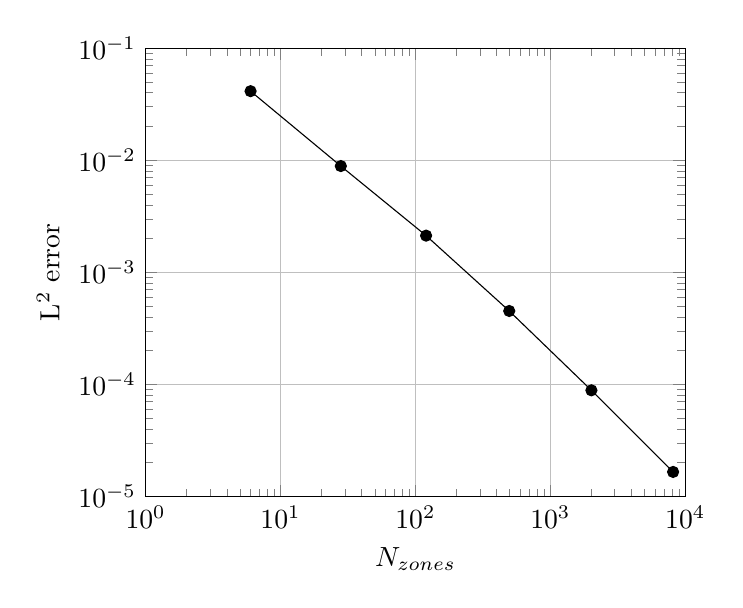
\begin{tikzpicture}
  \begin{axis}[
    %width=0.9\textwidth,
    %height=0.9\textwidth,
    grid=major,
    xlabel={$N_\text{zones}$},
    ylabel={L$^2$ error},
  	xmode=log,
  	ymode=log,
  	xmin=1,xmax=1e4,
  	ymin=1e-5,ymax=1e-1,
  	]
\addplot[mark=*, mark size=2, draw=black, mark options={solid, fill=black}] table[row sep=crcr] {
6 0.041323342 \\
28 0.0088741901 \\
120 0.0021251254 \\
496 0.00045204233 \\
2016 8.8560131e-05 \\
8128 1.6559953e-05 \\};

  \end{axis}\end{tikzpicture}
\caption{Accuracy of solutions for given mesh refinement for $p=1$ using $S_8$ level-symmetric angular quadrature on a $1^\text{st}$-order mesh.}
\label{fig:RZASMMSLinearRhoBrunnerp1S8g1Accuracy}
\end{figure}

\FloatBarrier

We also investigated the symmetry preservation by performing sequential mesh refinements for $p=4$ with $S_8$ level-symmetric angular quadrature. Figures~\ref{fig:RZASMMSLinearRhoBrunnerp4S8g1Part1}~and~\ref{fig:RZASMMSLinearRhoBrunnerp4S8g1Part2} show the first several mesh refinement steps. The asymmetry is plotted on a log scale. The scale colors assist in demonstrating the qualitative locations of the asymmetries. The yellow region is the least symmetric, red regions have increased symmetry, and blue regions have the most symmetry. The $\phi_\text{asym}$ solution is plotted using the same finite element shape functions as the scalar flux. There is tremendous gain (many orders of magnitude) in symmetry by refining the $1^\text{st}$-order mesh. We observe large regions of $\phi_\text{asym}$ changing from yellow to red to blue throughout the mesh refinement. Plotting the symmetry values as a function of the spherical radius (i.e., $\rho=\sqrt{r^2+z^2}$) in Figure~\ref{fig:RZASMMSLinearRhoBrunnerp4S8g1Nodes} confirms the substantial symmetry gain by refining the mesh. The largest asymmetry magnitude of the scalar flux remains near the origin (i.e. $\rho=\sqrt{r^2+z^2}=0$) as previously seen, but also remains prevalent in the discrete ordinates directions as though there were ray effects. Moreover, Figure~\ref{fig:RZASMMSLinearRhoBrunnerp4S8g1Accuracy} demonstrates there is an increase in accuracy by refining the spatial mesh.

\begin{sidewaysfigure}[!htb]
\centering
\begin{subfigure}{0.33\textwidth}
\includegraphics[scale=0.3,trim={50pt 70pt 320pt 45pt},clip]{../../Research/graphics/Axisymmetry/RZASMMSLinearRhoBrunner/p4S8g1r0CompR}
\caption{$N_\text{zones}=6$.}
\end{subfigure}%
\begin{subfigure}{0.33\textwidth}
\includegraphics[scale=0.3,trim={50pt 70pt 320pt 45pt},clip]{../../Research/graphics/Axisymmetry/RZASMMSLinearRhoBrunner/p4S8g1r1CompR}
\caption{$N_\text{zones}=28$.}
\end{subfigure}%
\begin{subfigure}{0.33\textwidth}
\includegraphics[scale=0.3,trim={50pt 70pt 320pt 45pt},clip]{../../Research/graphics/Axisymmetry/RZASMMSLinearRhoBrunner/p4S8g1r2CompR}
\caption{$N_\text{zones}=120$.}
\end{subfigure}
\caption{Relative asymmetry for $p=4$ finite elements on a $1^\text{st}$-order mesh for $S_8$ level-symmetric angular quadrature for $N_\text{zones}=\{6,28,120\}$.}
\label{fig:RZASMMSLinearRhoBrunnerp4S8g1Part1}
\end{sidewaysfigure}

\begin{sidewaysfigure}[!htb]
\centering
\begin{subfigure}{0.33\textwidth}
\includegraphics[scale=0.3,trim={50pt 70pt 320pt 45pt},clip]{../../Research/graphics/Axisymmetry/RZASMMSLinearRhoBrunner/p4S8g1r3CompR}
\caption{$N_\text{zones}=496$.}
\end{subfigure}%
\begin{subfigure}{0.33\textwidth}
\includegraphics[scale=0.3,trim={50pt 70pt 320pt 45pt},clip]{../../Research/graphics/Axisymmetry/RZASMMSLinearRhoBrunner/p4S8g1r4CompR}
\caption{$N_\text{zones}=2016$.}
\end{subfigure}%
\begin{subfigure}{0.33\textwidth}
\includegraphics[scale=0.3,trim={50pt 70pt 320pt 45pt},clip]{../../Research/graphics/Axisymmetry/RZASMMSLinearRhoBrunner/p4S8g1r5CompR}
\caption{$N_\text{zones}=8128$.}
\end{subfigure}
\caption{Relative asymmetry for $p=4$ finite elements on a $1^\text{st}$-order mesh for $S_8$ level-symmetric angular quadrature for $N_\text{zones}=\{496,2016,8128\}$; mesh overlay may be removed for clarity.}
\label{fig:RZASMMSLinearRhoBrunnerp4S8g1Part2}
\end{sidewaysfigure}

\begin{figure}[!htb]
\centering
\includegraphics[scale=1]{./graphics/RZASMMSLinearRhoBrunnerp4S8g1.pdf}
\caption{Measure of the asymmetry for each finite element node for $4^\text{th}$-order finite elements using $S_8$ level-symmetric angular quadrature on a $1^\text{st}$-order mesh with various number of zones (see Figures~\ref{fig:RZASMMSLinearRhoBrunnerp4S8g1Part1}-\ref{fig:RZASMMSLinearRhoBrunnerp4S8g1Part2}).}
\label{fig:RZASMMSLinearRhoBrunnerp4S8g1Nodes}
\end{figure}

\begin{figure}[!htb]
\centering
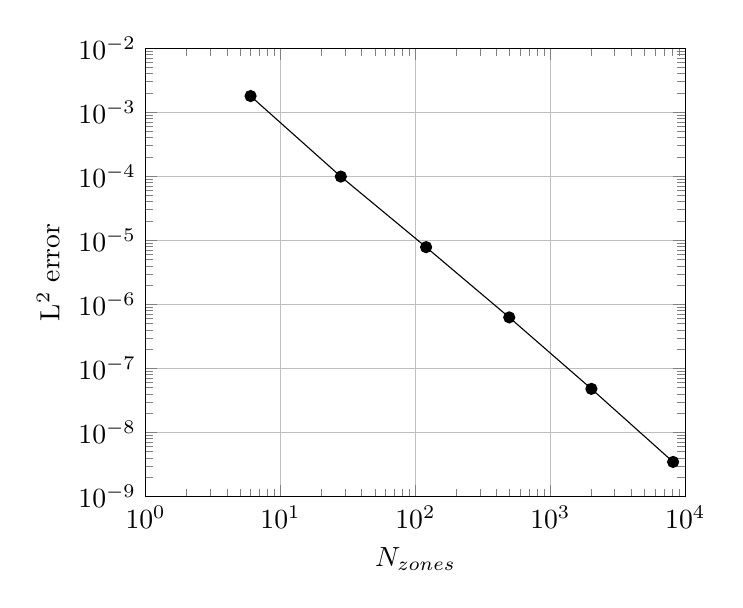
\begin{tikzpicture}
  \begin{axis}[
    %width=0.9\textwidth,
    %height=0.9\textwidth,
    grid=major,
    xlabel={$N_\text{zones}$},
    ylabel={L$^2$ error},
  	xmode=log,
  	ymode=log,
  	xmin=1,xmax=1e4,
  	ymin=1e-9,ymax=1e-2,
  	]
\addplot[mark=*, mark size=2, draw=black, mark options={solid, fill=black}] table[row sep=crcr] {
6 0.0017878942 \\
28 9.8887338e-05 \\
120 7.8171296e-06 \\
496 6.2560514e-07 \\
2016 4.7915253e-08 \\
8128 3.4625793e-09 \\};

  \end{axis}\end{tikzpicture}
\caption{Accuracy of solutions for given mesh refinement for $p=4$ using $S_8$ level-symmetric angular quadrature on a $1^\text{st}$-order mesh.}
\label{fig:RZASMMSLinearRhoBrunnerp4S8g1Accuracy}
\end{figure}


%%%%%%%%%%%%%%%%%%%%%%%%%%%%%%%%%%%%%%%
%%%%%%%%%%%%%%%%%%%%%%%%%%%%%%%%%%%%%%%
%%%%%%%%%%%%%%%%%%%%%%%%%%%%%%%%%%%%%%%
%%%%%%%%%%%%%%%%%%%%%%%%%%%%%%%%%%%%%%%
\FloatBarrier

%%%%%%%%%%%%%%%%%%%%%%%%%%%%%%%%%%%%%%%
\subsubsubsection{High-Order Mesh}
\label{subsec:HOMesh}
Now, we perform the same asymmetry analysis using a high-order mesh. In this section, we observe the sensitivity of the scalar flux spherical asymmetry to changing the discrete ordinates order, finite element order, and spatial refinement on a high-order mesh. A high-order mesh is one that has curved polynomial surfaces. Specifically, we use $2^\text{nd}$-order meshes here. The vertices of the $2^\text{nd}$-order meshes used in this section are located in concentric rings of equal $\rho=\sqrt{r^2+z^2}$, including the midpoint vertices. The results in this section are organized as follows: comparing the discrete ordinates order for each of $p=\{1,2,4\}$, comparing each of $p=\{1,2,4\}$ for $S_8$ level symmetric angular quadrature, mesh refinement studies for each of $p=\{1,4\}$, and comparing the discrete ordinates refinement on the most refined spatial mesh.

Figure~\ref{fig:RZASMMSLinearRhoBrunnerp1g2r2} shows the $\phi_\text{asym}$ values calculated using Equation~\ref{eq:RelativeAsymmetry} for $1^\text{st}$-order finite elements on a $2^\text{nd}$-order mesh with 120 zones for several angular quadrature discretizations. The asymmetry is plotted on a log scale. The scale colors assist in demonstrating the qualitative locations of the asymmetries. The yellow region is the least symmetric, red regions have increased symmetry, and blue regions have the most symmetry. The $\phi_\text{asym}$ solution is plotted using the same finite element shape functions as the scalar flux. There is no perceptible gain in symmetry by increasing the angular discretization order. We confirm this by plotting the asymmetry values as a function of the spherical radius (i.e., $\rho=\sqrt{r^2+z^2}$) in Figure~\ref{fig:RZASMMSLinearRhoBrunnerp1g2r2Nodes}. The spherical radial asymmetry solutions are indistinguishable between discrete ordinate orders. Moreover, Figure~\ref{fig:RZASMMSLinearRhoBrunnerp1g2r2Accuracy} demonstrates there is no increase in accuracy by increasing the $S_N$ order.

\begin{sidewaysfigure}[!htb]
\centering
\begin{subfigure}{0.33\textwidth}
\includegraphics[scale=0.3,trim={50pt 70pt 320pt 45pt},clip]{../../Research/graphics/Axisymmetry/RZASMMSLinearRhoBrunner/p1S4g2r2}
\caption{$S_4$.}
\end{subfigure}%
%\begin{subfigure}{0.2\textwidth}
%\includegraphics[scale=0.25,trim={50pt 70pt 320pt 45pt},clip]{../../Research/graphics/Axisymmetry/RZASMMSLinearRhoBrunner/p1S6g2r2}
%\caption{$S_6$.}
%\end{subfigure}%
\begin{subfigure}{0.33\textwidth}
\includegraphics[scale=0.3,trim={50pt 70pt 320pt 45pt},clip]{../../Research/graphics/Axisymmetry/RZASMMSLinearRhoBrunner/p1S8g2r2}
\caption{$S_8$.}
\end{subfigure}%
%\begin{subfigure}{0.2\textwidth}
%\includegraphics[scale=0.25,trim={50pt 70pt 320pt 45pt},clip]{../../Research/graphics/Axisymmetry/RZASMMSLinearRhoBrunner/p1S10g2r2}
%\caption{$S_{10}$.}
%\end{subfigure}%
\begin{subfigure}{0.33\textwidth}
\includegraphics[scale=0.3,trim={50pt 70pt 320pt 45pt},clip]{../../Research/graphics/Axisymmetry/RZASMMSLinearRhoBrunner/p1S12g2r2}
\caption{$S_{12}$.}
\end{subfigure}
\caption{Relative asymmetry for $1^\text{st}$-order finite elements on a $2^\text{nd}$-order mesh for given order of level-symmetric angular quadrature.}
\label{fig:RZASMMSLinearRhoBrunnerp1g2r2}
\end{sidewaysfigure}

\begin{figure}[!htb]
\centering
\includegraphics[scale=1]{./graphics/RZASMMSLinearRhoBrunnerp1g2r2.pdf}
\caption{Measure of the asymmetry for each finite element node for the given level-symmetric angular quadrature order for $1^\text{st}$-order DFEM and $2^\text{nd}$-order mesh with 120 zones (see Figure~\ref{fig:RZASMMSLinearRhoBrunnerp1g2r2}).}
\label{fig:RZASMMSLinearRhoBrunnerp1g2r2Nodes}
\end{figure}

\begin{figure}[!htb]
\centering
\begin{tikzpicture}
  \begin{axis}[
    %width=0.9\textwidth,
    %height=0.9\textwidth,
    grid=major,
    xlabel={$S_N$},
    ylabel={L$^2$ error},
  	%xmode=log,
  	ymode=log,
  	xmin=4,xmax=12,
  	ymin=1e-4,ymax=1e-3,
  	]
\addplot[mark=*, mark size=2, draw=black, mark options={solid, fill=black}] table[row sep=crcr] {
4 0.00064411998 \\
6 0.00069161191 \\
8 0.00071301712 \\
10 0.0007189547 \\
12 0.0007243029 \\};

  \end{axis}
\end{tikzpicture}
\caption{Accuracy of solutions for given angular quadrature using $p=1$ on a $2^\text{nd}$-order mesh with 120 zones.}
\label{fig:RZASMMSLinearRhoBrunnerp1g2r2Accuracy}
\end{figure}

\FloatBarrier

Figure~\ref{fig:RZASMMSLinearRhoBrunnerp2g2r2} shows the $\phi_\text{asym}$ values calculated using Equation~\ref{eq:RelativeAsymmetry} for $2^\text{nd}$-order finite elements on a $2^\text{nd}$-order mesh with 120 zones for several angular quadrature discretizations. The asymmetry is plotted on a log scale. The scale colors assist in demonstrating the qualitative locations of the asymmetries. The yellow region is the least symmetric, red regions have increased symmetry, and blue regions have the most symmetry. The $\phi_\text{asym}$ solution is plotted using the same finite element shape functions as the scalar flux. There is very little perceptible gain in symmetry near the equator (i.e., $z=0$) by increasing the angular discretization order. However, plotting the asymmetry values as a function of the spherical radius (i.e., $\rho=\sqrt{r^2+z^2}$) in Figure~\ref{fig:RZASMMSLinearRhoBrunnerp2g2r2Nodes} shows that there may not actually be any symmetry gains --- the spherical radial asymmetry solutions are indistinguishable between discrete ordinate orders. The asymmetries are predominantly located near the polar axis (i.e., $r=0$). Moreover, Figure~\ref{fig:RZASMMSLinearRhoBrunnerp2g2r2Accuracy} demonstrates there is no increase in accuracy by increasing the $S_N$ order.

\begin{sidewaysfigure}[!htb]
\centering
\begin{subfigure}{0.33\textwidth}
\includegraphics[scale=0.3,trim={50pt 70pt 320pt 45pt},clip]{../../Research/graphics/Axisymmetry/RZASMMSLinearRhoBrunner/p2S4g2r2}
\caption{$S_4$.}
\end{subfigure}%
%\begin{subfigure}{0.2\textwidth}
%\includegraphics[scale=0.25,trim={50pt 70pt 320pt 45pt},clip]{../../Research/graphics/Axisymmetry/RZASMMSLinearRhoBrunner/p2S6g2r2}
%\caption{$S_6$.}
%\end{subfigure}%
\begin{subfigure}{0.33\textwidth}
\includegraphics[scale=0.3,trim={50pt 70pt 320pt 45pt},clip]{../../Research/graphics/Axisymmetry/RZASMMSLinearRhoBrunner/p2S8g2r2}
\caption{$S_8$.}
\end{subfigure}%
%\begin{subfigure}{0.2\textwidth}
%\includegraphics[scale=0.25,trim={50pt 70pt 320pt 45pt},clip]{../../Research/graphics/Axisymmetry/RZASMMSLinearRhoBrunner/p2S10g2r2}
%\caption{$S_{10}$.}
%\end{subfigure}%
\begin{subfigure}{0.33\textwidth}
\includegraphics[scale=0.3,trim={50pt 70pt 320pt 45pt},clip]{../../Research/graphics/Axisymmetry/RZASMMSLinearRhoBrunner/p2S12g2r2}
\caption{$S_{12}$.}
\end{subfigure}
\caption{Relative asymmetry for $2^\text{nd}$-order finite elements on a $2^\text{nd}$-order mesh for given order of level-symmetric angular quadrature.}
\label{fig:RZASMMSLinearRhoBrunnerp2g2r2}
\end{sidewaysfigure}

\begin{figure}[!htb]
\centering
\includegraphics[scale=1]{./graphics/RZASMMSLinearRhoBrunnerp2g2r2.pdf}
\caption{Measure of the asymmetry for each finite element node for the given level-symmetric angular quadrature order for $2^\text{nd}$-order DFEM and $2^\text{nd}$-order mesh with 120 zones (see Figure~\ref{fig:RZASMMSLinearRhoBrunnerp2g2r2}).}
\label{fig:RZASMMSLinearRhoBrunnerp2g2r2Nodes}
\end{figure}

\begin{figure}[!htb]
\centering
\begin{tikzpicture}
  \begin{axis}[
    %width=0.9\textwidth,
    %height=0.9\textwidth,
    grid=major,
    xlabel={$S_N$},
    ylabel={L$^2$ error},
  	%xmode=log,
  	ymode=log,
  	xmin=4,xmax=12,
  	ymin=1e-5,ymax=1e-4,
  	]
\addplot[mark=*, mark size=2, draw=black, mark options={solid, fill=black}] table[row sep=crcr] {
4 3.8385033e-05 \\
6 4.0476249e-05 \\
8 4.1717384e-05 \\
10 4.188467e-05 \\
12 4.2002395e-05 \\};

  \end{axis}
\end{tikzpicture}
\caption{Accuracy of solutions for given angular quadrature using $p=2$ on a $2^\text{nd}$-order mesh with 120 zones.}
\label{fig:RZASMMSLinearRhoBrunnerp2g2r2Accuracy}
\end{figure}

\FloatBarrier

Figure~\ref{fig:RZASMMSLinearRhoBrunnerp4g2r2} shows the $\phi_\text{asym}$ values calculated using Equation~\ref{eq:RelativeAsymmetry} for $4^\text{th}$-order finite elements on a $2^\text{nd}$-order mesh with 120 zones for several angular quadrature discretizations. The asymmetry is plotted on a log scale. The scale colors assist in demonstrating the qualitative locations of the asymmetries. The yellow region is the least symmetric, red regions have increased symmetry, and blue regions have the most symmetry. The $\phi_\text{asym}$ solution is plotted using the same finite element shape functions as the scalar flux. There is no perceptible gain in symmetry by increasing the angular discretization order. However, plotting the asymmetry values as a function of the spherical radius (i.e., $\rho=\sqrt{r^2+z^2}$) in Figure~\ref{fig:RZASMMSLinearRhoBrunnerp4g2r2Nodes} shows that there may be a symmetry gain from $S_4$ to higher angular discretization orders for $\rho \geq 0.7$. Unlike Figure~\ref{fig:RZASMMSLinearRhoBrunnerp2g2r2}, the asymmetry of the scalar flux appears to be a function of the spherical radius, $\rho$. Moreover, Figure~\ref{fig:RZASMMSLinearRhoBrunnerp4g2r2Accuracy} demonstrates there is no increase in accuracy by increasing the $S_N$ order.

\begin{sidewaysfigure}[!htb]
\centering
\begin{subfigure}{0.33\textwidth}
\includegraphics[scale=0.3,trim={50pt 70pt 320pt 45pt},clip]{../../Research/graphics/Axisymmetry/RZASMMSLinearRhoBrunner/p4S4g2r2}
\caption{$S_4$.}
\end{subfigure}%
%\begin{subfigure}{0.2\textwidth}
%\includegraphics[scale=0.25,trim={50pt 70pt 320pt 45pt},clip]{../../Research/graphics/Axisymmetry/RZASMMSLinearRhoBrunner/p4S6g2r2}
%\caption{$S_6$.}
%\end{subfigure}%
\begin{subfigure}{0.33\textwidth}
\includegraphics[scale=0.3,trim={50pt 70pt 320pt 45pt},clip]{../../Research/graphics/Axisymmetry/RZASMMSLinearRhoBrunner/p4S8g2r2}
\caption{$S_8$.}
\end{subfigure}%
%\begin{subfigure}{0.2\textwidth}
%\includegraphics[scale=0.25,trim={50pt 70pt 320pt 45pt},clip]{../../Research/graphics/Axisymmetry/RZASMMSLinearRhoBrunner/p4S10g2r2}
%\caption{$S_{10}$.}
%\end{subfigure}%
\begin{subfigure}{0.33\textwidth}
\includegraphics[scale=0.3,trim={50pt 70pt 320pt 45pt},clip]{../../Research/graphics/Axisymmetry/RZASMMSLinearRhoBrunner/p4S12g2r2}
\caption{$S_{12}$.}
\end{subfigure}
\caption{Relative asymmetry for $4^\text{th}$-order finite elements on a $2^\text{nd}$-order mesh for given order of level-symmetric angular quadrature.}
\label{fig:RZASMMSLinearRhoBrunnerp4g2r2}
\end{sidewaysfigure}

\begin{figure}[!htb]
\centering
\includegraphics[scale=1]{./graphics/RZASMMSLinearRhoBrunnerp4g2r2.pdf}
\caption{Measure of the asymmetry for each finite element node for the given level-symmetric angular quadrature order for $4^\text{th}$-order DFEM and $2^\text{nd}$-order mesh with 120 zones (see Figure~\ref{fig:RZASMMSLinearRhoBrunnerp4g2r2}).}
\label{fig:RZASMMSLinearRhoBrunnerp4g2r2Nodes}
\end{figure}

\begin{figure}[!htb]
\centering
\begin{tikzpicture}
  \begin{axis}[
    %width=0.9\textwidth,
    %height=0.9\textwidth,
    grid=major,
    xlabel={$S_N$},
    ylabel={L$^2$ error},
  	%xmode=log,
  	ymode=log,
  	xmin=4,xmax=12,
  	ymin=1e-6,ymax=1e-5,
  	]
\addplot[mark=*, mark size=2, draw=black, mark options={solid, fill=black}] table[row sep=crcr] {
4 7.0024448e-06 \\
6 7.1721299e-06 \\
8 7.2301065e-06 \\
10 7.2031758e-06 \\
12 7.174231e-06 \\};

  \end{axis}
\end{tikzpicture}
\caption{Accuracy of solutions for given angular quadrature using $p=4$ on a $2^\text{nd}$-order mesh with 120 zones.}
\label{fig:RZASMMSLinearRhoBrunnerp4g2r2Accuracy}
\end{figure}

\FloatBarrier

Figure~\ref{fig:RZASMMSLinearRhoBrunnerS8g2r2CompareP} shows the $\phi_\text{asym}$ values calculated using Equation~\ref{eq:RelativeAsymmetry} for $p=\{1,2,4\}$ finite elements on a $2^\text{nd}$-order mesh with 120 zones with $S_8$ level-symmetric angular quadrature repeated from Figures~\ref{fig:RZASMMSLinearRhoBrunnerp1g2r2},~\ref{fig:RZASMMSLinearRhoBrunnerp2g2r2},~\ref{fig:RZASMMSLinearRhoBrunnerp4g2r2} and plotted on the same scale. Increasing the finite element order from $p=1$ to $p=2$ increases the symmetry near the origin slightly, indicated by a reduction in yellow. However, increasing the finite element order to $p=4$ provides significant gains in symmetry shown by the relatively larger blue region for $\rho=\sqrt{r^2+z^2} \geq 0.5$. We corroborate these results by plotting the asymmetry values as a function of the spherical radius (i.e., $\rho=\sqrt{r^2+z^2}$) in Figure~\ref{fig:RZASMMSLinearRhoBrunnerS8g2r2Nodes}. It is evident that increasing the finite element order provides gains in spherical symmetry. Moreover, Figure~\ref{fig:RZASMMSLinearRhoBrunnerS8g2r2Accuracy} demonstrates there is an increase in accuracy by increasing the finite element order.

\begin{sidewaysfigure}[!htb]
\centering
\begin{subfigure}{0.33\textwidth}
\includegraphics[scale=0.3,trim={50pt 70pt 320pt 45pt},clip]{../../Research/graphics/Axisymmetry/RZASMMSLinearRhoBrunner/p1S8g2r2CompP}
\caption{$p=1$.}
\end{subfigure}%
\begin{subfigure}{0.33\textwidth}
\includegraphics[scale=0.3,trim={50pt 70pt 320pt 45pt},clip]{../../Research/graphics/Axisymmetry/RZASMMSLinearRhoBrunner/p2S8g2r2CompP}
\caption{$p=2$.}
\end{subfigure}%
\begin{subfigure}{0.33\textwidth}
\includegraphics[scale=0.3,trim={50pt 70pt 320pt 45pt},clip]{../../Research/graphics/Axisymmetry/RZASMMSLinearRhoBrunner/p4S8g2r2CompP}
\caption{$p=4$.}
\end{subfigure}
\caption{Relative asymmetry for $p=\{1,2,4\}$ finite elements on a $2^\text{nd}$-order mesh for $S_8$ level-symmetric angular quadrature.}
\label{fig:RZASMMSLinearRhoBrunnerS8g2r2CompareP}
\end{sidewaysfigure}

\begin{figure}[!htb]
\centering
\includegraphics[scale=1]{./graphics/RZASMMSLinearRhoBrunnerS8g2r2.pdf}
\caption{Measure of the asymmetry for each finite element node for the given finite element order using $S_8$ level-symmetric angular quadrature on a $2^\text{nd}$-order mesh with 120 zones (see Figure~\ref{fig:RZASMMSLinearRhoBrunnerS8g2r2CompareP}).}
\label{fig:RZASMMSLinearRhoBrunnerS8g2r2Nodes}
\end{figure}

\begin{figure}[!htb]
\centering
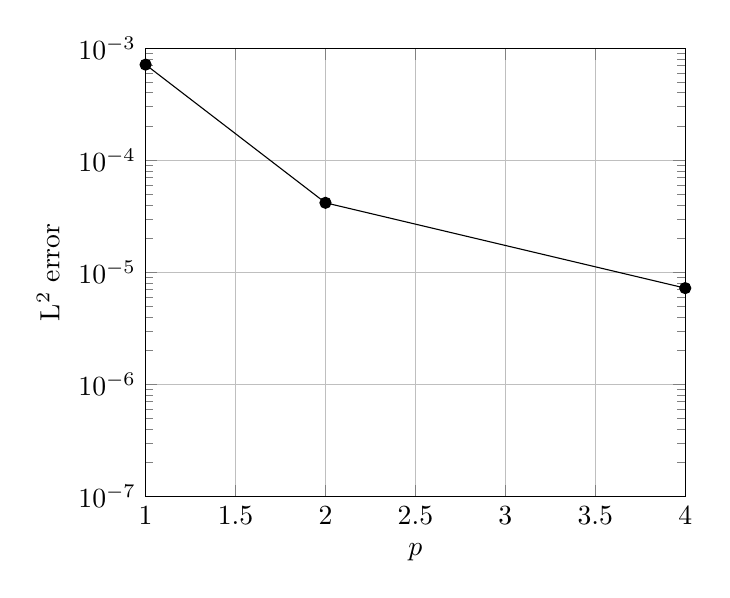
\begin{tikzpicture}
  \begin{axis}[
    %width=0.9\textwidth,
    %height=0.9\textwidth,
    grid=major,
    xlabel={$p$},
    ylabel={L$^2$ error},
  	%xmode=log,
  	ymode=log,
  	xmin=1,xmax=4,
  	ymin=1e-7,ymax=1e-3,
  	]
\addplot[mark=*, mark size=2, draw=black, mark options={solid, fill=black}] table[row sep=crcr] {
1 0.00071301712 \\
2 4.1717384e-05 \\
4 7.2301065e-06 \\};

  \end{axis}
\end{tikzpicture}
\caption{Accuracy of solutions for given angular quadrature using $S_8$ level-symmetric angular quadrature on a $2^\text{nd}$-order mesh with 120 zones.}
\label{fig:RZASMMSLinearRhoBrunnerS8g2r2Accuracy}
\end{figure}

\FloatBarrier

We investigated the symmetry preservation by performing sequential mesh refinements for $p=1$ with $S_8$ level-symmetric angular quadrature. Figures~\ref{fig:RZASMMSLinearRhoBrunnerp1S8g2Part1}~and~\ref{fig:RZASMMSLinearRhoBrunnerp1S8g2Part2} show the first several mesh refinement steps. The asymmetry is plotted on a log scale. The scale colors assist in demonstrating the qualitative locations of the asymmetries. The yellow region is the least symmetric, red regions have increased symmetry, and blue regions have the most symmetry. The $\phi_\text{asym}$ solution is plotted using the same finite element shape functions as the scalar flux. As on the $1^\text{st}$-order mesh, there is tremendous gain (many orders of magnitude) in symmetry by refining the $2^\text{nd}$-order mesh. We observe large regions of $\phi_\text{asym}$ changing from yellow to red to blue throughout the mesh refinement. Plotting the symmetry values as a function of the spherical radius (i.e., $\rho=\sqrt{r^2+z^2}$) in Figure~\ref{fig:RZASMMSLinearRhoBrunnerp1S8g2Nodes} confirms the substantial symmetry gain by refining the mesh. The largest asymmetry magnitude of the scalar flux remains near the origin (i.e. $\rho=\sqrt{r^2+z^2}=0$) as previously seen, but also remains prevalent in the discrete ordinates directions as though there were ray effects. Moreover, Figure~\ref{fig:RZASMMSLinearRhoBrunnerp1S8g2Accuracy} demonstrates there is an increase in accuracy by refining the spatial mesh.

\begin{sidewaysfigure}[!htb]
\centering
\begin{subfigure}{0.33\textwidth}
\includegraphics[scale=0.3,trim={50pt 70pt 320pt 45pt},clip]{../../Research/graphics/Axisymmetry/RZASMMSLinearRhoBrunner/p1S8g2r0CompR}
\caption{$N_\text{zones}=6$.}
\end{subfigure}%
\begin{subfigure}{0.33\textwidth}
\includegraphics[scale=0.3,trim={50pt 70pt 320pt 45pt},clip]{../../Research/graphics/Axisymmetry/RZASMMSLinearRhoBrunner/p1S8g2r1CompR}
\caption{$N_\text{zones}=28$.}
\end{subfigure}%
\begin{subfigure}{0.33\textwidth}
\includegraphics[scale=0.3,trim={50pt 70pt 320pt 45pt},clip]{../../Research/graphics/Axisymmetry/RZASMMSLinearRhoBrunner/p1S8g2r2CompR}
\caption{$N_\text{zones}=120$.}
\end{subfigure}
\caption{Relative asymmetry for $p=1$ finite elements on a $2^\text{nd}$-order mesh for $S_8$ level-symmetric angular quadrature.}
\label{fig:RZASMMSLinearRhoBrunnerp1S8g2Part1}
\end{sidewaysfigure}

\begin{sidewaysfigure}[!htb]
\centering
\begin{subfigure}{0.33\textwidth}
\includegraphics[scale=0.3,trim={50pt 70pt 320pt 45pt},clip]{../../Research/graphics/Axisymmetry/RZASMMSLinearRhoBrunner/p1S8g2r3CompR}
\caption{$N_\text{zones}=496$.}
\end{subfigure}%
\begin{subfigure}{0.33\textwidth}
\includegraphics[scale=0.3,trim={50pt 70pt 320pt 45pt},clip]{../../Research/graphics/Axisymmetry/RZASMMSLinearRhoBrunner/p1S8g2r4CompR}
\caption{$N_\text{zones}=2016$.}
\end{subfigure}%
\begin{subfigure}{0.33\textwidth}
\includegraphics[scale=0.3,trim={50pt 70pt 320pt 45pt},clip]{../../Research/graphics/Axisymmetry/RZASMMSLinearRhoBrunner/p1S8g2r5CompR}
\caption{$N_\text{zones}=8128$.}
\end{subfigure}
\caption{Relative asymmetry for $p=1$ finite elements on a $2^\text{nd}$-order mesh for $S_8$ level-symmetric angular quadrature; mesh overlay may be removed for clarity.}
\label{fig:RZASMMSLinearRhoBrunnerp1S8g2Part2}
\end{sidewaysfigure}

\begin{figure}[!htb]
\centering
\includegraphics[scale=1]{./graphics/RZASMMSLinearRhoBrunnerp1S8g2}
\caption{Measure of the asymmetry for each finite element node for $1^\text{st}$-order finite elements using $S_8$ level-symmetric angular quadrature on a $2^\text{nd}$-order mesh with various number of zones (see Figures~\ref{fig:RZASMMSLinearRhoBrunnerp1S8g2Part1}-\ref{fig:RZASMMSLinearRhoBrunnerp1S8g2Part2}).}
\label{fig:RZASMMSLinearRhoBrunnerp1S8g2Nodes}
\end{figure}

\begin{figure}[!htb]
\centering
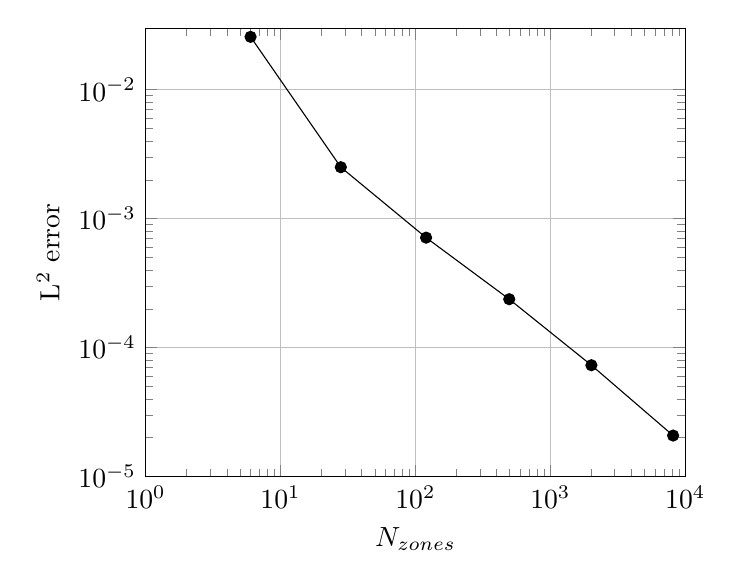
\begin{tikzpicture}
  \begin{axis}[
    %width=0.9\textwidth,
    %height=0.9\textwidth,
    grid=major,
    xlabel={$N_\text{zones}$},
    ylabel={L$^2$ error},
  	xmode=log,
  	ymode=log,
  	xmin=1,xmax=1e4,
  	ymin=1e-5,ymax=3e-2,
  	]
\addplot[mark=*, mark size=2, draw=black, mark options={solid, fill=black}] table[row sep=crcr] {
6 0.025725225 \\
28 0.0025077394 \\
120 0.00071301712 \\
496 0.00023746835 \\
2016 7.3058318e-05 \\
8128 2.080903e-05 \\};

  \end{axis}
\end{tikzpicture}
\caption{Accuracy of solutions for mesh refinement study using $p=1$, $S_8$ level-symmetric angular quadrature, on a $2^\text{nd}$-order mesh.}
\label{fig:RZASMMSLinearRhoBrunnerp1S8g2Accuracy}
\end{figure}

\FloatBarrier

We also investigated the symmetry preservation by performing sequential mesh refinements for $p=1$ with $S_8$ level-symmetric angular quadrature. Figures~\ref{fig:RZASMMSLinearRhoBrunnerp4S8g2Part1}~and~\ref{fig:RZASMMSLinearRhoBrunnerp4S8g2Part2} show the first several mesh refinement steps. The asymmetry is plotted on a log scale. The scale colors assist in demonstrating the qualitative locations of the asymmetries. The yellow region is the least symmetric, red regions have increased symmetry, and blue regions have the most symmetry. The $\phi_\text{asym}$ solution is plotted using the same finite element shape functions as the scalar flux. As on the $1^\text{st}$-order mesh, there is tremendous gain (many orders of magnitude) in symmetry by refining the $2^\text{nd}$-order mesh. We observe large regions of $\phi_\text{asym}$ changing from yellow to red to blue throughout the mesh refinement. Plotting the symmetry values as a function of the spherical radius (i.e., $\rho=\sqrt{r^2+z^2}$) in Figure~\ref{fig:RZASMMSLinearRhoBrunnerp4S8g2Nodes} confirms the substantial symmetry gain by refining the mesh. The largest asymmetry magnitude of the scalar flux remains near the origin (i.e. $\rho=\sqrt{r^2+z^2}=0$) as previously seen, but also remains prevalent in the discrete ordinates directions as though there were ray effects. Moreover, Figure~\ref{fig:RZASMMSLinearRhoBrunnerp4S8g2Accuracy} demonstrates there is an increase in accuracy by refining the spatial mesh.

\begin{sidewaysfigure}[!htb]
\centering
\begin{subfigure}{0.33\textwidth}
\includegraphics[scale=0.3,trim={50pt 70pt 320pt 45pt},clip]{../../Research/graphics/Axisymmetry/RZASMMSLinearRhoBrunner/p4S8g2r0CompR}
\caption{$N_\text{zones}=6$.}
\end{subfigure}%
\begin{subfigure}{0.33\textwidth}
\includegraphics[scale=0.3,trim={50pt 70pt 320pt 45pt},clip]{../../Research/graphics/Axisymmetry/RZASMMSLinearRhoBrunner/p4S8g2r1CompR}
\caption{$N_\text{zones}=28$.}
\end{subfigure}%
\begin{subfigure}{0.33\textwidth}
\includegraphics[scale=0.3,trim={50pt 70pt 320pt 45pt},clip]{../../Research/graphics/Axisymmetry/RZASMMSLinearRhoBrunner/p4S8g2r2CompR}
\caption{$N_\text{zones}=120$.}
\end{subfigure}
\caption{Relative asymmetry for $p=4$ finite elements on a $2^\text{nd}$-order mesh for $S_8$ level-symmetric angular quadrature.}
\label{fig:RZASMMSLinearRhoBrunnerp4S8g2Part1}
\end{sidewaysfigure}

\begin{sidewaysfigure}[!htb]
\centering
\begin{subfigure}{0.33\textwidth}
\includegraphics[scale=0.3,trim={50pt 70pt 320pt 45pt},clip]{../../Research/graphics/Axisymmetry/RZASMMSLinearRhoBrunner/p4S8g2r3CompR}
\caption{$N_\text{zones}=496$.}
\end{subfigure}%
\begin{subfigure}{0.33\textwidth}
\includegraphics[scale=0.3,trim={50pt 70pt 320pt 45pt},clip]{../../Research/graphics/Axisymmetry/RZASMMSLinearRhoBrunner/p4S8g2r4CompR}
\caption{$N_\text{zones}=2016$.}
\end{subfigure}%
\begin{subfigure}{0.33\textwidth}
\includegraphics[scale=0.3,trim={50pt 70pt 320pt 45pt},clip]{../../Research/graphics/Axisymmetry/RZASMMSLinearRhoBrunner/p4S8g2r5CompR}
\caption{$N_\text{zones}=8128$.}
\end{subfigure}
\caption{Relative asymmetry for $p=4$ finite elements on a $2^\text{nd}$-order mesh for $S_8$ level-symmetric angular quadrature; mesh overlay may be removed for clarity.}
\label{fig:RZASMMSLinearRhoBrunnerp4S8g2Part2}
\end{sidewaysfigure}

\begin{figure}[!htb]
\centering
\includegraphics[scale=1]{./graphics/RZASMMSLinearRhoBrunnerp4S8g2.pdf}
\caption{Measure of the asymmetry for each finite element node for $4^\text{th}$-order DFEM, $S_8$ level-symmetric angular quadrature, and $2^\text{nd}$-order mesh with various number of zones (see Figures~\ref{fig:RZASMMSLinearRhoBrunnerp4S8g2Part1}~-~\ref{fig:RZASMMSLinearRhoBrunnerp4S8g2Part2}).}
\label{fig:RZASMMSLinearRhoBrunnerp4S8g2Nodes}
\end{figure}

\begin{figure}[!htb]
\centering
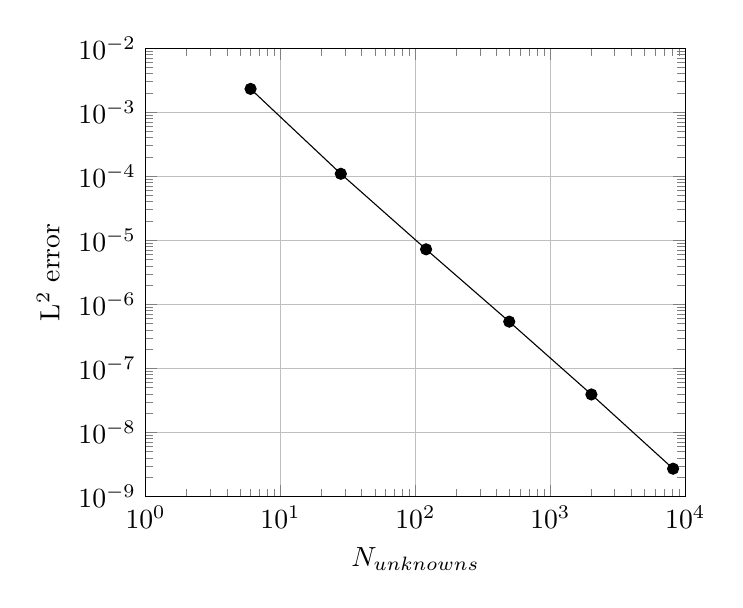
\begin{tikzpicture}
  \begin{axis}[
    %width=0.9\textwidth,
    %height=0.9\textwidth,
    grid=major,
    xlabel={$N_\text{unknowns}$},
    ylabel={L$^2$ error},
  	xmode=log,
  	ymode=log,
  	xmin=1,xmax=1e4,
  	ymin=1e-9,ymax=1e-2,
  	]
\addplot[mark=*, mark size=2, draw=black, mark options={solid, fill=black}] table[row sep=crcr] {
6 0.0023130263 \\
28 0.00010926868 \\
120 7.2301065e-06 \\
496 5.3684571e-07 \\
2016 3.9184195e-08 \\
8128 2.714164e-09 \\};

  \end{axis}
\end{tikzpicture}
\caption{Accuracy of solutions for mesh refinement study using $p=4$, $S_8$ level-symmetric angular quadrature, on a $2^\text{nd}$-order mesh.}
\label{fig:RZASMMSLinearRhoBrunnerp4S8g2Accuracy}
\end{figure}

\FloatBarrier

In the most refined case of Figures~\ref{fig:RZASMMSLinearRhoBrunnerp1S8g2Part2}~and~\ref{fig:RZASMMSLinearRhoBrunnerp4S8g2Part2}, we observe some ray effects. These effects are dependent on the discrete ordinates discretization order. Here, we investigate the symmetry preservation by performing sequential discrete ordinates refinements for $p=1$ on a $2^\text{nd}$-order mesh with 8128 zones. Figure~\ref{fig:RZASMMSLinearRhoBrunnerp1g2r5} show the first several mesh refinement steps. The asymmetry is plotted on a log scale. The scale colors assist in demonstrating the qualitative locations of the asymmetries. The yellow region is the least symmetric, red regions have increased symmetry, and blue regions have the most symmetry. The $\phi_\text{asym}$ solution is plotted using the same finite element shape functions as the scalar flux. The ray effects are dependent upon the discrete ordinates discretization order. Despite the appearance of a reduction in overall symmetry, plotting the symmetry values as a function of the spherical radius (i.e., $\rho=\sqrt{r^2+z^2}$) in Figure~\ref{fig:RZASMMSLinearRhoBrunnerp4S8g2Nodes} demonstrates that the overall asymmetry is not very dependent upon the discrete ordinates discretization. The locations of these ray effects may introduce asymmetries themselves when coupling to other physics.

\begin{sidewaysfigure}[!htb]
\centering
\begin{subfigure}{0.33\textwidth}
\includegraphics[scale=0.3,trim={50pt 70pt 320pt 45pt},clip]{../../Research/graphics/Axisymmetry/RZASMMSLinearRhoBrunner/p1S4g2r5}
\caption{$S_4$.}
\end{subfigure}%
%\begin{subfigure}{0.2\textwidth}
%\includegraphics[scale=0.25,trim={50pt 70pt 320pt 45pt},clip]{../../Research/graphics/Axisymmetry/RZASMMSLinearRhoBrunner/p1S6g2r5}
%\caption{$S_6$.}
%\end{subfigure}%
\begin{subfigure}{0.33\textwidth}
\includegraphics[scale=0.3,trim={50pt 70pt 320pt 45pt},clip]{../../Research/graphics/Axisymmetry/RZASMMSLinearRhoBrunner/p1S8g2r5-2}
\caption{$S_8$ (repeated from Fig.~\ref{fig:RZASMMSLinearRhoBrunnerp1S8g2Part2}).}
\end{subfigure}%
%\begin{subfigure}{0.2\textwidth}
%\includegraphics[scale=0.25,trim={50pt 70pt 320pt 45pt},clip]{../../Research/graphics/Axisymmetry/RZASMMSLinearRhoBrunner/p1S10g2r5}
%\caption{$S_{10}$.}
%\end{subfigure}%
\begin{subfigure}{0.33\textwidth}
\includegraphics[scale=0.3,trim={50pt 70pt 320pt 45pt},clip]{../../Research/graphics/Axisymmetry/RZASMMSLinearRhoBrunner/p1S12g2r5}
\caption{$S_{12}$.}
\end{subfigure}
\caption{Relative asymmetry for $p=1$ finite elements on a $2^\text{nd}$-order mesh with 8128 zones; mesh overlay may be removed for clarity.}
\label{fig:RZASMMSLinearRhoBrunnerp1g2r5}
\end{sidewaysfigure}

We also plot the asymmetry values as a function of the spherical radius (i.e., $\rho=\sqrt{r^2+z^2}$). Figure~\ref{fig:RZASMMSLinearRhoBrunnerp1g2r5Nodes} shows the $\phi_\text{asym}$ values calculated using Equation~\ref{eq:RelativeAsymmetry} for $1^\text{st}$-order finite elements on a $2^\text{nd}$-order mesh with 8128 zones for several angular quadrature discretizations. Moreover, Figure~\ref{fig:RZASMMSLinearRhoBrunnerp4g2r5Accuracy} demonstrates there is no increase in accuracy by increasing the $S_N$ order.

\begin{figure}[!htb]
\centering
\includegraphics[scale=1]{./graphics/RZASMMSLinearRhoBrunnerp1g2r5.pdf}
\caption{Measure of the asymmetry for each finite element node for the given level-symmetric angular quadrature order for $1^\text{st}$-order DFEM and $2^\text{nd}$-order mesh with 8128 zones.}
\label{fig:RZASMMSLinearRhoBrunnerp1g2r5Nodes}
\end{figure}

\begin{figure}[!htb]
\centering
\begin{tikzpicture}
  \begin{axis}[
    %width=0.9\textwidth,
    %height=0.9\textwidth,
    grid=major,
    xlabel={$S_N$},
    ylabel={L$^2$ error},
  	%xmode=log,
  	ymode=log,
  	xmin=4,xmax=12,
  	ymin=1e-5,ymax=1e-4,
  	]
\addplot[mark=*, mark size=2, draw=black, mark options={solid, fill=black}] table[row sep=crcr] {
4 2.1057152e-05 \\
6 2.0826499e-05 \\
8 2.080903e-05 \\
10 2.1015134e-05 \\
12 2.1142207e-05 \\};

  \end{axis}
\end{tikzpicture}
\caption{Accuracy of solutions for given angular quadrature using $p=4$ on a $2^\text{nd}$-order mesh with 8128 zones.}
\label{fig:RZASMMSLinearRhoBrunnerp4g2r5Accuracy}
\end{figure}

\FloatBarrier

%%%%%%%%%%%%%%%%%%%%%%%%%%%%%%%%%%%%%%%
\subsubsubsection{Axisymmety Summary and Discussion}
\label{sub:AxiSymSummaryDiscussion}
For completeness, we compare some of the nodal asymmetry plots for ease of comparing the $2^\text{nd}$-order mesh to the $1^\text{st}$-order mesh on the same scales.

Figure~\ref{fig:RZASMMSLinearRhoBrunnerp1r2NodesSymmetry} compares the $1^\text{st}$-order finite element solutions on both $1^\text{st}$- and $2^\text{nd}$-order meshes.
%
\begin{figure}[!htb]
\centering
\begin{subfigure}{0.48\textwidth}
\centering
\includegraphics[width=\textwidth]{./graphics/RZASMMSLinearRhoBrunnerp1g1r2CompG.pdf}
\caption{$1^\text{st}$-order mesh (adapted from Figure~\ref{fig:RZASMMSLinearRhoBrunnerp1g1r2Nodes}).}
\end{subfigure}%
\hspace{0.04\textwidth}%
\begin{subfigure}{0.48\textwidth}
\centering
\includegraphics[width=\textwidth]{./graphics/RZASMMSLinearRhoBrunnerp1g2r2CompG.pdf}
\caption{$2^\text{nd}$-order mesh (adapted from Figure~\ref{fig:RZASMMSLinearRhoBrunnerp1g2r2Nodes}).}
\end{subfigure}
\caption{Measure of the asymmetry for each finite element node for the given level-symmetric angular quadrature order for $1^\text{st}$-order DFEM on the given mesh with 120 zones.}
\label{fig:RZASMMSLinearRhoBrunnerp1r2NodesSymmetry}
\end{figure}
%
While we have observed that the $S_N$ order does not provide any additional accuracy or spherical symmetry, increasing the mesh order for $1^\text{st}$-order finite elements does increase the spherical symmetry with increasing $\rho$. However, Figure~\ref{fig:RZASMMSLinearRhoBrunnerp4r2NodesSymmetry}
 demonstrates that the mesh curvature does not benefit the spherical symmetry with HO ($4^\text{th}$-order) finite elements.
 %
\begin{figure}[!htb]
\centering
\begin{subfigure}{0.48\textwidth}
\centering
\includegraphics[width=\textwidth]{./graphics/RZASMMSLinearRhoBrunnerp4g1r2CompG.pdf}
\caption{$1^\text{st}$-order mesh (adapted from Figure~\ref{fig:RZASMMSLinearRhoBrunnerp4g1r2Nodes}).}
\end{subfigure}%
\hspace{0.04\textwidth}%
\begin{subfigure}{0.48\textwidth}
\centering
\includegraphics[width=\textwidth]{./graphics/RZASMMSLinearRhoBrunnerp4g2r2CompG.pdf}
\caption{$2^\text{nd}$-order mesh (adapted from Figure~\ref{fig:RZASMMSLinearRhoBrunnerp4g2r2Nodes}).}
\end{subfigure}
\caption{Measure of the asymmetry for each finite element node for the given level-symmetric angular quadrature order for $4^\text{th}$-order DFEM on the given mesh with 120 zones.}
\label{fig:RZASMMSLinearRhoBrunnerp4r2NodesSymmetry}
\end{figure}
%
Finally, Figure~\ref{fig:RZASMMSLinearRhoBrunnerp4S8NodesSymmetry} illustrates that refining the mesh does increase the symmetry preservation for $4^\text{th}$-order finite elements but adding curvature to the mesh zones does not.
%
\begin{figure}[!htb]
\centering
\begin{subfigure}{0.48\textwidth}
\centering
\includegraphics[width=\textwidth]{./graphics/RZASMMSLinearRhoBrunnerp4S8g1CompG.pdf}
\caption{$1^\text{st}$-order mesh (adapted from Figure~\ref{fig:RZASMMSLinearRhoBrunnerp4S8g1Nodes}).}
\end{subfigure}%
\hspace{0.04\textwidth}%
\begin{subfigure}{0.48\textwidth}
\centering
\includegraphics[width=\textwidth]{./graphics/RZASMMSLinearRhoBrunnerp4S8g2CompG.pdf}
\caption{$2^\text{nd}$-order mesh (adapted from Figure~\ref{fig:RZASMMSLinearRhoBrunnerp4S8g2Nodes}).}
\end{subfigure}
\caption{Measure of the asymmetry for each finite element node for $4^\text{th}$-order DFEM, $S_8$ level-symmetric angular quadrature, on the given mesh with various number of zones.}
\label{fig:RZASMMSLinearRhoBrunnerp4S8NodesSymmetry}
\end{figure}

Table~\ref{tab:AxisymmetrySummary} summarizes these findings of whether or not each discretization property reduces the asymmetry or not.
%
\begin{table}[!htb]
\begin{tabular}{|c|c|}
\hline
Property & Reduce Asymmetry? \\\hline
$S_N$ order & no \\\hline
Finite element order & yes \\\hline
mesh refinement & yes \\\hline
mesh curvature & conditional \\\hline
\end{tabular}
\caption{Summary of discretizations and determination of whether they reduce the asymmetry.}
\label{tab:AxisymmetrySummary}
\end{table}

Although the manufactured solution (Eq.~\ref{eq:RZMMSLinearRho}) is seemingly simple, a steep gradient appears in the MMS source term near $(r,z)=(0,0)$. We look at each term of the transport equation using the manufactured solution in Figure~\ref{fig:RZMMSLinearRhoAnalytic}.
%
\begin{figure}[tb]
\includegraphics[scale=0.5]{../../Research/graphics/Axisymmetry/RZASMMSLinearRho/TransportTerms}
\caption{Analytic representation of each term of the transport equation using the manufactured solution, Equation~\ref{eq:RZMMSLinearRho}, for $(\mu,\xi) \approx (0.218,0.951)$. The complicated shapes of the streaming and source terms are typical of the other $\vec{\Omega}$ directions.}
\label{fig:RZMMSLinearRhoAnalytic}
\end{figure}
%
The gradient operated on the manufactured solution generates a very steep gradient near the origin. This contributes to the shape of the source term --- $S_0/(2 \pi)$ is complicated near the origin. In practice, this source is an analytic driver for the radiation field in the problem. The source term is approximated by the finite element shape function using the analytic values for the nodes. So although the source is exact at the node points, the shape function does not capture the analytic shape of the source term necessary to achieve the axisymmetry we desire.


In the future, we will examine this effect of the approximation on the analytical source term by one of two ways. We could utilize the same manufactured solution (Equation~\ref{eq:RZMMSLinearRho}) in a spatial region that does not have as strong of a gradient (i.e., away from the origin). Or, we may have to consider alternative manufactured solutions that avoid the gradient at the origin. It would be ideal to have a manufactured solution that operates well in a region of interest but employing $\rho=\sqrt{r^2+z^2}$ will always result in some form of $\left(r^2+z^2 \right)^{(-1/2)}$ in the streaming term.

\FloatBarrier

%%%%%%%%%%%%%%%%%%%%%%%%%%%%%%%%%%%%%%%
\subsubsection{Strong Scatter with Alternating Boundaries Test}
\label{sec:RZStrongScatter}
We previously tested a higher-order \XY\ transport methodology on an optically thick and highly scattering problem~\cite{WoodsHoDgfemXyCurved}. Here, we perform the same calculation in \RZ\ geometry as originally introduced by Palmer and Adams~\cite{PalmerCurvilinearTransport} and Palmer~
\cite{PalmerDissertation}. The medium is homogeneous, highly scattering ($c=0.999$), has cross sections $\sigma_t=1000 \text{ cm}^{-1}$, $\sigma_s = 999 \text{ cm}^{-1}$, and has no external source. The incident angular flux boundary conditions of strength $\psi_{inc} = 1/(2 \pi) \text{ cm}^{-1} \text{ s}^{-1} \text{ ster}^{-1}$ on alternating locations denoted in Figure~\ref{fig:StrongScatterProblem} by gray bars.
%
\begin{figure}[!htb]
\centering
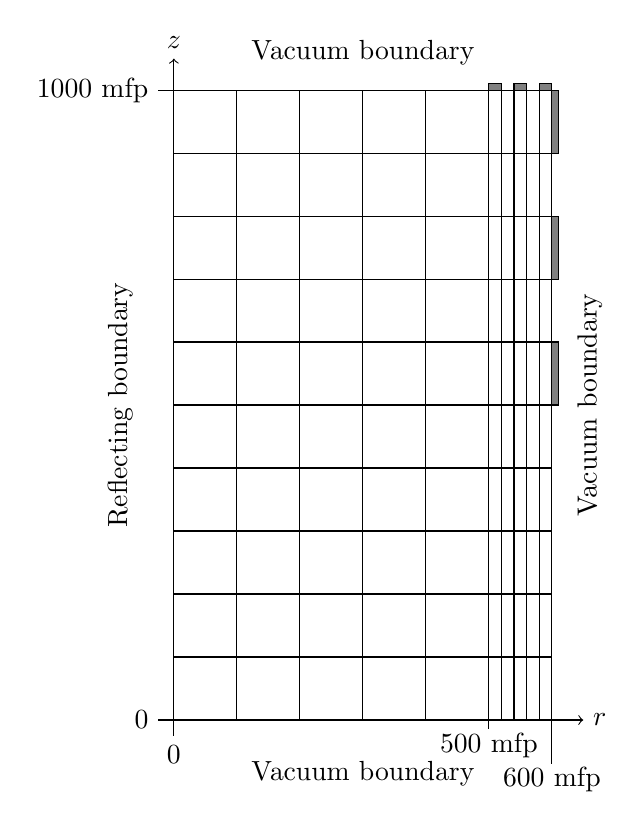
\begin{tikzpicture}[scale=0.8]
\draw [->] (0,0) -- (6.5,0);
\draw [->] (0,0) -- (0,10.5);
\node [above] at (0,10.5) {$z$};
\node [right] at (6.5,0) {$r$};
\draw (0,-0.25) -- (0,0) -- (-0.25,0);
\draw (5,0) -- (5,-0.15);
\draw (6,0) -- (6,-0.7);
\draw (0,10) -- (-0.25,10);
\node [below] at (0,-0.25) {0};
\node [left] at (-0.25,0) {0};
\node [below] at (5,-0.05) {500 mfp};
\node [below] at (6,-0.6) {600 mfp};
\node [left] at (-0.25,10) {1000 mfp};
\node [below] at (3,-0.5) {Vacuum boundary};
\node [above] at (3,10.25) {Vacuum boundary};
\node [right] at (6.25,5) {\rotatebox{90}{Vacuum boundary}};
\node [left] at (-0.5,5) {\rotatebox{90}{Reflecting boundary}};
\draw (5.2,0) -- (5.2,10);
\draw (5.4,0) -- (5.4,10);
\draw (5.6,0) -- (5.6,10);
\draw (5.8,0) -- (5.8,10);
\draw [fill=gray] (5,10) rectangle (5.2,10.1);
\draw [fill=gray] (5.4,10) rectangle (5.6,10.1);
\draw [fill=gray] (5.8,10) rectangle (6,10.1);
\draw [fill=gray] (6,9) rectangle (6.1,10);
\draw [fill=gray] (6,7) rectangle (6.1,8);
\draw [fill=gray] (6,5) rectangle (6.1,6);
\draw (0,0) grid (6,10);
\end{tikzpicture}
\caption{Strong scatter with discontinuous BCs with MIP DSA problem geometry; gray boundaries indicate incident boundary locations.}
\label{fig:StrongScatterProblem}
\end{figure}
%
This incident angular flux strength is an estimated value obtained from other research solving this problem~\cite{PalmerCurvilinearTransport,PalmerDissertation}. For comparison to previous research using BLD, we solve this problem using $p=1$ Gauss-Legendre DGFEM with $S_4$ level-symmetric angular quadrature. The solution is shown in Figure~\ref{fig:RZTP2S4e1}.
%
\begin{figure}[!htb]
\centering
\begin{subfigure}{0.45\textwidth}
\centering
\includegraphics[scale=0.25]{../../Research/graphics/RZTP2S4e1blue}
\captionof{figure}{Scalar flux.}
\label{fig:RZTP2S4e1blue}
\end{subfigure}%
\hspace{0.05\textwidth}
\begin{subfigure}{0.45\textwidth}
\centering
\includegraphics[scale=0.25]{../../Research/graphics/RZTP2S4e1logblue}
\caption{Log of scalar flux.}
\label{fig:RZTP2S4e1logblue}
\end{subfigure}
\caption{Solution to strong scatter with discontinuous boundary conditions with $p=1$ finite elements and $S_4$ level-symmetric angular quadrature. White regions indicate negative scalar fluxes.}
\label{fig:RZTP2S4e1}
\end{figure}
%
While the previous research was investigating lumping techniques to reduce the negative solutions, this work seeks to characterize the behavior of higher-order solutions in \RZ\ geometry. We observe oscillations in the solution that result in some negative scalar fluxes. The solution changes several orders of magnitude. Compared to other research~\cite{PalmerDissertation}, we observe similar oscillations in the boundary layers, however the solution also presents oscillations in the problem interior. This may be due to the use of different basis functions or a result of not discretizing the conservation equation (Eq.~\ref{eq:RZTransport}).

We also solve with $S_8$ level-symmetric angular quadrature using $4^\text{th}$-order finite elements. This solution is shown in Figure~\ref{fig:RZTP2S8e4}.
%
\begin{figure}[!htb]
\centering
\begin{subfigure}{0.45\textwidth}
\centering
\includegraphics[scale=0.25]{../../Research/graphics/RZTP2S8e4blue}
\captionof{figure}{Scalar flux.}
\label{fig:RZTP2S8e4blue}
\end{subfigure}%
\hspace{0.05\textwidth}
\begin{subfigure}{0.45\textwidth}
\centering
\includegraphics[scale=0.25]{../../Research/graphics/RZTP2S8e4logblue}
\caption{Log of scalar flux.}
\label{fig:RZTP2S8e4logblue}
\end{subfigure}
\caption{Solution to strong scatter with discontinuous boundary conditions with $p=4$ finite elements and $S_8$ level-symmetric angular quadrature. White regions indicate negative scalar fluxes.}
\label{fig:RZTP2S8e4}
\end{figure}
%
We observe oscillations in the scalar flux that results in negative solutions. These are predominantly in the boundary layer regions near the upper right and lower left. The solution changes about 20 orders of magnitude.

Comparing Figures~\ref{fig:RZTP2S4e1} and~\ref{fig:RZTP2S8e4}, we observe that the areas of negative solution in the problem interior is suppressed with the use of higher-order finite elements. We also observe that the higher-order FEM modeled a steeper gradient in the solution. The HO solution drove an additional 8 orders of magnitude further than the LO solution. While refining the mesh may help the LO method to model the steep gradient, the HO method was able to do so.

We also solve this problem on a $2^\text{nd}$-order curved mesh. We distort the original mesh by translating the vertices and reconnecting them with $2^\text{nd}$-order polynomials. We solved using $4^\text{th}$-order finite elements and $S_{12}$ level-symmetric angular quadrature. This solution is shown in Figure~\ref{fig:TP2RZS12p4g2}.
%
\begin{figure}[!htb]
\centering
\begin{subfigure}{0.45\textwidth}
\centering
\includegraphics[scale=0.25]{../../Research/graphics/TP2RZS12p4g2blue}
\captionof{figure}{Scalar flux.}
\label{fig:TP2RZS12p4g2blue}
\end{subfigure}%
\hspace{0.05\textwidth}
\begin{subfigure}{0.45\textwidth}
\centering
\includegraphics[scale=0.25]{../../Research/graphics/TP2RZS12p4g2logblue}
\caption{Log of scalar flux.}
\label{fig:TP2RZS12p4g2logblue}
\end{subfigure}
\caption{Solution to strong scatter with discontinuous boundary conditions with $p=4$ finite elements and $S_{12}$ level-symmetric angular quadrature on a $2^\text{nd}$-order mesh. White regions indicate negative scalar fluxes.}
\label{fig:TP2RZS12p4g2}
\end{figure}
%
We observe similar behavior as Figure~\ref{fig:RZTP2S8e4}, indicating that the curved surfaces may not introduce additional errors. Specifically, there are boundary layers that penetrate into the problem interior in the upper-left and bottom-right regions, as well as the slight negativities in the interior near $z=0.5$. From the mesh distortion, some of the zones become larger, resulting in the appearance of larger areas of negative solutions. The reverse is true for zones that became smaller.

\FloatBarrier

%%%%%%%%%%%%%%%%%%%%%%%%%%%%%%%%%%%%%%%
\subsubsection{Material Discontinuity Stress Test}
\label{sec:RZMaterialDiscontinuity}
We adapted this problem from Palmer~\cite{PalmerDissertation} and solved it in \XY\ without DSA in Woods et al.~\cite{WoodsHoDgfemXyCurved}. Presently, we solve this in \RZ\ geometry. There are five different material regions described in Table~\ref{tab:MaterialDiscontinuityProperties} and Figure~\ref{fig:MaterialDiscontinuityMesh}.

\begin{table}[!htb]
\centering
{\renewcommand{\arraystretch}{1.5}
\begin{tabular}{|c|c|c|c|}
\hline
Material Region & $\sigma_t$ cm$^{-1}$ & $\sigma_s$ cm$^{-1}$ & $S_0 \text{ cm}^{-2} \text{ s}^{-1}$ \\\hline
Source & 1.0 & 1.0 & 1.0 \\
Very thin absorber & 0.0001 & 0.0 & 0.0 \\
Thick absorber & 10.0 & 0.0 & 0.0 \\
Very thick absorber & 100.0 & 0.0 & 0.0 \\
Very thick scatterer & 1000.0 & 1000.0 & 0.0 \\
\hline
\end{tabular}}
\caption{Material discontinuity stress test with MIP DSA material properties.}
\label{tab:MaterialDiscontinuityProperties}
\end{table}

\begin{figure}[!hp]
\centering
\begin{tikzpicture}[scale=1]
\node [below] at (0,-0.25) {0};
\node [left] at (-0.25,0) {0};
\node [left] at (-0.25,10) {$z = 1$ cm};
\node [below] at (10,-0.25) {$r = 1$ cm};
\node [below] at (5,-0.5) {Vacuum boundary};
\node [above] at (5,10.25) {Vacuum boundary};
\node [right] at (10.25,5) {\rotatebox{90}{Vacuum boundary}};
\node [left] at (-0.5,5) {\rotatebox{90}{Reflecting boundary}};
\draw [fill=gray] (0,0) rectangle (2,10);
\draw [pattern= north west lines] (2,0) rectangle (6,2);
\draw [pattern=crosshatch dots] (2,2) rectangle (4,10);
\draw [pattern=crosshatch] (6,0) rectangle (10,2);
\draw (0,0) grid (10,10);
\node [fill=white] at (1,5) {Source};
\node [align=center,fill=white] at (4,1) {Very thin\\absorber};
\node [align=center,fill=white] at (3,6) {Thick\\absorber};
\node [align=center,fill=white] at (8,1) {Very thick\\absorber};
\node [align=center,fill=white] at (7,6) {Very thick\\scatterer};
\end{tikzpicture}
\caption{Material discontinuity stress test with MIP DSA problem geometry; materials defined in Table~\ref{tab:MaterialDiscontinuityProperties}.}
\label{fig:MaterialDiscontinuityMesh}
\end{figure}

This problem has cross sections that range several orders of magnitude, resulting in strong material discontinuities. We also introduce anisotropic incident angular fluxes into the scattering region by preferentially attenuating angular fluxes that are not perpendicular to the thick absorber. We expect some degradation in the DSA in problems with strong material discontinuities~\cite{WangDissertation}. We also expect boundary layers to form from the anisotropic incident angular fluxes~\cite{AdamsDFEMDiffLimit}. We solve this using $2^\text{nd}$-order finite elements, $S_4$ level-symmetric angular quadrature, and unaccelerated SI. The scalar flux solution is shown in Figure~\ref{fig:TP2RZS4e2} and the log of the scalar flux is shown in Figure~\ref{fig:TP2RZS4e2log}.
%
\begin{figure}[!htb]
\centering
\begin{subfigure}{\textwidth}
\centering
\includegraphics[scale=0.35,trim={50pt 140pt 50pt 45pt},clip]{../../Research/graphics/TP3RZS4e2}
\captionof{figure}{Scalar flux.}
\label{fig:TP2RZS4e2}
\end{subfigure}
\begin{subfigure}{\textwidth}
\centering
\includegraphics[scale=0.35,trim={50pt 140pt 50pt 45pt},clip]{../../Research/graphics/TP3RZS4e2log}
\caption{Log of scalar flux.}
\label{fig:TP2RZS4e2log}
\end{subfigure}
\caption{Solution to multi-material stress test. White regions indicate negative scalar fluxes.}
\label{fig:RZMultiMaterial}
\end{figure}
%
The white regions are negative fluxes that were removed. We observe a relatively smooth solution throughout most of the problem. There are oscillations (and negativities) in the ``Very thick absorber'' region where the problem is very optically thick. There are very slight numerical artifacts inside the scattering region near the boundary of the ``Very thin absorber'' region.


\FloatBarrier

%%%%%%%%%%%%%%%%%%%%%%%%%%%%%%%%%%%%%%%
%%%%%%%%%%%%%%%%%%%%%%%%%%%%%%%%%%%%%%%
%%%%%%%%%%%%%%%%%%%%%%%%%%%%%%%%%%%%%%%
%%%%%%%%%%%%%%%%%%%%%%%%%%%%%%%%%%%%%%%
%%%%%%%%%%%%%%%%%%%%%%%%%%%%%%%%%%%%%%%
\subsection{Modified Interior Penalty Diffusion Synthetic Acceleration}
\label{sec:ResultsMIP}
In this section, we perform studies of the methodology presented above. This section is divided into two parts: in Section~\ref{sec:MIPDSADirichlet}, we discuss results using the MIP DSA equations with homogeneous Dirichlet boundary conditions, and, in Section~\ref{sec:MIPDSARobin}, we discuss results using the MIP DSA equations with homogeneous Robin boundary conditions. With each of these sections, we perform sensitivity analyses of the spectral radius.

%%%%%%%%%%%%%%%%%%%%%%%%%%%%%%%%%%%%%%%
\subsubsection{MIP DSA with Homogeneous Dirichlet Boundary Conditions}
\label{sec:MIPDSADirichlet}
This section shows the results from the MIP DSA method with homogeneous Dirichlet boundary conditions implementation from Section~\ref{sec:MIPDSA}. First, we examine the accuracy of the diffusion equation in Section~\ref{sec:AccuracyDirichlet}. Then, we study the sensitivity of the spectral radius to the constant $C$ in Section~\ref{sec:RhoSensToConstantC}. Finally, we investigate the sensitivity of the spectral radius to the scattering ratio $c$ in Section~\ref{sec:RhoSensToScatRatio}.

%%%%%%%%%%%%%%%%%%%%%%%%%%%%%%%%%%%%%%%
\subsubsubsection{Accuracy}
\label{sec:AccuracyDirichlet}
An analytic one-dimensional diffusion equation solution with homogeneous Dirichlet boundary conditions was used to benchmark the solution to the diffusion equation using the boundary conditions from the original MIP DSA method. We examine the accuracy of the one-dimensional diffusion equation with respect to the choice of the constant $C$. The analytic solution to the 1-D diffusion equation with homogeneous Dirichlet boundary conditions is
\begin{subequations}
\begin{flalign}
\phi \left(x \right) & = c_1 e^{x/L} + c_2 e^{-x/L} + \frac{Q}{\sigma_a}, \\
c_1 & = \left(1-e^{-2/L} \right)^{-1} \frac{Q}{\sigma_a} \left(e^{-2/L}-e^{-1/L} \right), \\
c_2 & = -c_1 - \frac{Q}{\sigma_a},
\end{flalign}
\end{subequations}
%
\noindent where $L^2 = D/\sigma_a$. The problem is homogeneous with $\sigma_t~=~1/\varepsilon$, $\sigma_a~=~\varepsilon$, $Q=\varepsilon$, and $D=1/(3 \sigma_t)$. We perform the calculations on an orthogonal quadrilateral mesh with periodic boundary conditions on top and bottom. Table~\ref{tab:1DDiffusionDirichletp1} demonstrates that for $p=1$, each choice of $C$ results in nearly identical solutions.
%
\begin{table}[!h]
\centering
{\renewcommand{\arraystretch}{1.5}
\begin{tabular}{|c|c|c|c|}
\hline
$\varepsilon$ & $C=2$ & $C=4$ & $C=6$ \\\hline
10 & $2.56 \times 10^{-6}$ & $2.56 \times 10^{-6}$ & $2.57 \times 10^{-6}$ \\\hline
1 & $2.56 \times 10^{-6}$ & $2.56 \times 10^{-6}$ & $2.57 \times 10^{-6}$ \\\hline
0.1 & $2.56 \times 10^{-6}$ & $2.56 \times 10^{-6}$ & $2.57 \times 10^{-6}$ \\\hline
0.01 & $2.56 \times 10^{-6}$ & $2.56 \times 10^{-6}$ & $2.57 \times 10^{-6}$ \\\hline
$1 \times 10^{-3}$ & $2.56 \times 10^{-6}$ & $2.56 \times 10^{-6}$ & $2.57 \times 10^{-6}$ \\\hline
$1 \times 10^{-4}$ & $2.57 \times 10^{-6}$ & $2.57 \times 10^{-6}$ & $2.57 \times 10^{-6}$ \\\hline
$1 \times 10^{-5}$ & $2.58 \times 10^{-6}$ & $2.58 \times 10^{-6}$ & $2.57 \times 10^{-6}$ \\\hline
$1 \times 10^{-6}$ & $2.58 \times 10^{-6}$ & $2.58 \times 10^{-6}$ & $2.57 \times 10^{-6}$ \\\hline
\end{tabular}}
\caption{L$_2$ norm of the errors between the diffusion equation using homogeneous Dirichlet boundary conditions for the given choice of $C$ and the reference solution (1-D analytic solution) using $1^\text{st}$-order elements on an orthogonal mesh with 12,288 zones.}
\label{tab:1DDiffusionDirichletp1}
\end{table}
%
Table~\ref{tab:1DDiffusionDirichletp3} demonstrates that, for $p=3$, there is minimal dependence on the choice for $C$.
%
\begin{table}[!h]
\centering
{\renewcommand{\arraystretch}{1.5}
\begin{tabular}{|c|c|c|c|}
\hline
$\varepsilon$ & $C=2$ & $C=4$ & $C=6$ \\\hline
10 & $3.70 \times 10^{-12}$ & $1.10 \times 10^{-11}$ & $9.64 \times 10^{-12}$ \\\hline
1 & $3.29 \times 10^{-12}$ & $2.59 \times 10^{-12}$ & $3.53 \times 10^{-12}$ \\\hline
0.1 & $1.77 \times 10^{-12}$ & $4.58 \times 10^{-12}$ & $3.74 \times 10^{-12}$ \\\hline
0.01 & $2.61 \times 10^{-12}$ & $3.42 \times 10^{-12}$ & $7.63 \times 10^{-12}$ \\\hline
$1 \times 10^{-3}$ & $2.45 \times 10^{-12}$ & $2.05 \times 10^{-12}$ & $4.64 \times 10^{-12}$ \\\hline
$1 \times 10^{-4}$ & $4.71 \times 10^{-12}$ & $3.49 \times 10^{-12}$& $1.69 \times 10^{-12}$ \\\hline
$1 \times 10^{-5}$ & $3.75 \times 10^{-11}$ & $3.75 \times 10^{-11}$ & $3.75 \times 10^{-11}$ \\\hline
$1 \times 10^{-6}$ & $2.02 \times 10^{-10}$ & $2.02 \times 10^{-10}$ & $2.02 \times 10^{-10}$ \\\hline
\end{tabular}}
\caption{L$_2$ norm of the errors between the diffusion equation using homogeneous Dirichlet boundary conditions for the given choice of $C$ and the reference solution (1-D analytic solution) using $3^\text{rd}$-order elements on an orthogonal mesh with 12,288 zones.}
\label{tab:1DDiffusionDirichletp3}
\end{table}
%
For each $\varepsilon$, the errors between each $C$ are on the same order of magnitude except for the $\varepsilon=10$ case. In the next section, we show that this loss of accuracy does not affect the spectral radius in the optically thin regime. Both Tables~\ref{tab:1DDiffusionDirichletp1} and~\ref{tab:1DDiffusionDirichletp3} indicate that the accuracy of the diffusion equation does not substantially depend on $C$.



%%%%%%%%%%%%%%%%%%%%%%%%%%%%%%%%%%%%%%%
\subsubsubsection{Spectral Radius Sensitivity to Constant $C$}
\label{sec:RhoSensToConstantC}
Previous researchers used values for $C$ arbitrarily. Wang and Ragusa~\cite{WangRagusaDSA} used $C = 2$ and Turcksin and Ragusa~\cite{TurcksinDiscontinuousDSA} used $C = 4$. Here, we perform a study to assess the sensitivity of the spectral radius to changes in the constant $C$ (see Equation~\ref{eq:cp}) for various cell thicknesses and finite element orders. 

These test problems are the same as the ones used by Wang and Ragusa~\cite{WangRagusaDSA} so that we can compare our results against theirs. These problems have homogeneous materials with vacuum boundaries, have a scattering ratio $c=0.9999$, and an isotropic volumetric source $S_0 = 1$ cm$^{-3}$ s$^{-1}$. The mesh is a 10 cm by 10 cm quadrilateral grid uniformly divided into 100 zones, and we use $S_8$ level symmetric angular quadrature. The total cross section $\sigma_t$ is chosen at run-time for the appropriate optical thickness. For cell thicknesses less than 1 mfp, $\sigma_t$ is set to 1 cm$^{-1}$ and the mesh is incrementally refined to make each zone less optically thick. Each data point on the following plots represents the spectral radius of an individual solution to a homogeneous problem with a particular $\sigma_t$.

Figure~\ref{fig:MIPHOC2Ortho} shows the spectral radii of various finite element orders on an orthogonal mesh for $C=2$.
%
\begin{figure}[!hbt]
\centering
\begin{tikzpicture}
  \begin{axis}[
    width=\textwidth,
    %height=4.6cm,
    grid=major,
    xlabel={cell size (mfp)},
    ylabel={spectral radius},
  	xmode=log,
  	xmin=0.0625,xmax=1.1e6,
  	ymin=0,ymax=1]
\addplot[mark=*, line width=1pt, mark size=2, draw=black, smooth] table [x=mfp, y=p1]{./graphics/WRHOC2Ortho.dat};
\addlegendentry{$p=1$}
\addplot[mark=*, line width=1pt, mark size=2, draw=blue, mark options={solid, fill=blue}, smooth, dotted] table [x=mfp, y=p2]{./graphics/WRHOC2Ortho.dat};
\addlegendentry{$p=2$}
\addplot[mark=*, line width=1pt, mark size=2, draw=red, mark options={solid, fill=red}, smooth, dashed] table [x=mfp, y=p3]{./graphics/WRHOC2Ortho.dat};
\addlegendentry{$p=3$}
\addplot[mark=diamond*, line width=1pt, mark size=2, draw=black, smooth] table [x=mfp, y=p4]{./graphics/WRHOC2Ortho.dat};
\addlegendentry{$p=4$}
\addplot[mark=diamond*, line width=1pt, mark size=2, draw=blue, mark options={solid, fill=blue}, smooth, dotted] table [x=mfp, y=p5]{./graphics/WRHOC2Ortho.dat};
\addlegendentry{$p=5$}
\addplot[mark=diamond*, line width=1pt, mark size=2, draw=red, mark options={solid, fill=red}, smooth, dashed] table [x=mfp, y=p6]{./graphics/WRHOC2Ortho.dat};
\addlegendentry{$p=6$}
  \end{axis}
\end{tikzpicture}
\caption{Spectral radius data for varying $p$ with $C=2$ on an orthogonal mesh with homogeneous Dirichlet boundary conditions in the DSA solve; plot reproduced from Woods et al.~\cite{WoodsDSA}.}
\label{fig:MIPHOC2Ortho}
\end{figure}
%
Each data point represents the spectral radius for a unique problem with constant material properties. We observe peaks approaching $\rho = 0.9$, where the method performs the ``switch''. The IP method works well in the optically thin region (smaller cell sizes) and the DCF method works well in the intermediate and optically thick regions (larger cell sizes). There is little sensitivity of finite element order in the very optically thin and optically thick regions. However, the intermediate optical thickness range has a strong dependence on the choice of the finite element order. In this range, the spectral radius is generally smaller for lower finite element orders.

This result for $p=1$ is the same as results for $p=1$ from Wang and Ragusa~\cite{WangRagusaDSA}. However, the higher-order solutions begin to diverge from~\cite{WangRagusaDSA}, likely as a result of using a different mesh. This work uses a quadrilateral mesh rather than a triangular mesh, as Wang and Ragusa~\cite{WangRagusaDSA} used. The effect of using a triangular mesh is that $h_\perp^\pm$ is smaller, increasing $\kappa_e^{IP}$ in Equation~\ref{eq:kappaIP}. This impact is similar to increasing the value of the constant $C$. Higher-order finite elements for larger choices of $C$ do behave like the higher-order results of Wang and Ragusa~\cite{WangRagusaDSA}.

\FloatBarrier

Figure~\ref{fig:MIPHOC4Ortho} shows the spectral radius of various finite element orders on an orthogonal mesh for $C=4$.
%
\begin{figure}[!hbt]
\centering
\begin{tikzpicture}
  \begin{axis}[
    width=\textwidth,
    %height=4.6cm,
    grid=major,
    xlabel={cell size (mfp)},
    ylabel={spectral radius},
  	xmode=log,
  	xmin=0.0625,xmax=1.1e6,
  	ymin=0,ymax=1]
\addplot[mark=*, line width=1pt, mark size=2, draw=black, smooth] table [x=mfp, y=p1]{./graphics/WRHOC4Ortho.dat};
\addlegendentry{$p=1$}
\addplot[mark=*, line width=1pt, mark size=2, draw=blue, mark options={solid, fill=blue}, smooth, dotted] table [x=mfp, y=p2]{./graphics/WRHOC4Ortho.dat};
\addlegendentry{$p=2$}
\addplot[mark=*, line width=1pt, mark size=2, draw=red, mark options={solid, fill=red}, smooth, dashed] table [x=mfp, y=p3]{./graphics/WRHOC4Ortho.dat};
\addlegendentry{$p=3$}
\addplot[mark=diamond*, line width=1pt, mark size=2, draw=black, smooth] table [x=mfp, y=p4]{./graphics/WRHOC4Ortho.dat};
\addlegendentry{$p=4$}
\addplot[mark=diamond*, line width=1pt, mark size=2, draw=blue, mark options={solid, fill=blue}, smooth, dotted] table [x=mfp, y=p5]{./graphics/WRHOC4Ortho.dat};
\addlegendentry{$p=5$}
\addplot[mark=diamond*, line width=1pt, mark size=2, draw=red, mark options={solid, fill=red}, smooth, dashed] table [x=mfp, y=p6]{./graphics/WRHOC4Ortho.dat};
\addlegendentry{$p=6$}
  \end{axis}
\end{tikzpicture}
\caption{Spectral radius data for varying $p$ with $C=4$ on an orthogonal mesh with homogeneous Dirichlet boundary conditions in the DSA solve; plot reproduced from Woods et al.~\cite{WoodsDSA}.}
\label{fig:MIPHOC4Ortho}
\end{figure}
%
We observe that the peaks from Figure~\ref{fig:MIPHOC2Ortho} are significantly diminished. The value of $C$ moved the ``switch'' toward the optically thick region, thereby not requiring the DCF method to operate in the optically thin regime. The larger value of $C$ also impacts the IP method spectral radius, resulting in a slight rise (of nearly $0.1$ for higher finite element orders) before the switch to the DCF method. Again, there is little sensitivity of finite element order in the very optically thin and optically thick regions. Still, the intermediate optical thickness range has a strong dependence on the choice of the finite element order. In this range, the spectral radius is generally smaller for lower finite element orders.

These results are very similar to those reported by Wang and Ragusa~\cite{WangRagusaDSA}. This work uses a quadrilateral mesh rather than a triangular mesh, as Wang and Ragusa~\cite{WangRagusaDSA} used. The effect of using a triangular mesh is that $h_\perp^\pm$ is smaller, increasing $\kappa_e^{IP}$ in Equation~\ref{eq:kappaIP}. This impact is similar to increasing the value of the constant $C$. Higher-order finite elements for larger choices of $C$ do behave like the higher-order results of Wang and Ragusa~\cite{WangRagusaDSA}.

\FloatBarrier

Figure~\ref{fig:MIPHOC6Ortho} shows the spectral radius of various finite element orders on an orthogonal mesh for $C=6$.
%
\begin{figure}[!hbt]
\centering
\begin{tikzpicture}
  \begin{axis}[
    width=\textwidth,
    %height=4.6cm,
    grid=major,
    xlabel={cell size (mfp)},
    ylabel={spectral radius},
  	xmode=log,
  	xmin=0.0625,xmax=1.1e6,
  	ymin=0,ymax=1]
\addplot[mark=*, line width=1pt, mark size=2, draw=black, smooth] table [x=mfp, y=p1]{./graphics/WRHOC6Ortho.dat};
\addlegendentry{$p=1$}
\addplot[mark=*, line width=1pt, mark size=2, draw=blue, mark options={solid, fill=blue}, smooth, dotted] table [x=mfp, y=p2]{./graphics/WRHOC6Ortho.dat};
\addlegendentry{$p=2$}
\addplot[mark=*, line width=1pt, mark size=2, draw=red, mark options={solid, fill=red}, smooth, dashed] table [x=mfp, y=p3]{./graphics/WRHOC6Ortho.dat};
\addlegendentry{$p=3$}
\addplot[mark=diamond*, line width=1pt, mark size=2, draw=black, smooth] table [x=mfp, y=p4]{./graphics/WRHOC6Ortho.dat};
\addlegendentry{$p=4$}
\addplot[mark=diamond*, line width=1pt, mark size=2, draw=blue, mark options={solid, fill=blue}, smooth, dotted] table [x=mfp, y=p5]{./graphics/WRHOC6Ortho.dat};
\addlegendentry{$p=5$}
\addplot[mark=diamond*, line width=1pt, mark size=2, draw=red, mark options={solid, fill=red}, smooth, dashed] table [x=mfp, y=p6]{./graphics/WRHOC6Ortho.dat};
\addlegendentry{$p=6$}
  \end{axis}
\end{tikzpicture}
\caption{Spectral radius data for varying $p$ with $C=6$ on an orthogonal mesh with homogeneous Dirichlet boundary conditions in the DSA solve; plot reproduced from Woods et al.~\cite{WoodsDSA}.}
\label{fig:MIPHOC6Ortho}
\end{figure}
%
We observe that the peaks from Figure~\ref{fig:MIPHOC2Ortho} remain significantly diminished like with $C=4$. The value of $C$ moved the ``switch'' further toward the optically thick region, thereby requiring the DCF method to operate even less in the optically thin regime. The larger value of $C$ impacts the IP method spectral radius again, resulting in a slight rise of over $0.1$ (for higher finite element orders) before the switch to the DCF method. Again, there is little sensitivity of finite element order in the very optically thin and optically thick regions. Still, the intermediate optical thickness range has a strong dependence on the choice of the finite element order. In this range, the spectral radius is generally smaller for lower finite element orders.

These results are very similar to those reported by Wang and Ragusa~\cite{WangRagusaDSA}. This work uses a quadrilateral mesh rather than a triangular mesh, as Wang and Ragusa~\cite{WangRagusaDSA} used. The effect of using a triangular mesh is that $h_\perp^\pm$ is smaller, increasing $\kappa_e^{IP}$ in Equation~\ref{eq:kappaIP}. This impact is similar to increasing the value of the constant $C$. Higher-order finite elements for larger choices of $C$ do behave like the higher-order results of Wang and Ragusa~\cite{WangRagusaDSA}.

In all cases $C=\{2,4,6\}$, the spectral radius was less than one, indicating these methods are unconditionally converging. We observed that larger values of $C$ reduce the spectral radius in the intermediate range by mitigating the observable peaks. However, the larger $C$ values increased the spectral radius toward the optically thin region by introducing a ``hump''. Assuming that the optical thickness, diffusion coefficient $D^\pm$, the mesh size $h^\pm$, and finite element order $p^\pm$ are all problem dependent, only the value of $C$ remains user-defined. Knowing the problem specifications {\em a priori} may inform a particular choice of $C$.

%%%%%%%%%%%%%%%%%%%%%%%%%%%%%%%%%%%%%%%
\subsubsubsection{Sensitivity of the Spectral Radius to the Scattering Ratio $c$}
\label{sec:RhoSensToScatRatio}
The problems here have the same cross sections and source as Section~\ref{sec:RhoSensToConstantC} but 1 cm by 1 cm grid uniformly divided into 100 zones. (An orthogonal grid would have 0.1 cm by 0.1 cm zoning.) Figure~\ref{fig:cP4C4OrthoUnit} shows the spectral radii for varying the scattering ratios using $4^\text{th}$-order finite elements and $C=4$ on an orthogonal mesh.
%
\begin{figure}[!htb]
\centering
\begin{tikzpicture}
  \begin{axis}[
    width=\columnwidth,
    height=6cm,
    grid=major,
    xlabel={cell size (mfp)},
    ylabel={spectral radius},
  	xmode=log,
  	xmin=1,xmax=1e3,
  	ymin=0,ymax=1.0]
\addplot[mark=*, line width=1pt, mark size=2, draw=black, smooth] table [x=mfp, y=0.9]{../../Research/graphics/WRP4C4OrthoUnit.dat};
\addlegendentry{$c=0.9$}
\addplot[mark=*, line width=1pt, mark size=2, draw=blue, mark options={solid, fill=blue}, smooth, dotted] table [x=mfp, y=0.99]{../../Research/graphics/WRP4C4OrthoUnit.dat};
\addlegendentry{$c=0.99$}
\addplot[mark=*, line width=1pt, mark size=2, draw=red, mark options={solid, fill=red}, smooth, dashed] table [x=mfp, y=0.9999]{../../Research/graphics/WRP4C4OrthoUnit.dat};
\addlegendentry{$c=0.9999$}
\addplot[mark=diamond*, line width=1pt, mark size=2, draw=black, smooth] table [x=mfp, y=0.999999]{../../Research/graphics/WRP4C4OrthoUnit.dat};
\addlegendentry{$c=0.999999$}
  \end{axis}
\end{tikzpicture}
\caption{Spectral radius data for various scattering ratios $c$ using $4^\text{th}$-order finite elements, constant $C=4$, and orthogonal mesh.}
\label{fig:cP4C4OrthoUnit}
\end{figure}
%
Figure~\ref{fig:cP4C43MeshUnit} shows the same results on a $3^\text{rd}$-order mesh shown in Figure~\ref{fig:WRg3}.
%
\begin{figure}[!htb]
\centering
\begin{tikzpicture}
  \begin{axis}[
    width=\columnwidth,
    height=6cm,
    grid=major,
    xlabel={cell size (mfp)},
    ylabel={spectral radius},
  	xmode=log,
  	xmin=1,xmax=1e3,
  	ymin=0,ymax=1.0]
\addplot[mark=*, line width=1pt, mark size=2, draw=black, smooth] table [x=mfp, y=0.9]{../../Research/graphics/WRP4C43MeshUnit.dat};
\addlegendentry{$c=0.9$}
\addplot[mark=*, line width=1pt, mark size=2, draw=blue, mark options={solid, fill=blue}, smooth] table [x=mfp, y=0.99]{../../Research/graphics/WRP4C43MeshUnit.dat};
\addlegendentry{$c=0.99$}
\addplot[mark=*, line width=1pt, mark size=2, draw=red, mark options={solid, fill=red}, smooth] table [x=mfp, y=0.9999]{../../Research/graphics/WRP4C43MeshUnit.dat};
\addlegendentry{$c=0.9999$}
\addplot[mark=diamond*, line width=1pt, mark size=2, draw=black, smooth] table [x=mfp, y=0.999999]{../../Research/graphics/WRP4C43MeshUnit.dat};
\addlegendentry{$c=0.999999$}
  \end{axis}
\end{tikzpicture}
\caption{Spectral radius data for various scattering ratios $c$ using $4^\text{th}$-order finite elements, constant $C=4$, and $3^\text{rd}$-order mesh.}
\label{fig:cP4C43MeshUnit}
\end{figure}
%
\begin{figure}[htb]
\centering
\includegraphics[scale=0.3,trim={180pt 70pt 50pt 110pt},clip]{../../Research/graphics/mesh/WRg3}
\caption{$3^\text{rd}$-order periodic mesh.}
\label{fig:WRg3}
\end{figure}
%
Increasing the scattering ratio increased the spectral radius, approaching an apparent limit. Adding curvature to the mesh surfaces also increased the spectral radius. Although the spectral radius is higher, the jump when the ``switch'' occurs is not as significant on the $3^\text{rd}$-order mesh as it is with the orthogonal grid.

%%%%%%%%%%%%%%%%%%%%%%%%%%%%%%%%%%%%%%%
\subsubsubsection{Infinite Medium MIP DSA Results}
\label{sec:InfiniteMediumMIPDSAResults}
It is possible that the previous finite domain problems did not excite all of the error modes. Here, we test a uniform grid with periodic boundaries on all four sides of the problem. We performed some of the same calculations as in the previous subsection. Figures~\ref{fig:MIP2OrthoPer} -~\ref{fig:MIP6OrthoPer} show the results for $C=2$, $C=4$, and $C=6$, respectively.
%
\begin{figure}[!hbt]
\centering
\begin{tikzpicture}[scale=1]
  \begin{axis}[
    width=\columnwidth,
    height=6cm,
    grid=major,
    xlabel={cell size (mfp)},
    ylabel={spectral radius},
  	xmode=log,
  	xmin=0.00625,xmax=1.1e5,
  	ymin=0,ymax=1]
\addplot[mark=*, line width=1pt, mark size=2, draw=black, smooth] table [x=mfp, y=p1]{../../Research/graphics/WRHOC2OrthoPer.dat};
\addlegendentry{$p=1$}
\addplot[mark=*, line width=1pt, mark size=2, draw=blue, mark options={solid, fill=blue}, smooth, dotted] table [x=mfp, y=p2]{../../Research/graphics/WRHOC2OrthoPer.dat};
\addlegendentry{$p=2$}
\addplot[mark=*, line width=1pt, mark size=2, draw=red, mark options={solid, fill=red}, smooth, dashed] table [x=mfp, y=p3]{../../Research/graphics/WRHOC2OrthoPer.dat};
\addlegendentry{$p=3$}
\addplot[mark=diamond*, line width=1pt, mark size=2, draw=black, smooth] table [x=mfp, y=p4]{../../Research/graphics/WRHOC2OrthoPer.dat};
\addlegendentry{$p=4$}
\addplot[mark=diamond*, line width=1pt, mark size=2, draw=blue, mark options={solid, fill=blue}, smooth, dotted] table [x=mfp, y=p5]{../../Research/graphics/WRHOC2OrthoPer.dat};
\addlegendentry{$p=5$}
\addplot[mark=diamond*, line width=1pt, mark size=2, draw=red, mark options={solid, fill=red}, smooth, dashed] table [x=mfp, y=p6]{../../Research/graphics/WRHOC2OrthoPer.dat};
\addlegendentry{$p=6$}
  \end{axis}
\end{tikzpicture}
\caption{Spectral radius data for varying $p$ with $C=2$ on a periodic orthogonal mesh.}
\label{fig:MIP2OrthoPer}
\end{figure}
%
\begin{figure}[!hbt]
\centering
\begin{tikzpicture}[scale=1]
  \begin{axis}[
    width=\columnwidth,
    height=6cm,
    grid=major,
    xlabel={cell size (mfp)},
    ylabel={spectral radius},
  	xmode=log,
  	xmin=0.00625,xmax=1.1e5,
  	ymin=0,ymax=1]
\addplot[mark=*, line width=1pt, mark size=2, draw=black, smooth] table [x=mfp, y=p1]{../../Research/graphics/WRHOC4OrthoPer.dat};
\addlegendentry{$p=1$}
\addplot[mark=*, line width=1pt, mark size=2, draw=blue, mark options={solid, fill=blue}, smooth, dotted] table [x=mfp, y=p2]{../../Research/graphics/WRHOC4OrthoPer.dat};
\addlegendentry{$p=2$}
\addplot[mark=*, line width=1pt, mark size=2, draw=red, mark options={solid, fill=red}, smooth, dashed] table [x=mfp, y=p3]{../../Research/graphics/WRHOC4OrthoPer.dat};
\addlegendentry{$p=3$}
\addplot[mark=diamond*, line width=1pt, mark size=2, draw=black, smooth] table [x=mfp, y=p4]{../../Research/graphics/WRHOC4OrthoPer.dat};
\addlegendentry{$p=4$}
\addplot[mark=diamond*, line width=1pt, mark size=2, draw=blue, mark options={solid, fill=blue}, smooth, dotted] table [x=mfp, y=p5]{../../Research/graphics/WRHOC4OrthoPer.dat};
\addlegendentry{$p=5$}
\addplot[mark=diamond*, line width=1pt, mark size=2, draw=red, mark options={solid, fill=red}, smooth, dashed] table [x=mfp, y=p6]{../../Research/graphics/WRHOC4OrthoPer.dat};
\addlegendentry{$p=6$}
  \end{axis}
\end{tikzpicture}
\caption{Spectral radius data for varying $p$ with $C=4$ on a periodic orthogonal mesh.}
\label{fig:MIP4OrthoPer}
\end{figure}
%
\begin{figure}[!hbt]
\centering
\begin{tikzpicture}[scale=1]
  \begin{axis}[
    width=\columnwidth,
    height=6cm,
    grid=major,
    xlabel={cell size (mfp)},
    ylabel={spectral radius},
  	xmode=log,
  	xmin=0.00625,xmax=1.1e5,
  	ymin=0,ymax=1]
\addplot[mark=*, line width=1pt, mark size=2, draw=black, smooth] table [x=mfp, y=p1]{../../Research/graphics/WRHOC6OrthoPer.dat};
\addlegendentry{$p=1$}
\addplot[mark=*, line width=1pt, mark size=2, draw=blue, mark options={solid, fill=blue}, smooth, dotted] table [x=mfp, y=p2]{../../Research/graphics/WRHOC6OrthoPer.dat};
\addlegendentry{$p=2$}
\addplot[mark=*, line width=1pt, mark size=2, draw=red, mark options={solid, fill=red}, smooth, dashed] table [x=mfp, y=p3]{../../Research/graphics/WRHOC6OrthoPer.dat};
\addlegendentry{$p=3$}
\addplot[mark=diamond*, line width=1pt, mark size=2, draw=black, smooth] table [x=mfp, y=p4]{../../Research/graphics/WRHOC6OrthoPer.dat};
\addlegendentry{$p=4$}
\addplot[mark=diamond*, line width=1pt, mark size=2, draw=blue, mark options={solid, fill=blue}, smooth, dotted] table [x=mfp, y=p5]{../../Research/graphics/WRHOC6OrthoPer.dat};
\addlegendentry{$p=5$}
\addplot[mark=diamond*, line width=1pt, mark size=2, draw=red, mark options={solid, fill=red}, smooth, dashed] table [x=mfp, y=p6]{../../Research/graphics/WRHOC6OrthoPer.dat};
\addlegendentry{$p=6$}
  \end{axis}
\end{tikzpicture}
\caption{Spectral radius data for varying $p$ with $C=6$ on a periodic orthogonal mesh.}
\label{fig:MIP6OrthoPer}
\end{figure}

We see the spectral radii in all plots has similar behavior as in the finite domain plots. However, the magnitudes are lower in general and the peaks are almost nonexistent at the ``switch''. Notably, $p=1$ has the largest peak. The Fourier analysis performed by Wang and Ragusa~\cite{WangRagusaDSA} spans $10^{-3}$ to $10^3$ mfps with smooth behavior at either of the ends. Numerically, we observe the smooth behavior for thicker cells but the optically thin cells do not behave as well. In some instances, the spectral radius is erratic and does not converge. These erratic spectral radii are given the value of 1 in Figures~\ref{fig:MIP2OrthoPer} -~\ref{fig:MIP6OrthoPer}. Without DSA, these thin problems converge very quickly. The observed instability occurs outside the range of the results published by Wang and Ragusa. We speculate on possible explanations for these instabilities: the MIP DSA equations are only partially consistent and could benefit from being wrapped in a Krylov solver~\cite{WarsaKrylovDSA}, or the DSA equation is under-performing due to inaccuracies from trying to solve in the optically thin regime.

\FloatBarrier

%%%%%%%%%%%%%%%%%%%%%%%%%%%%%%%%%%%%%%%
\subsubsection{MIP DSA with Homogeneous Robin Boundary Conditions}
\label{sec:MIPDSARobin}
This section shows the results from the MIP DSA method with homogeneous Robin boundary conditions implementation from Section~\ref{sec:MIPDSARobinBCs}. We first check the accuracy of the Robin boundary condition implementation in Section~\ref{sec:MIPDSARobinBCAccuracy}. We study the sensitivity of the spectral radius to the constant $C$ in Section~\ref{sec:RhoSensToConstantCRobin}.

%%%%%%%%%%%%%%%%%%%%%%%%%%%%%%%%%%%%%%%
\subsubsubsection{Accuracy}
\label{sec:MIPDSARobinBCAccuracy}
An analytic one-dimensional diffusion equation solution with zero incident current boundary conditions was used to benchmark the solution to the diffusion equation using the proposed Robin boundary condition methods. The original MIP DSA method (Equation~\ref{eq:DSADirichletLHS}) was also solved for comparison. The analytic solution to the 1-D diffusion equation with homogeneous Robin boundary conditions is
\begin{subequations}
\begin{flalign}
\phi \left(x \right) & = c_1 e^{x/L} + c_2 e^{-x/L} + \frac{Q}{\sigma_a},
\end{flalign}
\begin{multline}
c_1 = \frac{1}{4} \frac{S_0}{\sigma_a} \left[ \left(\frac{1}{4} + \frac{1}{2} \frac{D}{L} \right) e^{1/L} - \left(\frac{1}{4} - \frac{1}{2} \frac{D}{L} \right) \right] \\
\cdot \left[\left(\frac{1}{4} - \frac{1}{2} \frac{D}{L} \right)^2 - \left(\frac{1}{4} + \frac{1}{2} \frac{D}{L} \right)^2 e^{2/L} \right]^{-1},
\end{multline}
\begin{flalign}
c_2 & = \left[-c_1 \left(\frac{1}{4} + \frac{1}{2} \frac{D}{L} \right) e^{1/L} - \frac{1}{4} \frac{S_0}{\sigma_a} \right] e^{1/L} \left(\frac{1}{4} - \frac{1}{2} \frac{D}{L} \right)^{-1},
\end{flalign}
\end{subequations}
%
\noindent where $L^2 = D/\sigma_a$. The problem is homogeneous with $\sigma_t~=~1/\varepsilon$, $\sigma_a~=~\varepsilon$, $Q~=~\varepsilon$, and $D=1/(3 \sigma_t)$. We perform the calculations on an orthogonal quadrilateral mesh with periodic boundary conditions on top and bottom. Table~\ref{tab:1DDiffusionComparison} shows the errors between the DGFEM solution and the analytic diffusion equation for various cell sizes.
%
\begin{table}[!h]
\centering
{\renewcommand{\arraystretch}{1.5}
\begin{tabular}{|c|c|c|c|c|c|}
\hline
$\varepsilon$ & $C=2$ & $C=4$ & $C=6$ & {\renewcommand{\arraystretch}{1}\begin{tabular}{c}Dirichlet\\$C=4$ \end{tabular}} \\\hline
%10 & $4.38 \times 10^{-11}$ & $2.13 \times 10^{-10}$ & $1.05 \times 10^{-10}$ & 0.722 \\\hline
1 & $2.04 \times 10^{-11}$ & $1.77 \times 10^{-11}$ & $1.41 \times 10^{-11}$ & 0.363 \\\hline
0.1 & $1.42 \times 10^{-12}$ & $1.08 \times 10^{-11}$ & $3.45 \times 10^{-12}$ & $6.07 \times 10^{-2}$ \\\hline
0.01 & $2.52 \times 10^{-12}$ & $2.97 \times 10^{-12}$ & $7.67 \times 10^{-12}$ & $6.50 \times 10^{-3}$ \\\hline
$1 \times 10^{-3}$ & $2.38 \times 10^{-12}$ & $2.05 \times 10^{-12}$ & $5.13 \times 10^{-12}$ & $6.55 \times 10^{-4}$ \\\hline
$1 \times 10^{-4}$ & $4.83 \times 10^{-12}$ & $3.52 \times 10^{-12}$ & $1.68 \times 10^{-12}$ & $6.56 \times 10^{-5}$ \\\hline
$1 \times 10^{-5}$ & $3.72 \times 10^{-11}$ & $3.72 \times 10^{-11}$ & $3.72 \times 10^{-11}$ & $6.56 \times 10^{-6}$ \\\hline
$1 \times 10^{-6}$ & $2.06 \times 10^{-10}$ & $2.06 \times 10^{-10}$ & $2.06 \times 10^{-10}$ & $6.55 \times 10^{-7}$ \\\hline
\end{tabular}}
\caption{L$_2$ norm of the errors between the diffusion equation using the Robin boundary condition method and the reference solution (1-D analytic solution) using $3^\text{rd}$-order elements, on an orthogonal mesh with 12,288 zones; Dirichlet boundary condition method solved for comparison.}
\label{tab:1DDiffusionComparison}
\end{table}
%
For all cell sizes, the Robin boundary condition method achieves errors on the order of $10^{-10}$ or better regardless of $C$. This helps confirm the correct implementation of the vacuum boundary conditions on the DSA equation. The errors are also very similar between each value of $C$ for any given $\varepsilon$. This suggests that $C$ does not impact the accuracy of the diffusion equation. We also notice that as $\varepsilon \rightarrow 0$, we have $D=\varepsilon/(3 \sigma_t) \rightarrow 0$, and
\begin{flalign}
\left[\left( \kappa_e \varphi, v \right)_{\partial \mathcal{D}^b} - \frac{1}{2} \left( \varphi, D \partial_n v \right)_{\partial \mathcal{D}^b} - \frac{1}{2} \left( D \partial_n \varphi, v \right)_{\partial \mathcal{D}^b} \right] \rightarrow \left( \kappa_e \varphi, v \right)_{\partial \mathcal{D}^b}.
\end{flalign}


\noindent Further, we have $\kappa_e^{IP} \rightarrow 0$ and thus, $\kappa_e \rightarrow 1/4$ by Equation~\ref{eq:MIP}. So, as the material becomes increasingly optically thick, the homogeneous Dirichlet boundary condition converges to
\begin{flalign}
\frac{1}{4} \left(\varphi, v \right)_{\partial \mathcal{D}^b},
\end{flalign}

\noindent the homogeneous Robin boundary condition implementation.

\begin{comment}
%%%%%%%%%%%%%%%%%%%%%%%%%%%%%%%%%%%%%%%
\subsubsection{Fourier Analysis}
\label{sec:RobinBCFourierAnalysis}
In this section, we perform a Fourier analysis of the DSA + SI scheme using Robin boundary conditions. We begin by subtracting Equation~\ref{eq:DSASITransport} from the analytic Equations~\ref{eq:RadTransport}~and~\ref{eq:ScalarFluxIntegral},
\begin{flalign}
\vec{\Omega} \vd \grad \hat{\psi}_m^{(\ell+1/2)} + \sigma_t \hat{\psi}_m^{(\ell+1/2)} & = \frac{1}{4 \pi} \sigma_s \hat{\phi}^{(\ell)},
\end{flalign}

\noindent where $\hat{\psi}_m^{(\ell+1/2)} = \psi _m- \psi_m^{(\ell+1/2)}$ and $\hat{\phi}^{(\ell)} = \phi - \phi^{(\ell)}$ are the deviations of the approximate solution from the exact solution.
\end{comment}

%%%%%%%%%%%%%%%%%%%%%%%%%%%%%%%%%%%%%%%
\subsubsubsection{Sensitivity Study of the Spectral Radius}
\label{sec:RhoSensToConstantCRobin}
Figure~\ref{fig:MIPHOC2OrthoCurrent} shows the spectral radius of various finite element orders on an orthogonal mesh for $C=2$ using the homogeneous Robin boundary condition.
%
\begin{figure}[!hbt]
\centering
\begin{tikzpicture}[scale=1]
  \begin{axis}[
    width=\textwidth,
    %height=4.6cm,
    grid=major,
    xlabel={cell size (mfp)},
    ylabel={spectral radius},
  	xmode=log,
  	xmin=0.0625,xmax=1.1e6,
  	ymin=0,ymax=1,
  	]
\addplot[mark=*, line width=1pt, mark size=2, draw=black, smooth] table [x=mfp, y=p1]{./graphics/WRHOC2OrthoCurrent.dat};
\addlegendentry{$p=1$}
\addplot[mark=*, line width=1pt, mark size=2, draw=blue, mark options={solid, fill=blue}, smooth, dotted] table [x=mfp, y=p2]{./graphics/WRHOC2OrthoCurrent.dat};
\addlegendentry{$p=2$}
\addplot[mark=*, line width=1pt, mark size=2, draw=red, mark options={solid, fill=red}, smooth, dashed] table [x=mfp, y=p3]{./graphics/WRHOC2OrthoCurrent.dat};
\addlegendentry{$p=3$}
\addplot[mark=diamond*, line width=1pt, mark size=2, draw=black, smooth] table [x=mfp, y=p4]{./graphics/WRHOC2OrthoCurrent.dat};
\addlegendentry{$p=4$}
\addplot[mark=diamond*, line width=1pt, mark size=2, draw=blue, mark options={solid, fill=blue}, smooth, dotted] table [x=mfp, y=p5]{./graphics/WRHOC2OrthoCurrent.dat};
\addlegendentry{$p=5$}
\addplot[mark=diamond*, line width=1pt, mark size=2, draw=red, mark options={solid, fill=red}, smooth, dashed] table [x=mfp, y=p6]{./graphics/WRHOC2OrthoCurrent.dat};
\addlegendentry{$p=6$}
  \end{axis}
\end{tikzpicture}
\caption{Spectral radius data for varying $p$ with $C=2$ on an orthogonal mesh using the vacuum boundary MIP DSA method.}
\label{fig:MIPHOC2OrthoCurrent}
\end{figure}
%
We observe that the peaks from Figure~\ref{fig:MIPHOC2Ortho} no longer appear. Thus, it is challenging to determine when the ``switch'' between the IP and DCF methods occurs. Contrasting the homogeneous Dirichlet boundary condition method, there is very little sensitivity of finite element order in the intermediate optical thickness region. However, we observe slight dependencies of the spectral radius to the finite element order in the optically thin and optically thick regions. Also, contrasting the Dirichlet boundary conditions, the spectral radii in the optically thick region are substantially higher with the Robin boundary conditions. 

Figure~\ref{fig:MIPHOC4OrthoCurrent} shows the spectral radius of various finite element orders on an orthogonal mesh for $C=4$ using the homogeneous Robin boundary condition.
%
\begin{figure}[!hbt]
\centering
\begin{tikzpicture}[scale=1]
  \begin{axis}[
    width=\textwidth,
    %height=4.6cm,
    grid=major,
    xlabel={cell size (mfp)},
    ylabel={spectral radius},
  	xmode=log,
  	xmin=0.0625,xmax=1.1e6,
  	ymin=0,ymax=1,
  	]
\addplot[mark=*, line width=1pt, mark size=2, draw=black, smooth] table [x=mfp, y=p1]{./graphics/WRHOC4OrthoCurrent.dat};
\addlegendentry{$p=1$}
\addplot[mark=*, line width=1pt, mark size=2, draw=blue, mark options={solid, fill=blue}, smooth, dotted] table [x=mfp, y=p2]{./graphics/WRHOC4OrthoCurrent.dat};
\addlegendentry{$p=2$}
\addplot[mark=*, line width=1pt, mark size=2, draw=red, mark options={solid, fill=red}, smooth, dashed] table [x=mfp, y=p3]{./graphics/WRHOC4OrthoCurrent.dat};
\addlegendentry{$p=3$}
\addplot[mark=diamond*, line width=1pt, mark size=2, draw=black, smooth] table [x=mfp, y=p4]{./graphics/WRHOC4OrthoCurrent.dat};
\addlegendentry{$p=4$}
\addplot[mark=diamond*, line width=1pt, mark size=2, draw=blue, mark options={solid, fill=blue}, smooth, dotted] table [x=mfp, y=p5]{./graphics/WRHOC4OrthoCurrent.dat};
\addlegendentry{$p=5$}
\addplot[mark=diamond*, line width=1pt, mark size=2, draw=red, mark options={solid, fill=red}, smooth, dashed] table [x=mfp, y=p6]{./graphics/WRHOC4OrthoCurrent.dat};
\addlegendentry{$p=6$}
  \end{axis}
\end{tikzpicture}
\caption{Spectral radius data for varying $p$ with $C=4$ on an orthogonal mesh using the zero incident current DSA method.}
\label{fig:MIPHOC4OrthoCurrent}
\end{figure}
%
Again, we observe that the peaks from Figure~\ref{fig:MIPHOC2Ortho} no longer appear. Contrasting the homogeneous Dirichlet boundary condition method, there is very little sensitivity of finite element order in the intermediate optical thickness region. However, we observe slight dependencies of the spectral radius to the finite element order in the optically thin and optically thick regions. Also, contrasting the Dirichlet boundary conditions, the spectral radii in the optically thick region are substantially higher with the Robin boundary conditions. The results in Figure~\ref{fig:MIPHOC4OrthoCurrent} are remarkably similar to Figure~\ref{fig:MIPHOC2OrthoCurrent}, indicating that the spectral radius is less sensitive to the interior surface terms than the problem boundary conditions.

Figure~\ref{fig:MIPHOC6OrthoCurrent} shows the spectral radius of various finite element orders on an orthogonal mesh for $C=6$ using the homogeneous Robin boundary condition.
%
\begin{figure}[!hbt]
\centering
\begin{tikzpicture}[scale=1]
  \begin{axis}[
    width=\textwidth,
    %height=4.6cm,
    grid=major,
    xlabel={cell size (mfp)},
    ylabel={spectral radius},
  	xmode=log,
  	xmin=0.0625,xmax=1.1e6,
  	ymin=0,ymax=1,
  	]
\addplot[mark=*, line width=1pt, mark size=2, draw=black, smooth] table [x=mfp, y=p1]{./graphics/WRHOC6OrthoCurrent.dat};
\addlegendentry{$p=1$}
\addplot[mark=*, line width=1pt, mark size=2, draw=blue, mark options={solid, fill=blue}, smooth, dotted] table [x=mfp, y=p2]{./graphics/WRHOC6OrthoCurrent.dat};
\addlegendentry{$p=2$}
\addplot[mark=*, line width=1pt, mark size=2, draw=red, mark options={solid, fill=red}, smooth, dashed] table [x=mfp, y=p3]{./graphics/WRHOC6OrthoCurrent.dat};
\addlegendentry{$p=3$}
\addplot[mark=diamond*, line width=1pt, mark size=2, draw=black, smooth] table [x=mfp, y=p4]{./graphics/WRHOC6OrthoCurrent.dat};
\addlegendentry{$p=4$}
\addplot[mark=diamond*, line width=1pt, mark size=2, draw=blue, mark options={solid, fill=blue}, smooth, dotted] table [x=mfp, y=p5]{./graphics/WRHOC6OrthoCurrent.dat};
\addlegendentry{$p=5$}
\addplot[mark=diamond*, line width=1pt, mark size=2, draw=red, mark options={solid, fill=red}, smooth, dashed] table [x=mfp, y=p6]{./graphics/WRHOC6OrthoCurrent.dat};
\addlegendentry{$p=6$}
  \end{axis}
\end{tikzpicture}
\caption{Spectral radius data for varying $p$ with $C=6$ on an orthogonal mesh using the zero incident current DSA method.}
\label{fig:MIPHOC6OrthoCurrent}
\end{figure}
%
Again, we observe that the peaks from Figure~\ref{fig:MIPHOC2Ortho} no longer appear. However, similar to Figure~\ref{fig:MIPHOC6Ortho}, there is a rise in the spectral radius (a ``hump'') in nearly the same cell size range. The remainder of the spectral radii profiles are very similar to those of Figures~\ref{fig:MIPHOC2OrthoCurrent}~and~\ref{fig:MIPHOC4OrthoCurrent}. Since there is no spectral radius improvement in any other cell regimes, this choice for $C$ is undesirable. Again, we observe the spectral radii in the optically thick region are substantially higher with the Robin boundary conditions than with using homogeneous Dirichlet boundary conditions.

%\bibliographystyle{apalike}
%\bibliography{Thesis_bib}


\end{document}